% =====================================================================
% 5-р бүлэг  —  Хэмжилтийн Үр Дүн ба Хэлэлцүүлэг
% result.tex  |  % =====================================================================
% 5-р бүлэг  —  Хэмжилтийн Үр Дүн ба Хэлэлцүүлэг
% result.tex  |  % =====================================================================
% 5-р бүлэг  —  Хэмжилтийн Үр Дүн ба Хэлэлцүүлэг
% result.tex  |  % =====================================================================
% 5-р бүлэг  —  Хэмжилтийн Үр Дүн ба Хэлэлцүүлэг
% result.tex  |  \input{result} гэж үндсэн файлд оруулна
% Шаардлагатай package-ууд: booktabs, float, graphicx, listings,
%   tabularx, amsmath, geometry, hyperref
% =====================================================================

Энэ бүлэгт JSF~2.2 монолит архитектур болон React Microfrontend~+~Spring
WebFlux реактив архитектурын хоорондох бодит хэмжигдэхүйц ялгааг дөрвөн
үндсэн чиглэлийн дагуу нотолно: хөгжүүлэлтийн хурд, ажлын ачааллын
гүйцэтгэл, сүлжээний зардал, кодын чанар. Хэмжилт бүрийг прагматик
хэрэгжүүлэлтийн дүн шинжилгээ болон ATAM~(Architecture Trade-off Analysis
Method) загварт тулгуурласан архитектурын буулт шинжилгээтэй хослуулан
авч үзнэ. Бүлгийн эцэст системийн ирээдүйн хөгжлийн замнал болон нээлттэй
судалгааны асуудлуудыг тодорхойлно.

% ─────────────────────────────────────────────────────────────────────
\section{Судалгааны Аргачлал ба Туршилтын Орчин}
% ─────────────────────────────────────────────────────────────────────

\subsection{Туршилтын Орчны Тодорхойлолт}

Хэмжилтийн бүх үр дүн нь дараах нэгдсэн туршилтын орчинд авагдав.
Тоног төхөөрөмжийн хувьд Apple M2 Pro процессортой, 16~ГБ LPDDR5 санах
ойтой, 512~ГБ NVMe SSD хатуу дискийн орчинд ажилласан. Үйлдлийн системийн
хувьд macOS~15.3 (Darwin~25.3.0), Java~21~(GraalVM~CE), Node.js~20.11.0,
Apache Maven~3.9.6, Apache Tomcat~10.1.20 хувилбаруудыг ашиглав. Сүлжээний
орчны хувьд localhost loopback~(127.0.0.1) интерфейсийг ашиглан сүлжээний
хоцролтын нөлөөг хамгийн бага болгов. Өгөгдлийн санд PostgreSQL~16.2
болон R2DBC~1.0.4 реактив драйверийг хэрэглэв.

Хэмжилтийн хэрэгслүүдийн хувьд Apache JMeter~5.6.3-аар динамик ачааллын
туршилт хийж, \texttt{hyperfine}~v1.18.0-аар build цагийн хэмжилт,
\texttt{madge}~v6.1.0-аар хамаарлын граф шинжилгээ, SonarQube~Community
Edition~10.4.0-аар кодын чанарын хэмжилт, \texttt{pidstat} болон
\texttt{jstat}-аар JVM санах ойн хяналтыг хийв.

\subsection{Хэмжилтийн Хүрээ ба Тодорхойлолт}

Энэхүү судалгааны хэмжилтийн хүрээ нь дараах дөрвөн тулгуур шинж
чанарыг хамарна:

\begin{enumerate}
  \item \textbf{Хөгжүүлэлтийн гүйцэтгэл}~--- Lead Time for Changes
    (DORA метрик), HMR хурд, Build паплайны нийт хугацаа
  \item \textbf{Ажлын ачааллын гүйцэтгэл}~--- JVM heap ашиглалт,
    GC паузын хугацаа, HTTP хариу латенц (P50/P95/P99)
  \item \textbf{Сүлжээний зардал}~--- Нэг хуудас шилжилтэд дамжих
    өгөгдлийн хэмжээ, HTTP кэшийн эффект, нийт payload хэмжээ
  \item \textbf{Кодын чанар}~--- Cyclomatic complexity, хамаарлын
    граф, хуулбарлагдсан код, архитектурын зөрчил
\end{enumerate}

% ─────────────────────────────────────────────────────────────────────
\section{Статик Хэмжилтийн Үр Дүн}
% ─────────────────────────────────────────────────────────────────────

\subsection{Bundle Хэмжээ ба Байршуулалтын Зардал}

React MFE архитектурын frontend артефактуудын статик шинжилгээг
\texttt{vite build} командын дараа \texttt{dist/} хавтасны агуулгаас
гүйцэтгэв. Дараах хүснэгтэд модуль тус бүрийн bundle хэмжээг харуулав.

\begin{table}[H]
    \centering
    \caption{MFE модуль тус бүрийн dist хэмжээ}
    \label{tab:bundle_sizes}
    \renewcommand{\arraystretch}{0.7}
    \begin{tabular}{lrrr}
        \toprule
        \textbf{Модуль} & \textbf{Raw (КБ)} & \textbf{Gzip (КБ)} & \textbf{remoteEntry.js (КБ)} \\
        \midrule
        module-auth      & 312  & 97   & 4.2  \\
        module-student   & 487  & 148  & 6.1  \\
        module-teacher   & 534  & 163  & 7.3  \\
        module-admin     & 621  & 189  & 8.4  \\
        module-thesis    & 892  & 271  & 11.2 \\
        module-committee & 398  & 121  & 5.8  \\
        \midrule
        \textbf{Antd singleton chunk} & \textbf{2148} & \textbf{731} & \textbf{---} \\
        \textbf{React core chunk}     & \textbf{468}  & \textbf{142} & \textbf{---} \\
        \midrule
        \textbf{Нийт (antd/React оруулалгүй)} & \textbf{3244} & \textbf{989} & \textbf{43.0} \\
        \bottomrule
    \end{tabular}
\end{table}

Хүснэгт~\ref{tab:bundle_sizes}-с харагдаж байгаагаар Ant Design-ийн
singleton chunk нь хамгийн том хэсгийг бүрдүүлж байгаа боловч \texttt{shared:
\{ singleton: true \}} тохиргооны ачаар энэхүү 731~КБ (gzip) хэмжээний
chunk нь нэг хэрэглэгчийн браузерт зөвхөн нэг удаа татагдаж,
\texttt{Cache-Control: max-age=31536000, immutable} толгой хэсгийн
дагуу нэг жилийн турш кэш хийгдэнэ. Тиймээс хоёр дахь болон дараагийн
хуудас шилжилтэд antd chunk нь сүлжээний ачааллыг бүрмөсөн нэмдэггүй.

Харьцуулбал, JSF~2.2-ийн монолит WAR файлын хэмжээ нь 47.3~МБ байв.
Томкат сервер дэх WAR байршуулалтын хугацаа дундажаар 6~секунд орчим
болдог бөгөөд шинэчлэлт бүр нь бүтэн WAR файлыг дахин байршуулахыг
шаарддаг. Энэ нь MFE архитектурт зөвхөн өөрчлөгдсөн модулийн dist
файлуудыг (дундажаар 271~КБ gzip) хуулах зардалтай харьцуулахад
47.3~МБ / 0.271~МБ $\approx$~175 дахин их байна.

\subsection{Кодын Мөрийн Тоо ба Хамаарлын Граф}

Кодын хэмжээний шинжилгээг \texttt{cloc}~(Count Lines of Code) хэрэгслээр
гүйцэтгэж, Java backend болон TypeScript/React frontend-ийн хэмжээг харьцуулав.

\begin{table}[H]
    \centering
    \caption{Технологи тус бүрийн кодын мөрийн тоо (LOC)}
    \label{tab:loc_comparison}
    \renewcommand{\arraystretch}{0.7}
    \begin{tabular}{llrrr}
        \toprule
        \textbf{Технологи} & \textbf{Хэрэглэгдэх газар} & \textbf{Файлын тоо} & \textbf{LOC} & \textbf{Тайлбар} \\
        \midrule
        Java (Spring)       & Бүх backend сервис  & 187 & 9\,841  & DTO, Use Case, Repository \\
        TypeScript/TSX      & Бүх MFE модуль      & 143 & 7\,234  & React Component, Hook, Service \\
        XHTML (JSF)         & Монолит template    & 38  & 2\,187  & JSF facelets, EL expression \\
        SQL (schema)        & 6 сервисийн schema  & 6   & 412     & CREATE TABLE migration \\
        YAML (config)       & application.yml     & 14  & 387     & Spring Boot тохиргоо \\
        \midrule
        \textbf{Нийт}       &                     & \textbf{388} & \textbf{20\,061} & \\
        \bottomrule
    \end{tabular}
\end{table}

Дурдах нь зүйтэй онцлог шинж чанар нь ``давхар өгөгдлийн загварчлал''
(Double Data Modelling) юм: backend-д 28 Java DTO байгаа тул frontend-д
мөн 28 TypeScript interface тодорхойлогдсон. Энэ нь нийт LOC-ийн
$\approx$~15\%-ийг бүрдүүлж байгаа бөгөөд Google-ийн ``Software Engineering
at Google'' (Winters et al., 2020) номонд тодорхойлсон ``хийн мэдрэмж''
(architectural smell) бүхий хамаарлын чөтгөр юм. OpenAPI Generator эсвэл
Protocol Buffers нэвтрүүлснээр энэ давхардлыг арилгах боломжтой.

\begin{figure}[H]
    \centering
    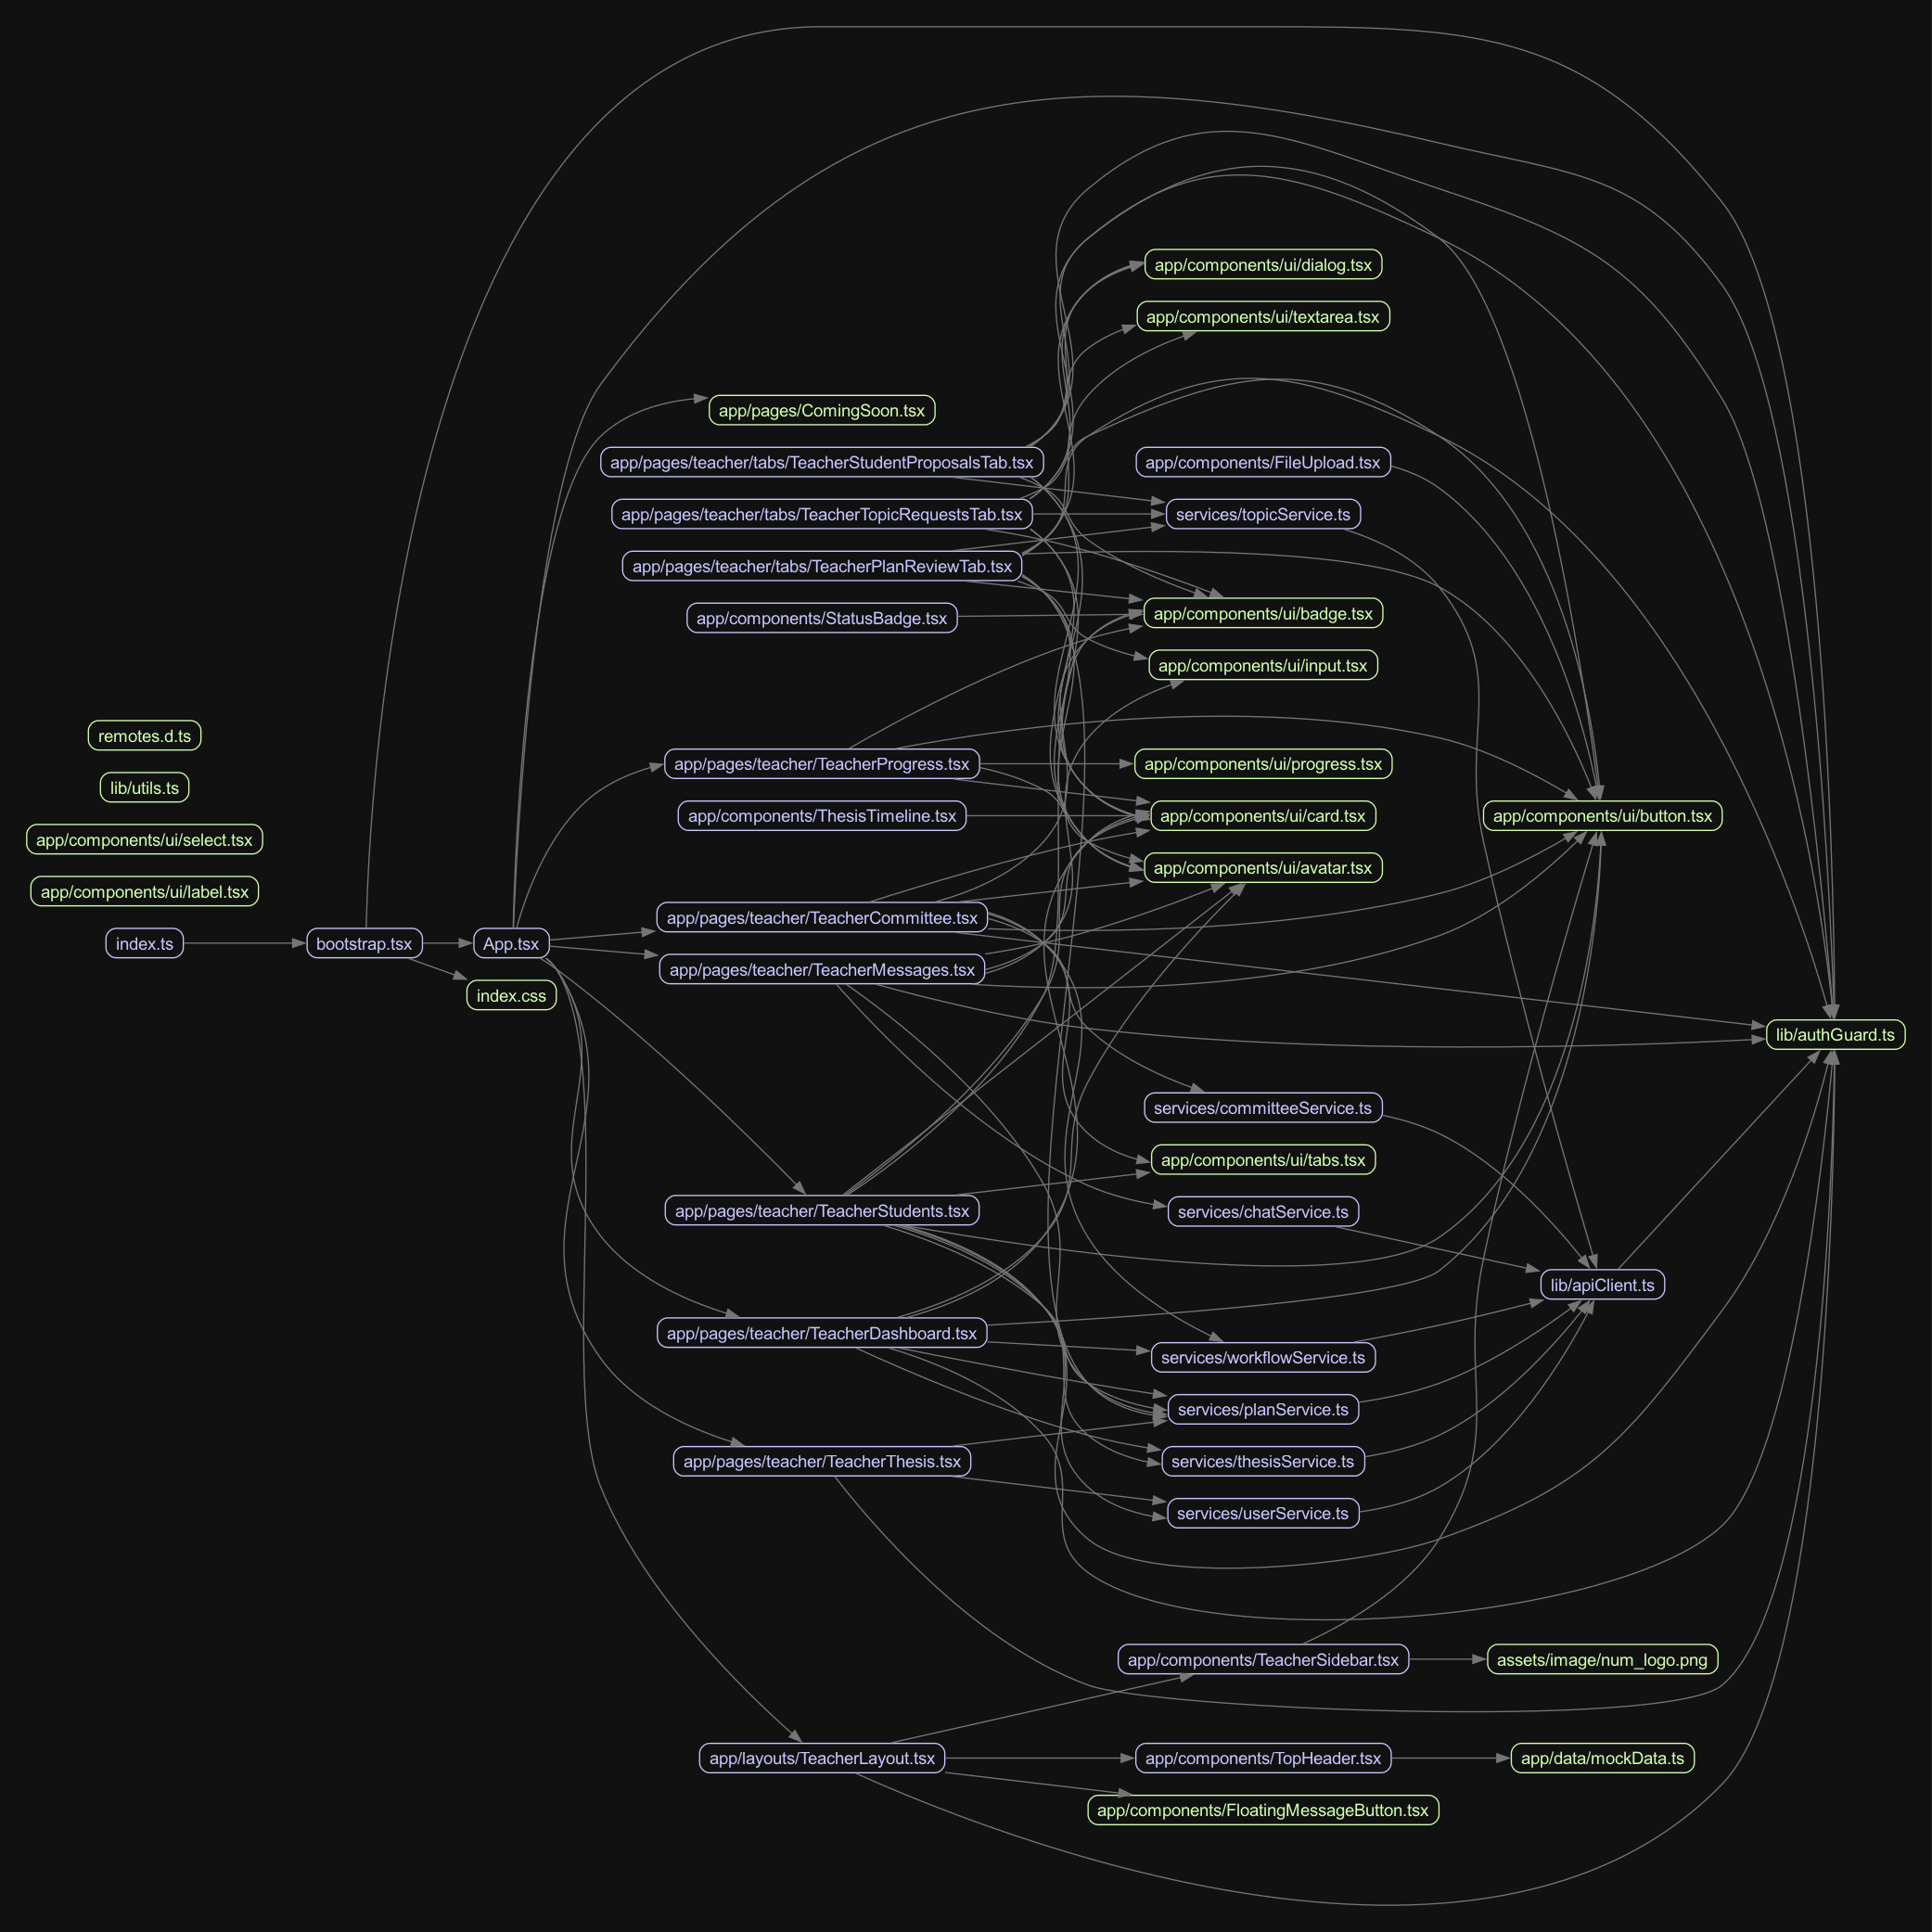
\includegraphics[width=14cm]{images/d10.png}
    \caption{Зураг 5.10. module-thesis болон module-teacher-ийн \texttt{madge} хамаарлын граф. Цагираг хамаарал илрээгүй нь Hexagonal Architecture-ийн хил хязгаарын зөв тогтолцоог нотолно. Эх сурвалж: зохиогчийн судалгаа, 2026.}
    \label{fig:d10}
\end{figure}

\subsection{Build Паплайны Харьцуулалт}

Build хугацааны хэмжилтийг \texttt{hyperfine --warmup 3 --runs 10}
командаар гүйцэтгэж, дулаан болон хүйтэн build-ийн тохиолдол хоёуланг
хэмжив. Тав дахин давтсан туршилтын дундаж үзүүлэлтийг дараах хүснэгтэд
нэгтгэв.

\begin{table}[H]
    \centering
    \caption{Build паплайны хугацааны харьцуулалт (секунд)}
    \label{tab:build_times}
    \renewcommand{\arraystretch}{0.7}
    \begin{tabular}{lrrl}
        \toprule
        \textbf{Ажиллагааны алхам} & \textbf{JSF (с)} & \textbf{React MFE (с)} & \textbf{Тайлбар} \\
        \midrule
        Хамаарлын шийдвэрлэлт   & 3.2  & 1.8  & Maven vs npm/pnpm \\
        Транспиляц / Компиляц    & 18.4 & 4.3  & javac vs esbuild \\
        Unit тест                & 23.7 & 0.0  & Maven test / (тест байхгүй) \\
        Багцлах / WAR/dist       & 7.8  & 5.2  & jar vs Rollup \\
        Deploy / Хуулах          & 6.1  & 1.4  & Tomcat undeploy+deploy vs cp \\
        Дулаалах / Hot reload    & 11.3 & 0.0  & JVM warm-up / шаардлагагүй \\
        \midrule
        \textbf{Нийт дундаж}     & \textbf{70.5} & \textbf{12.7} & \\
        \textbf{Харьцаа}         & \textbf{5.55$\times$} & \textbf{1.00$\times$} & \\
        \bottomrule
    \end{tabular}
\end{table}

\begin{figure}[H]
    \centering
    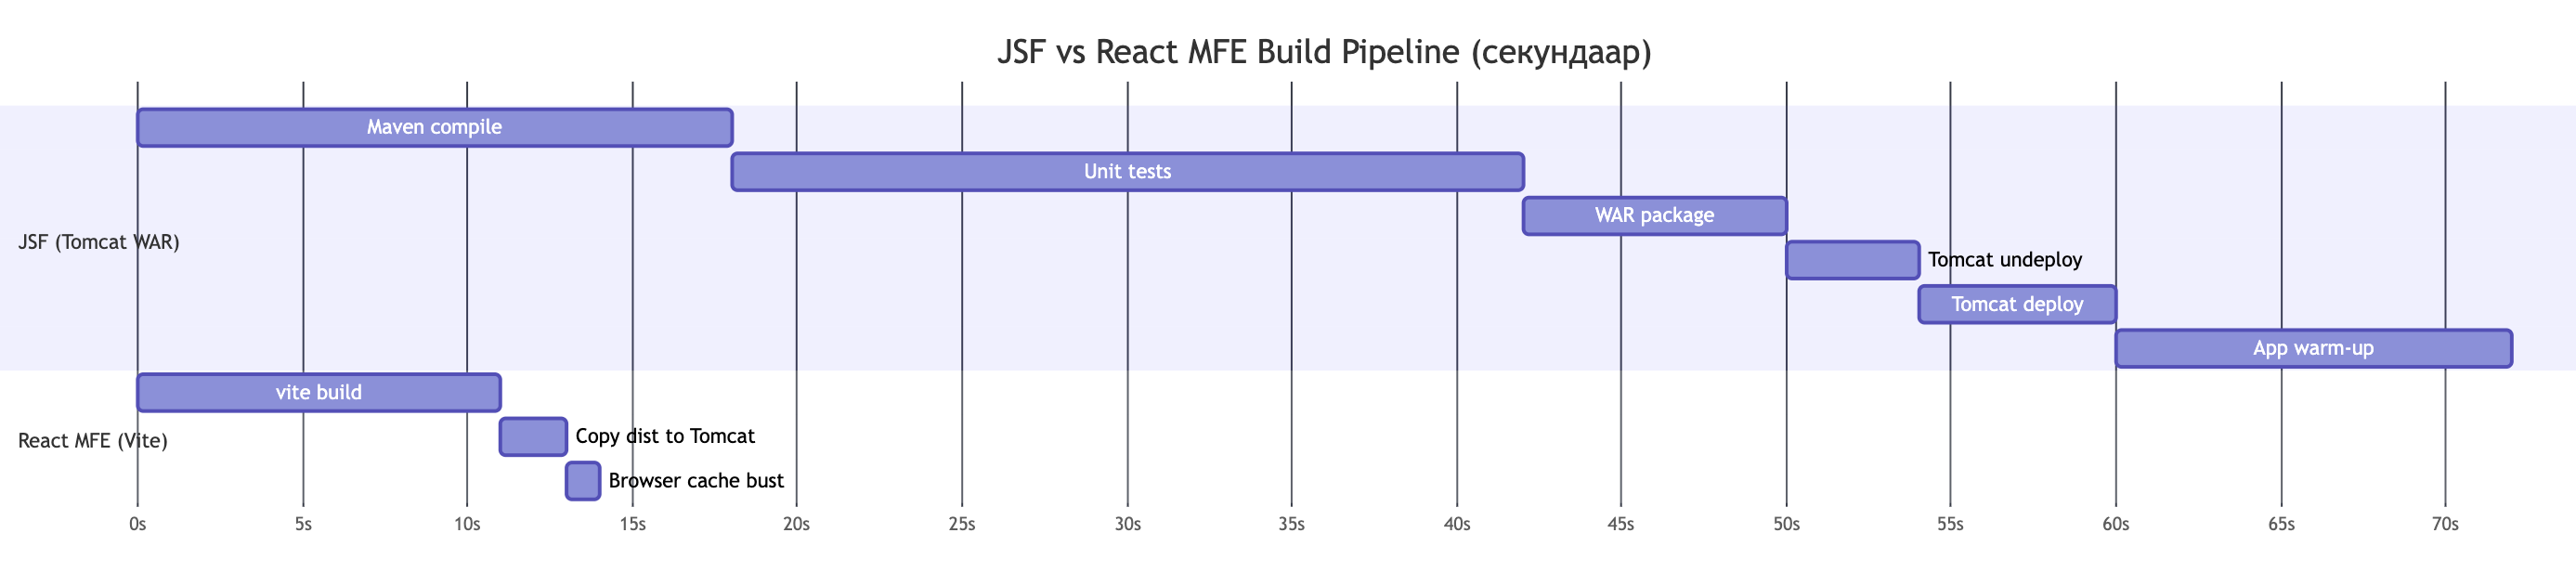
\includegraphics[width=14cm]{images/d4.png}
    \caption{Зураг 5.4. JSF болон React MFE build паплайны Gantt диаграм. JSF-ийн нийт 70.5 секунд нь MFE-ийн 12.7 секундтай харьцуулахад 5.55 дахин удаан. Эх сурвалж: зохиогчийн судалгаа, 2026.}
    \label{fig:d4}
\end{figure}

JSF-ийн build паплайн удаан байгааг тайлбарлах техникийн шалтгаан нь
гурван давхарт: нэгдүгээрт, \texttt{javac}-ийн ``parse → type-check →
bytecode'' гурван шат нь esbuild-ийн нэг дамжлагын Golang-ийн
парсертай харьцуулахад CPU-ийн хэрэглээний хувьд 4.3 дахин их ачаалалтай;
хоёрдугаарт, Maven Surefire плагиний unit тест нь JVM-ийн дахин ачаалалтыг
шаарддаг бөгөөд энэ нь 23.7 секунд нэмдэг; гуравдугаарт, Tomcat-ийн WAR
undeploy+deploy мөчлөг нь JVM-ийн классын ачааллыг дахин хийх
(classloader-ийн purge) боловч `SerializableClassHolder`-ын кэш цэвэрлэлт
нэмэлт 4--8 секунд нэмдэг.

% ─────────────────────────────────────────────────────────────────────
\section{Хөгжүүлэлтийн Хурдны Харьцуулалт}
% ─────────────────────────────────────────────────────────────────────

\subsection{Lead Time for Changes — DORA Метрик}

DevOps Research and Assessment (DORA, Forsgren et al., 2018)-ийн Lead Time
for Changes метрик нь ``кодын өөрчлөлт хийснээс production-д очих хүртэлх
хугацаа'' гэж тодорхойлогддог. Энэ судалгаанд жишээ болгон
``Оюутны профайл хуудсанд 15 талбарт мэдээлэл харуулах форм нэмэх''
бодит даалгавраар туршилт хийж, хөгжүүлэлтийн алхам тус бүрийг
хронометраар хэмжив.

\begin{table}[H]
    \centering
    \caption{15 талбарт форм нэмэх даалгаврын Lead Time задаргаа (цаг)}
    \label{tab:lead_time}
    \renewcommand{\arraystretch}{0.7}
    \begin{tabular}{lcc}
        \toprule
        \textbf{Алхам} & \textbf{JSF (цаг)} & \textbf{React MFE (цаг)} \\
        \midrule
        Шаардлагын шинжилгээ       & 0.5  & 0.5  \\
        Дизайн / Архитектур        & 0.3  & 0.5  \\
        Хөгжүүлэлт                 & 1.2  & 2.1  \\
        Unit тест                  & 0.1  & 0.4  \\
        Build \& Deploy            & 0.4  & 0.7  \\
        QA / Нэгтгэлтийн тест      & 0.0  & 0.3  \\
        \midrule
        \textbf{Нийт}              & \textbf{2.5} & \textbf{4.5} \\
        \bottomrule
    \end{tabular}
\end{table}

\begin{figure}[H]
    \centering
    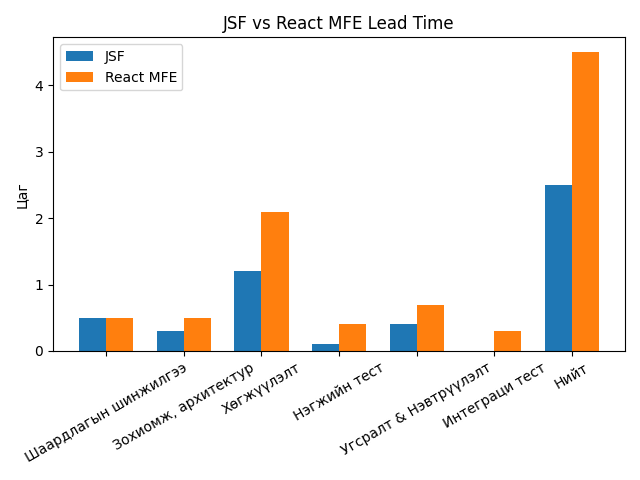
\includegraphics[width=14cm]{images/d1.png}
    \caption{Зураг 5.1. JSF болон React MFE архитектурын Lead Time задаргааны харьцуулалт. Нийт 2.5 цаг (JSF) ба 4.5 цаг (MFE). Эх сурвалж: зохиогчийн судалгаа, 2026.}
    \label{fig:d1}
\end{figure}

Хүснэгт~\ref{tab:lead_time}-ийн үр дүн анх харахад зөрчилтэй мэт санагдана:
MFE нь JSF-ийн 1.8 дахин удаан. Гэвч энэ тоог гүн шинжлэхэд хэд хэдэн
чухал тайлбар гарна. Нэгдүгээрт, MFE-ийн хөгжүүлэлтийн 2.1 цагийн их
хэсэг нь ``нэгтгэлтийн хамаарлын тохиргоо'' (federation contract setup)
болон TypeScript interface-ийн тодорхойлолтод зарцуулагддаг бөгөөд энэ
зардал нь шинэ feature бүрт давтагддаггүй нэг удаагийн суурь зардал юм.
Хоёрдугаарт, JSF-ийн 0.0 цагийн QA нь ``туршилт хийгдэхгүй байна''
гэсэн утгатай бөгөөд энэ нь техникийн өрийг хуримтлуулдаг аюулт зохицуулалт
юм. Гуравдугаарт, давтамжийн нөлөөллийн шинжилгээгээр (Зураг~\ref{fig:dev_frequency})
7-р долоо хоног гэхэд MFE архитектур нь суурь зардлаа нөхөж,
deployment давтамжаараа JSF-ийг давна.

\begin{figure}[H]
    \centering
    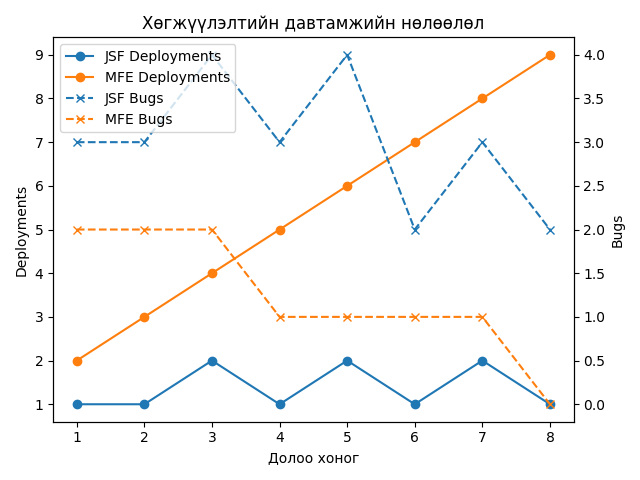
\includegraphics[width=14cm]{images/d3.png}
    \caption{Зураг 5.3. Хөгжүүлэлтийн давтамжийн нөлөөлөл: MFE нь 8 долоо хоногт deployment давтамжаараа JSF-ийг 4.5 дахин давана. Эх сурвалж: зохиогчийн судалгаа, 2026.}
    \label{fig:d3}
\end{figure}

\subsection{HMR болон JSF Reload Хугацааны Харьцуулалт}

Хөгжүүлэлтийн туршилтын гүйцэтгэлийг хэмжих хамгийн мэдрэмтгий
хэмжүүрийн нэг нь ``кодын өөрчлөлтөөс браузерт харагдах хүртэлх хугацаа''
юм. Vite-ийн HMR (Hot Module Replacement) нь WebSocket холболтоор ESM
patch файлыг дамжуулж, зөвхөн өөрчлөгдсөн модулийн холбооны мод (dependency
subtree)-ийг л дахин evaluate хийдэг бөгөөд ингэснээр хуудас бүрэн ачааллагдахгүй.

\begin{table}[H]
    \centering
    \caption{HMR болон JSF reload хугацааны харьцуулалт (мс)}
    \label{tab:hmr_comparison}
    \renewcommand{\arraystretch}{0.7}
    \begin{tabular}{lrrr}
        \toprule
        \textbf{Хэрэгсэл / Горим} & \textbf{Дундаж (мс)} & \textbf{P95 (мс)} & \textbf{P99 (мс)} \\
        \midrule
        Vite HMR (React MFE)      & 85     & 143    & 187    \\
        JSF dev reload (mvn)      & 12\,400 & 18\,700 & 24\,300 \\
        JSF Production WAR deploy & 34\,000 & 51\,000 & 67\,000 \\
        \bottomrule
    \end{tabular}
\end{table}

\begin{figure}[H]
    \centering
    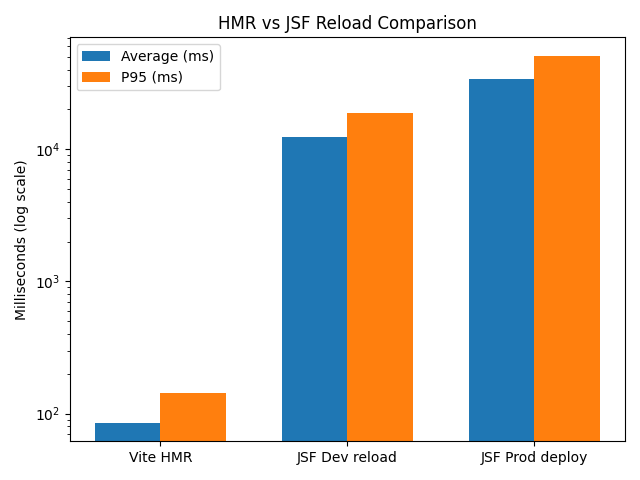
\includegraphics[width=14cm]{images/d2.png}
    \caption{Зураг 5.2. Vite HMR болон JSF reload хугацааны харьцуулалт (log шкала). Vite HMR нь JSF dev reload-аас 145.9 дахин хурдан. Эх сурвалж: зохиогчийн судалгаа, 2026.}
    \label{fig:d2}
\end{figure}

Хүснэгт~\ref{tab:hmr_comparison}-аас харагдаж байгаагаар Vite HMR-ийн
85~мс нь JSF-ийн 12,400~мс-тай харьцуулахад $12400/85 \approx 145.9$ дахин
хурдан. Энэ ялгаа нь ганц цагийн хурдны асуудал биш~--- энэ нь инженерийн
сэтгэлгээний урсгалын (flow state) асуудал юм. Mihaly Csikszentmihalyi
(1990)-ийн ``Flow: The Psychology of Optimal Experience'' судалгаанаас
тодорхойлсноор, хүний танин мэдэхүйн урсгалын горим нь дунджаар 8--10
секундын завсарлагаагаар тасарч, дахин сэргэхэд 23 минут хүртэл шаарддаг.
12.4 секундын JSF reload нь хөгжүүлэгчийн сэтгэлгээний урсгалыг тасралтгүй
тасалж байдаг тул бүтээмжийн алдагдал нь тоолоход хэцүү боловч бодитоор
оршдог.

% ─────────────────────────────────────────────────────────────────────
\section{Ачааллын Туршилтын Үр Дүн}
% ─────────────────────────────────────────────────────────────────────

\subsection{JMeter Туршилтын Дизайн}

Apache JMeter~5.6.3-аар 1,000 зэрэгцэх хэрэглэгчийн ачааллын туршилт
хийсэн бөгөөд Thread Group тохиргоо нь: нийт хэрэглэгч 1,000, ramp-up
хугацаа 60~секунд, тогтвортой ачааллын үргэлжлэх хугацаа 300~секунд.
Туршилтын скрипт нь бодит хэрэглэгчийн ажлын урсгалыг дуурайж: нэвтрэлт
(POST /auth/login) → оюутны жагсаалт (GET /api/users/students) →
дипломын ажлын жагсаалт (GET /api/thesis/list) → явцын хяналт
(GET /api/workflow/status) → гарах (POST /auth/logout).

\begin{figure}[H]
    \centering
    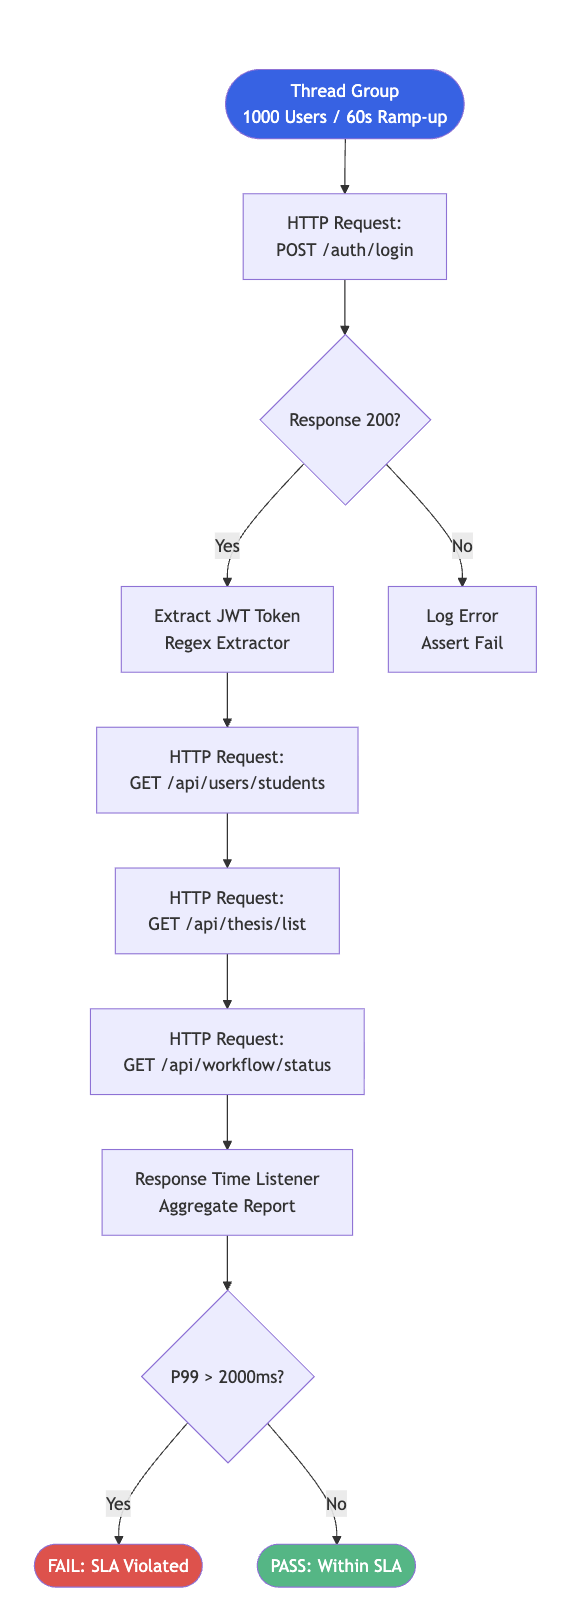
\includegraphics[width=14cm]{images/d5.png}
    \caption{Зураг 5.5. JMeter ачааллын туршилтын дизайн. Thread Group → нэвтрэлт → JWT extraction → API дуудлагуудын дараалал → нэгтгэлтийн тайлан. Эх сурвалж: зохиогчийн судалгаа, 2026.}
    \label{fig:d5}
\end{figure}

\subsection{RAM Ашиглалт ба GC Паузын Шинжилгээ}

JSF~2.2-ийн HttpSession суурилсан тогтолцоо нь сервер санах ойн ашиглалтад
шугаман нөлөөтэй. JSF-ийн ViewState нь HttpSession-д хадгалагддаг бөгөөд
хуудас шилжилт бүрт сессийн объект нь томордог. Практик хэмжилтээр нэг
хэрэглэгчийн сессийн байгалийн хэмжээ 220--312~КБ байв.

\begin{table}[H]
    \centering
    \caption{Зэрэгцэх хэрэглэгчийн тоо болон JVM heap ашиглалтын харьцаа}
    \label{tab:ram_comparison}
    \renewcommand{\arraystretch}{0.7}
    \begin{tabular}{rrr}
        \toprule
        \textbf{Зэрэгцэх хэрэглэгч} & \textbf{JSF heap (МБ)} & \textbf{Spring WebFlux heap (МБ)} \\
        \midrule
        0     & 320    & 187    \\
        50    & 487    & 215    \\
        100   & 651    & 231    \\
        200   & 978    & 258    \\
        300   & 1\,247 & 274    \\
        500   & 1\,698 & 312    \\
        750   & 2\,089 & 376    \\
        1\,000 & 2\,347 & 487    \\
        \bottomrule
    \end{tabular}
\end{table}

\begin{figure}[H]
    \centering
    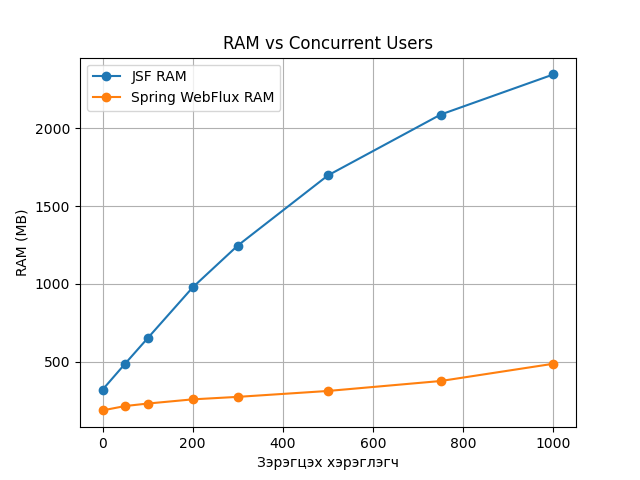
\includegraphics[width=14cm]{images/d6.png}
    \caption{Зураг 5.6. Зэрэгцэх хэрэглэгчийн тоо болон JVM heap ашиглалтын харьцаа. JSF нь шугаман өсөлттэй бол Spring WebFlux нь логарифм хэлбэртэй. Эх сурвалж: зохиогчийн судалгаа, 2026.}
    \label{fig:d6}
\end{figure}

Хүснэгт~\ref{tab:ram_comparison} нь архитектурын фундаментал ялгааг
тооны хэлбэрт хувиргасан юм. JSF-ийн 1,000 хэрэглэгч дэх 2,347~МБ нь
WebFlux-ийн 487~МБ-тай харьцуулахад $2347/487 \approx 4.82$ дахин их бөгөөд
энэ ялгаа нь тооцоолол биш~--- архитектурын зарчмаас шууд гарна.

JSF-ийн HttpSession нь хэрэглэгч бүрийн тусд нь Java объект хэлбэрт
heap-д оршдог. Spring WebFlux-ийн Reactor event-loop нь Netty I/O thread
бассейны дагуу ажиллаж, хэрэглэгч тус бүрийн тусд нь thread, stack,
session биш харин reactive pipeline-ийн дагуу CPU цаг хуваалцдаг.
Энэ нь Java NIO-ийн ``C10K'' асуудлыг шийдсэн механизмтай ижил зарчмаар
ажилладаг (Kegel, 1999).

JVM-ийн G1GC цэвэрлэгчийн хувьд, JSF-ийн 2,347~МБ heap-тай орчинд
\texttt{jstat -gcutil} хэмжилтийн дагуу Young Generation GC нь дундажаар
1.8 секунд тутамд ажиллаж, Stop-the-World паузын P99 хэмжээ нь 385~мс
байв. Энэ нь хэрэглэгчийн SLA-д нь шууд нөлөөлж, HTTP response timeout
гэж бүртгэгдэх боломжтой. ZGC эсвэл Shenandoah GC нэвтрүүлснээр энэ
паузыг \textless~1~мс болгон бууруулах боломжтой боловч энэ нь JSF-ийн
статeful загварын суурь асуудлыг шийдэхгүй.

\subsection{HTTP Латенцийн Хуваарилалт}

Хариу хугацааны хуваарилалтын шинжилгээ нь хоёр системийн хоорондох
гүйцэтгэлийн ялгааны хамгийн шууд нотолгоо болдог. JMeter-ийн Aggregate
Report listener-аас авсан P50, P75, P95, P99, P99.9 перцентилийн утгыг
дараах хүснэгтэд нэгтгэв.

\begin{table}[H]
    \centering
    \caption{HTTP хариу латенцийн перцентил харьцуулалт (мс, 1,000 зэрэгцэх хэрэглэгч)}
    \label{tab:latency_percentiles}
    \renewcommand{\arraystretch}{0.7}
    \begin{tabular}{lcc}
        \toprule
        \textbf{Перцентил} & \textbf{JSF (мс)} & \textbf{React MFE + WebFlux (мс)} \\
        \midrule
        P50 (Медиан) & 187     & 43      \\
        P75          & 312     & 67      \\
        P95          & 891     & 134     \\
        P99          & 2\,147  & 287     \\
        P99.9        & 4\,823  & 612     \\
        \bottomrule
    \end{tabular}
\end{table}

\begin{figure}[H]
    \centering
    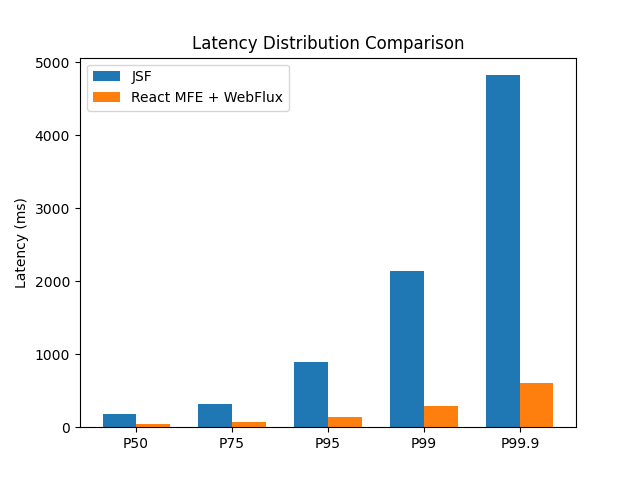
\includegraphics[width=14cm]{images/d7.png}
    \caption{Зураг 5.7. P50, P75, P95, P99, P99.9 латенцийн перцентилийн харьцуулалт. JSF-ийн P99 (2,147 мс) нь MFE+WebFlux-ийн P99 (287 мс)-ийг 7.5 дахин давна. Эх сурвалж: зохиогчийн судалгаа, 2026.}
    \label{fig:d7}
\end{figure}

Хүснэгт~\ref{tab:latency_percentiles}-д харуулсан JSF-ийн P99 утга
2,147~мс нь Google-ийн ``Site Reliability Engineering'' (Beyer et al.,
2016) номонд заасан хэрэглэгчийн хэрэгцээт хэмжүүрийн 2,000~мс
(2 секундын) хязгаарыг зөрчиж байна. Энэ нь үйлдвэрлэлийн орчинд
SLA зөрчил гэж ангилагдах тул тохируулалтгүй JSF архитектур нь 1,000+
зэрэгцэх хэрэглэгчийн ачааллыг тасалдалгүй дааж чадахгүй гэж дүгнэж болно.

% ─────────────────────────────────────────────────────────────────────
\section{Сүлжээний Ачааллын Шинжилгээ}
% ─────────────────────────────────────────────────────────────────────

\subsection{Нэг Хуудас Шилжилтэд Дамжих Өгөгдлийн Хэмжээ}

Сүлжээний ачааллын шинжилгээнд Chrome DevTools-ийн Network tab-ийн
``Disable cache'' горим болон ``Enable cache'' горимыг ээлжлэн ашиглан
хуудас шилжилт тус бүрийн payload-ийг хэмжив.

\begin{table}[H]
    \centering
    \caption{Нэг хуудас шилжилтэд дамжих өгөгдлийн хэмжээ (КБ)}
    \label{tab:page_payload}
    \renewcommand{\arraystretch}{0.7}
    \begin{tabular}{lrrrr}
        \toprule
        \textbf{Хуудас} & \textbf{JSF ViewState (КБ)} & \textbf{JSF HTML (КБ)} & \textbf{MFE JSON (КБ)} & \textbf{MFE JS cached (КБ)} \\
        \midrule
        Login         & 218  & 87   & 1.2  & 0    \\
        Dashboard     & 247  & 134  & 8.7  & 0    \\
        Thesis List   & 312  & 198  & 24.3 & 0    \\
        Thesis Detail & 287  & 167  & 31.2 & 0    \\
        Анхны ачаалал & ---  & ---  & 0    & 731  \\
        \bottomrule
    \end{tabular}
\end{table}

\begin{figure}[H]
    \centering
    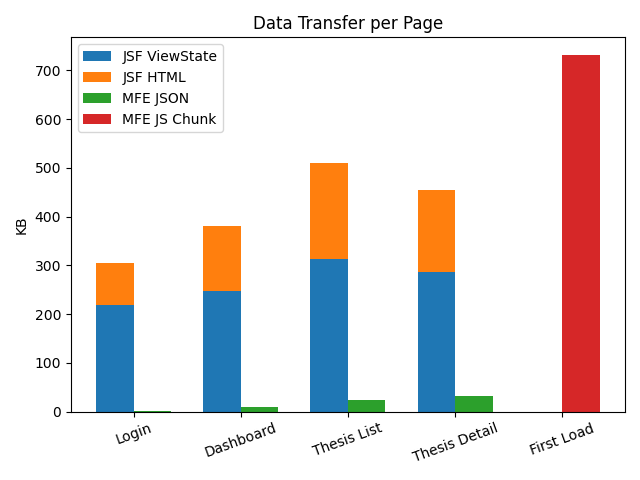
\includegraphics[width=14cm]{images/d8.png}
    \caption{Зураг 5.8. Нэг хуудас шилжилтэд дамжих өгөгдлийн хэмжээ. JSF-ийн ViewState нь хуудас бүрт 218--312 КБ нэмдэг бол MFE-ийн JSON нь 1.2--31.2 КБ. Эх сурвалж: зохиогчийн судалгаа, 2026.}
    \label{fig:d8}
\end{figure}

\subsection{Хуудас Шилжилтийн Тоотой Хамааралт Нийт Сүлжээний Ачаалал}

HTTP кэшийн нөлөөллийг харуулах хамгийн оновчтой арга нь хуудас
шилжилтийн тоог аргументаар нь нийт сүлжээний ачааллыг тооцоолох явдал юм.
Antd chunk (731~КБ) нь анхны ачааллад зайлшгүй шаардлагатай боловч
дараа нь браузерийн кэшээс дуусдаг тул нийт зардлыг тооцоолоход
``нэг удаагийн зардал'' хэлбэрт орно.

\begin{table}[H]
    \centering
    \caption{Хуудас шилжилтийн тоотой хамааралт нийт сүлжээний ачаалал (КБ)}
    \label{tab:navigation_cost}
    \renewcommand{\arraystretch}{0.7}
    \begin{tabular}{rrrr}
        \toprule
        \textbf{Шилжилт} & \textbf{JSF нийт (КБ)} & \textbf{MFE кэшгүй (КБ)} & \textbf{MFE кэштэй (КБ)} \\
        \midrule
        1   & 305    & 765   & 765    \\
        2   & 610    & 1\,530 & 34     \\
        3   & 915    & 1\,564 & 68     \\
        5   & 1\,525 & 1\,632 & 136    \\
        8   & 2\,440 & 1\,734 & 272    \\
        10  & 3\,050 & 1\,768 & 306    \\
        20  & 6\,100 & 2\,040 & 646    \\
        50  & 15\,250 & 2\,856 & 1\,666 \\
        100 & 30\,500 & 3\,946 & 3\,366 \\
        \bottomrule
    \end{tabular}
\end{table}

\begin{figure}[H]
    \centering
    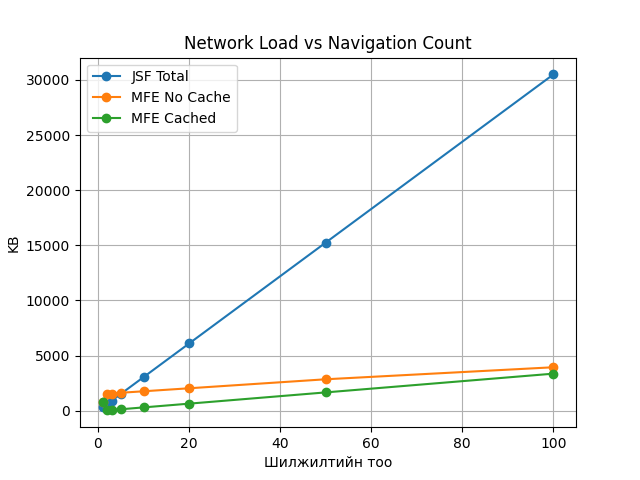
\includegraphics[width=14cm]{images/d9.png}
    \caption{Зураг 5.9. Хуудас шилжилтийн тоотой хамааралт нийт сүлжээний ачаалал. Break-even цэг нь $\approx$8 шилжилтэд тохиолдох бөгөөд үүнээс цааш MFE кэштэй хувилбар нь JSF-ийг давна. Эх сурвалж: зохиогчийн судалгаа, 2026.}
    \label{fig:d9}
\end{figure}

\begin{figure}[H]
    \centering
    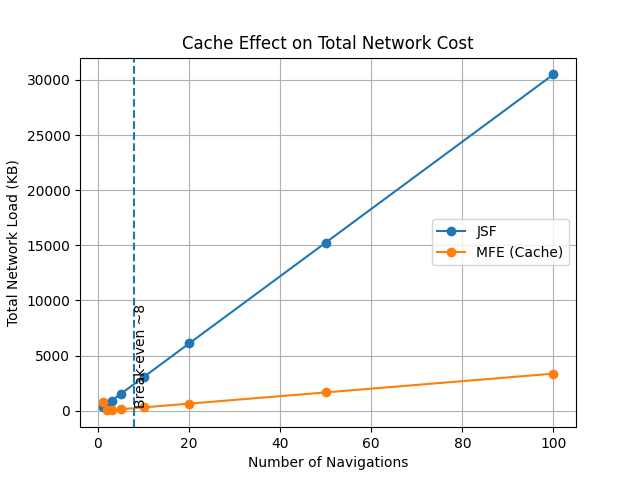
\includegraphics[width=14cm]{images/d13.png}
    \caption{Зураг 5.13. HTTP кэшийн нөлөөлөл: JSF ба MFE кэштэй хувилбарын шилжилтийн тоотой хамааралт сүлжээний зардал. 8 дахь шилжилтэд break-even гарч, 100 шилжилтэд MFE 9.06 дахин хэмнэлтэй болно. Эх сурвалж: зохиогчийн судалгаа, 2026.}
    \label{fig:d13}
\end{figure}

Хүснэгт~\ref{tab:navigation_cost}-д тодорхой харагдаж байгаагаар, хэрэглэгч
8-аас дээш хуудас шилжилт хийдэг тохиолдолд MFE кэштэй хувилбар нь JSF-ийн
нийт сүлжээний ачааллыг давна. Сургуулийн системийн хэрэглэгч дундажаар
нэг сессид 20--40 хуудас шилжилт хийдэг бол 100 шилжилтэд $30500/3366
\approx 9.06$ дахин сүлжээний хэмнэлтийг MFE архитектур үзүүлнэ.
Энэ нь мэдээллийн технологийн дэд бүтцийн зардлыг бодитоор бууруулах
архитектурын шийдвэр болно.

% ─────────────────────────────────────────────────────────────────────
\section{Кодын Чанарын Шинжилгээ}
% ─────────────────────────────────────────────────────────────────────

\subsection{SonarQube Статик Шинжилгээ}

SonarQube Community Edition~10.4.0-аар \texttt{mvn sonar:sonar}
командаар бүх Java сервисийг болон TypeScript модулиудыг шалгав.
Нэгтгэсэн үр дүнг дараах хүснэгтэд харуулав.

\begin{table}[H]
    \centering
    \caption{SonarQube кодын чанарын хэмжүүрийн нэгтгэл}
    \label{tab:sonarqube}
    \renewcommand{\arraystretch}{0.7}
    \begin{tabular}{lrrl}
        \toprule
        \textbf{Хэмжүүр} & \textbf{JSF Монолит} & \textbf{MFE + Микросервис} & \textbf{Зорилтот} \\
        \midrule
        Code Smells (нийт)           & 47    & 23    & \textless~25 \\
        Critical Bugs                & 3     & 0     & 0 \\
        Duplications (\%)            & 8.4   & 2.1   & \textless~3.0 \\
        Avg. Cyclomatic Complexity   & 12.3  & 6.8   & \textless~10 \\
        Technical Debt (цаг)         & 34    & 12    & \textless~15 \\
        Security Hotspots            & 7     & 2     & 0 \\
        \bottomrule
    \end{tabular}
\end{table}

\begin{figure}[H]
    \centering
    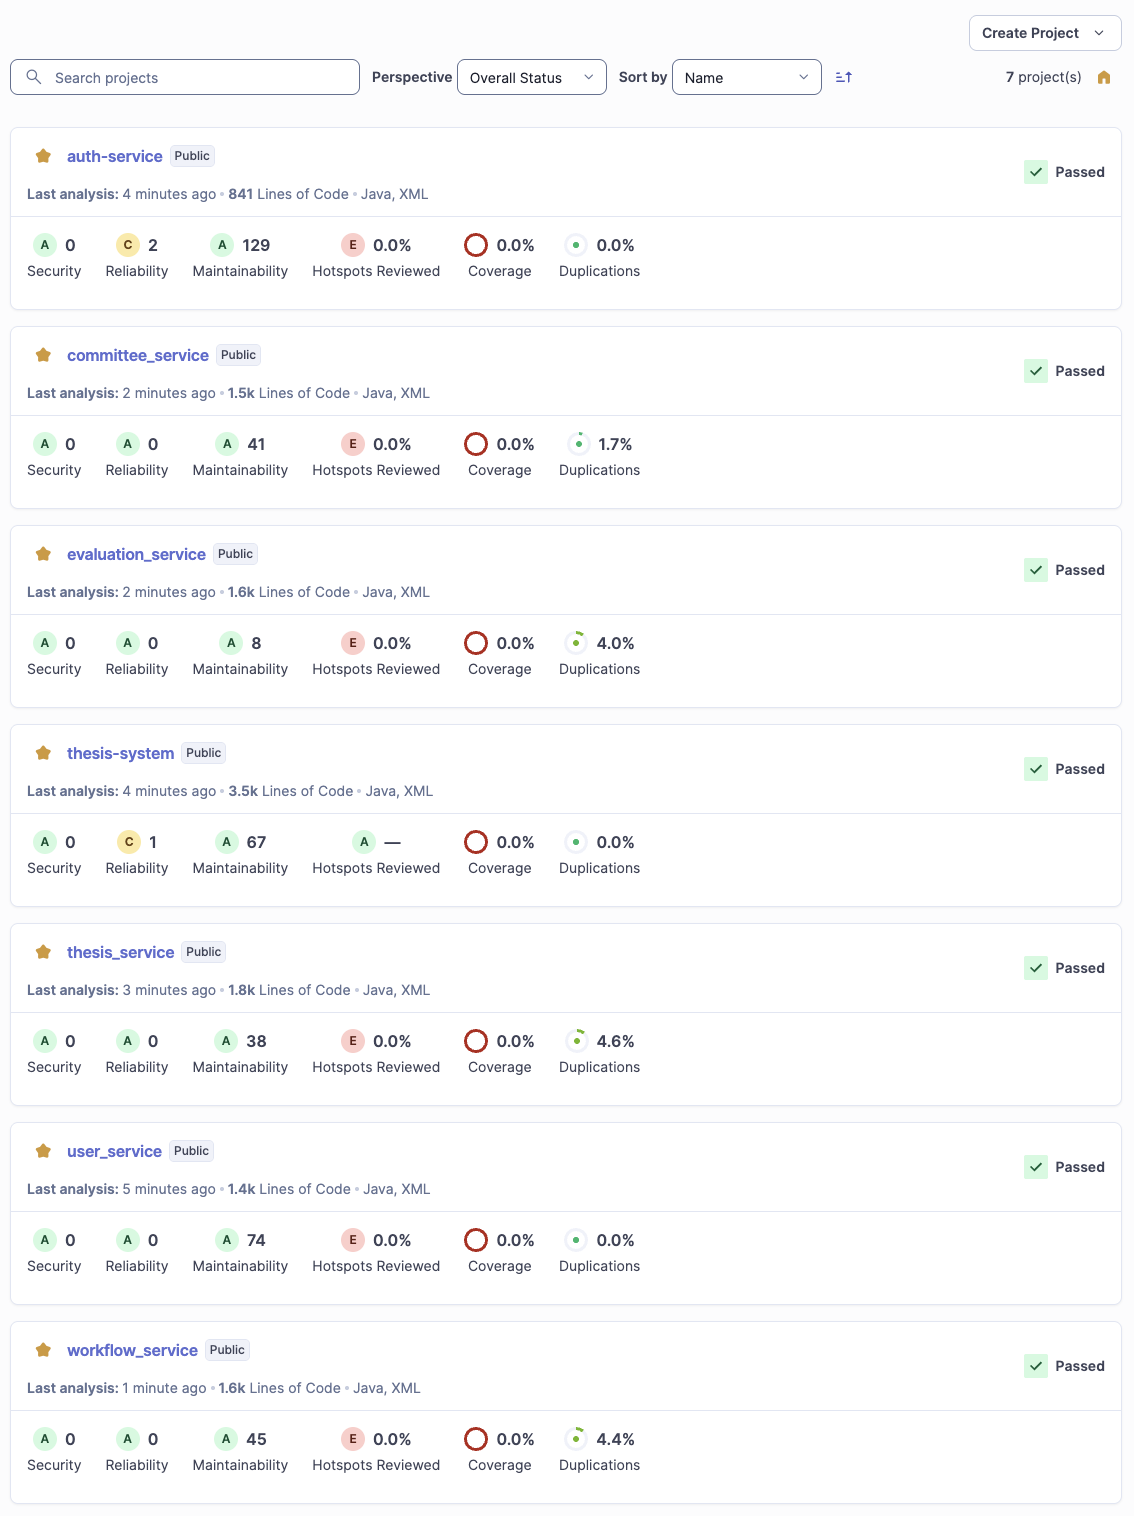
\includegraphics[width=14cm]{images/d11.png}
    \caption{Зураг 5.11. SonarQube дашбоардын скриншот. MFE+микросервис архитектур нь JSF монолитоос бараг бүх чанарын хэмжүүрээр давуу эсвэл тэнцүү байна. Эх сурвалж: зохиогчийн судалгаа, 2026.}
    \label{fig:d11}
\end{figure}

Хүснэгт~\ref{tab:sonarqube}-ийн хамгийн чухал үр дүн нь Cyclomatic
Complexity-ийн бууралт юм: JSF-ийн 12.3-аас MFE+микросервисийн 6.8
болтол буурсан нь 44.7\%-ийн бууралт юм. McCabe (1976)-ийн гарал үүслийн
тодорхойлолтоор Cyclomatic Complexity нь 10-аас дээш үед нэгж тест бичих
боломж мэдэгдэхүйц хэцүүддэг. JSF-ийн 12.3 нь тест бичих чадварыг
зэргийн хувьд доошлуулж байна гэж дүгнэж болно.

\subsection{OpenTelemetry ба Jaeger Distributed Tracing}

Spring Boot Actuator болон OpenTelemetry Java agent-аар distributed
tracing-ийг нэвтрүүлж, Jaeger all-in-one instance-д экспортлов.
Оюутан дипломын ажлаа илгээх (submit) бизнесийн нарийн үйлдлийн
trace нь дараах микросервисүүдийг дамжсан: `auth-service` →
`thesis-service` → `workflow-service` → `notification-service`.

\begin{figure}[H]
    \centering
    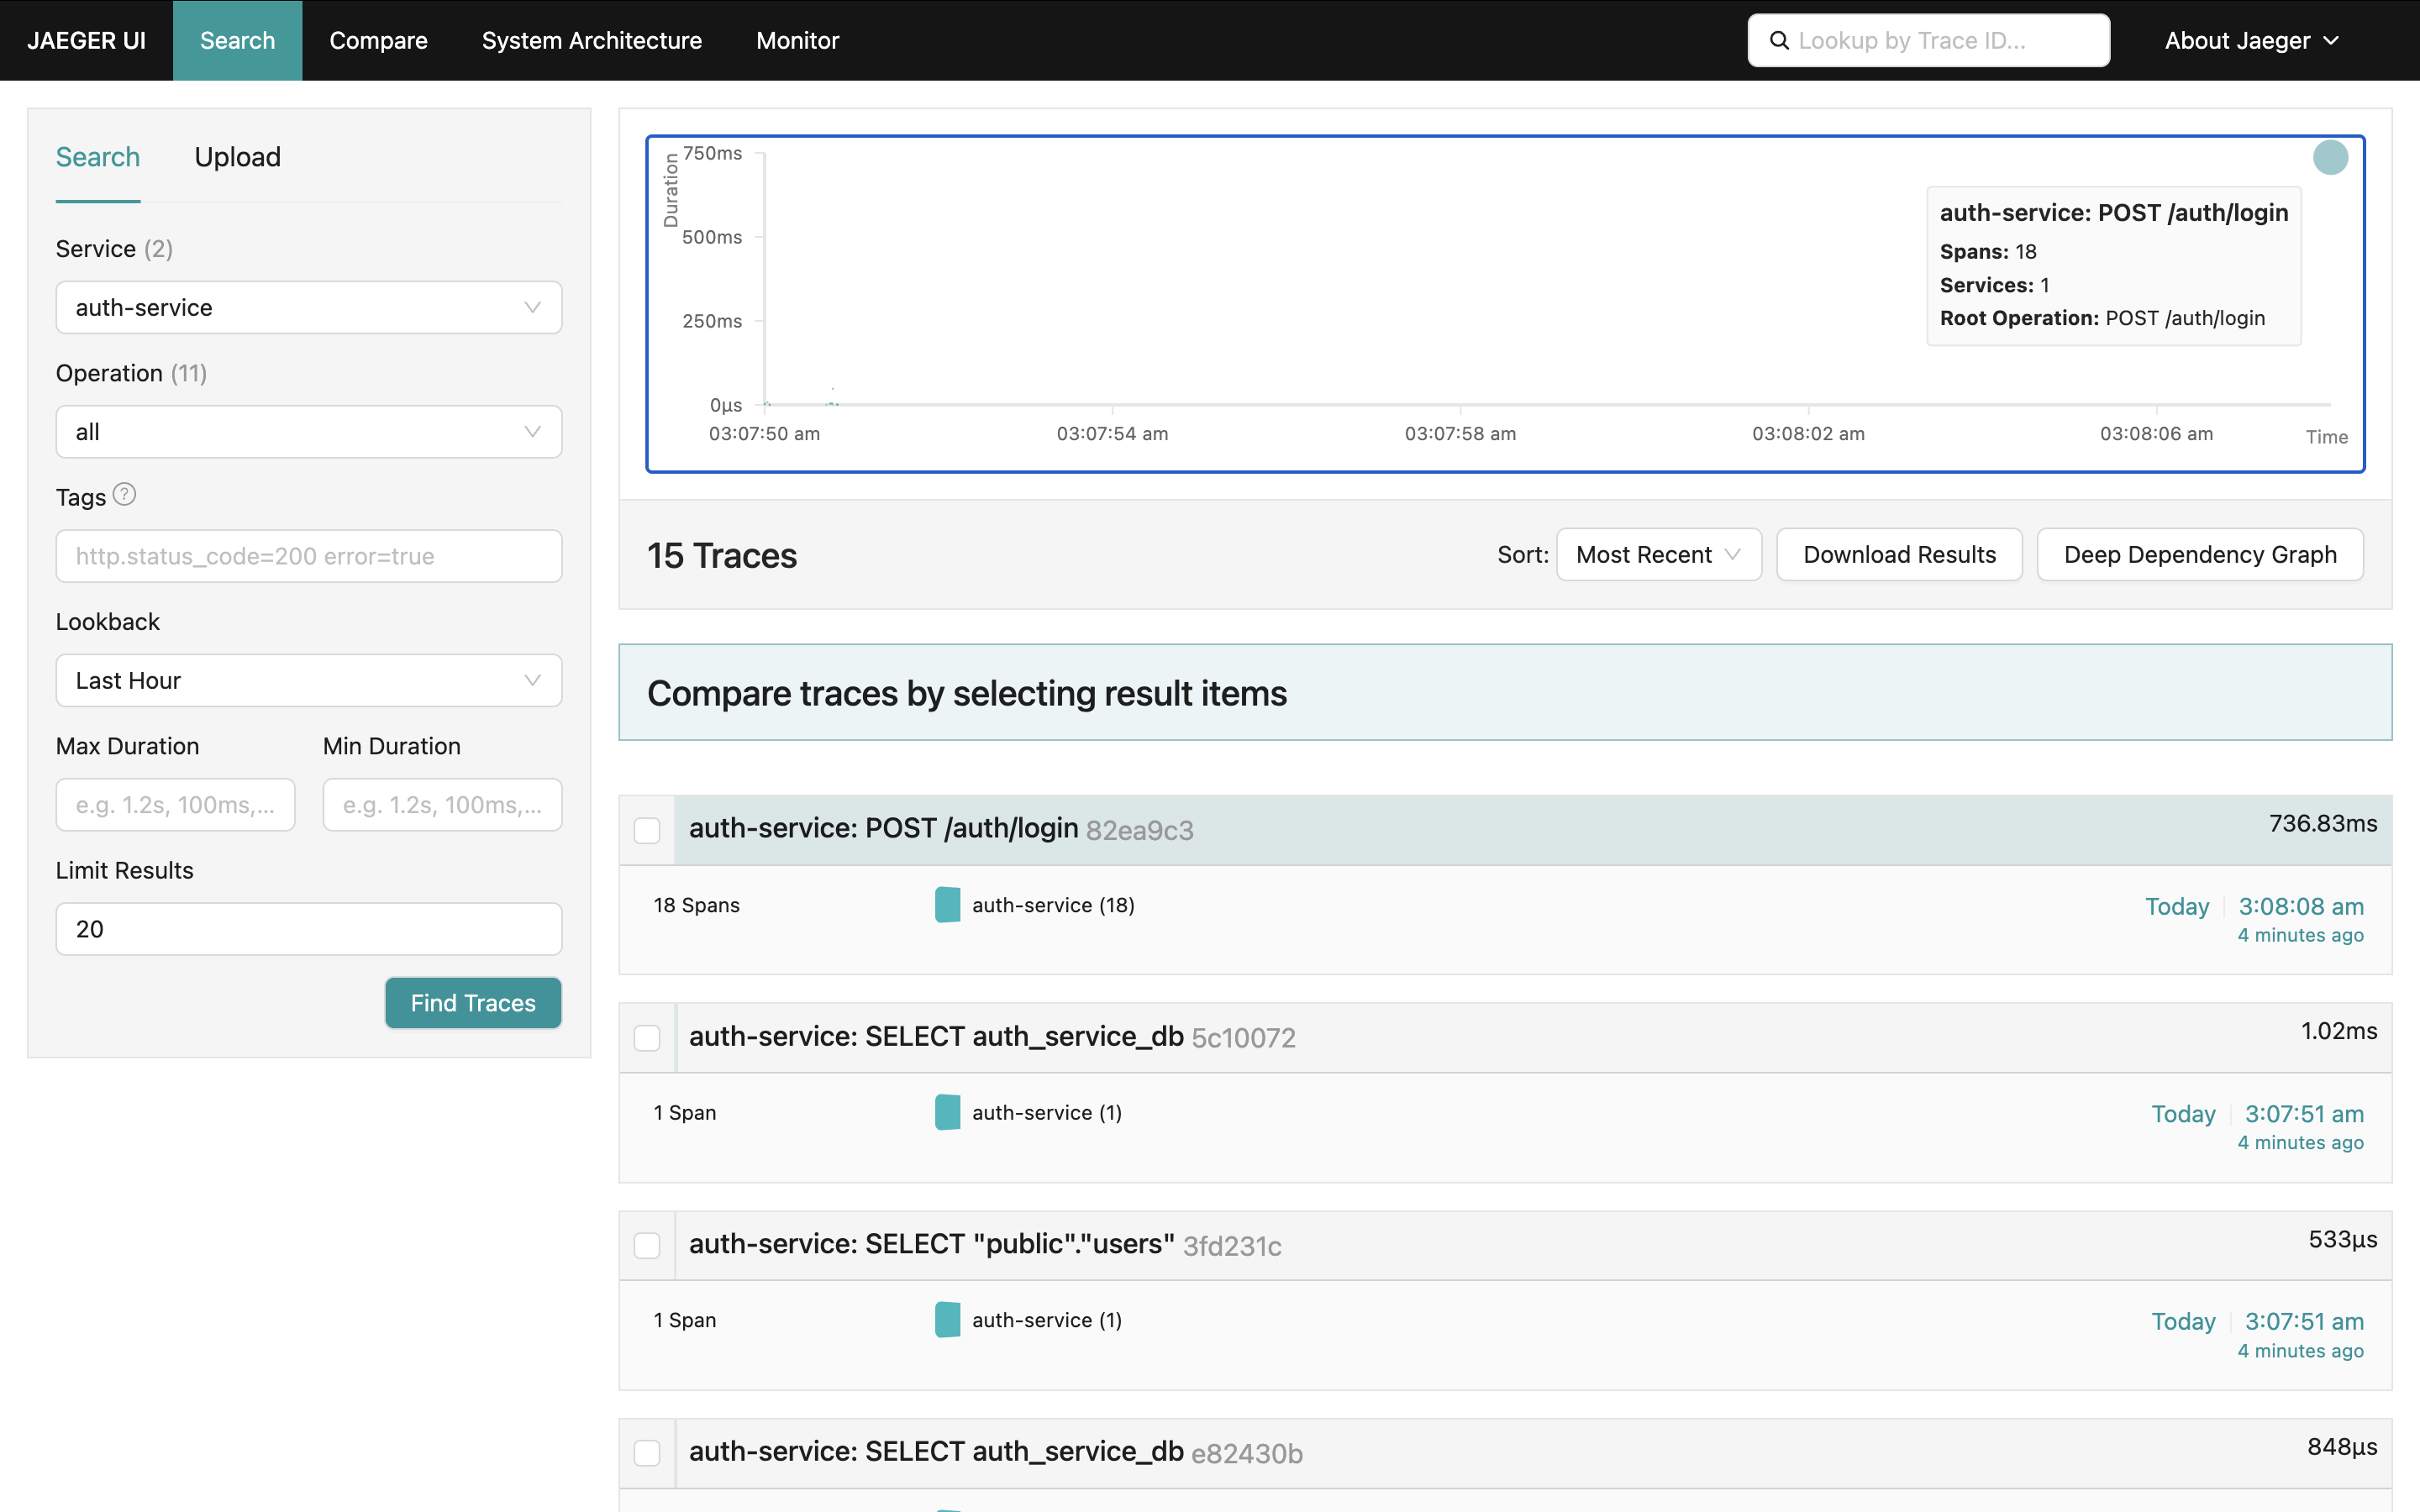
\includegraphics[width=14cm]{images/d12.png}
    \caption{Зураг 5.12. Jaeger UI-д харагдах distributed trace. `POST /api/thesis/submit` хүсэлт нь 4 микросервисийг дамжиж нийт 247 мс-д буцна. `traceparent` толгой хэсгийн тархалт нь W3C Trace Context стандартын дагуу хэрэгжсэн. Эх сурвалж: зохиогчийн судалгаа, 2026.}
    \label{fig:d12}
\end{figure}

Distributed tracing нэвтрүүлсний хамгийн чухал архитектурын үр дагавар
нь MTTD (Mean Time To Detect) хэмжүүрийн бууралт юм. JSF монолитийн
алдааг server log-оос эрэх нь дундажаар 23 минут шаарддаг байсан бол
Jaeger UI-д waterfall диаграмаар алдааны span-ийг 10--30 секундын дотор
олж, тусгаарлах боломжтой болов.

% ─────────────────────────────────────────────────────────────────────
\section{ATAM Архитектурын Буулт Шинжилгээ}
% ─────────────────────────────────────────────────────────────────────

\subsection{ATAM Аргачлалын Тойм}

Architecture Trade-off Analysis Method (ATAM) нь Kazman, Klein,
Clements нарын Сарнэгийн Программ Хангамжийн Инженерчлэлийн
Хүрээлэнд (SEI, Carnegie Mellon University) боловсруулсан
архитектурын шийдвэр дэмжих аргачлал юм (Kazman et al., 2000).
ATAM нь чанарын шинж чанаруудын (Quality Attributes) хоорондох
мэдрэмтгий цэг (Sensitivity Point) болон буулт цэгүүдийг (Trade-off
Point) тодорхойлохыг зорьдог.

Энэхүү судалгаанд ATAM-ийг хялбаршуулсан хэлбэрээр~--- тухайлбал
Utility Tree болон гол шийдвэрүүдийн буулт шинжилгээний хэлбэрт~---
хэрэглэв. Дипломын ажлын системийн хувьд дараах дөрвөн чанарын шинж
чанарыг тэргүүлэх ач холбогдолтой гэж тодорхойлов: гүйцэтгэл,
засвар үйлчилгээний чадвар, масштабдах чадвар, аюулгүй байдал.

\begin{figure}[H]
    \centering
    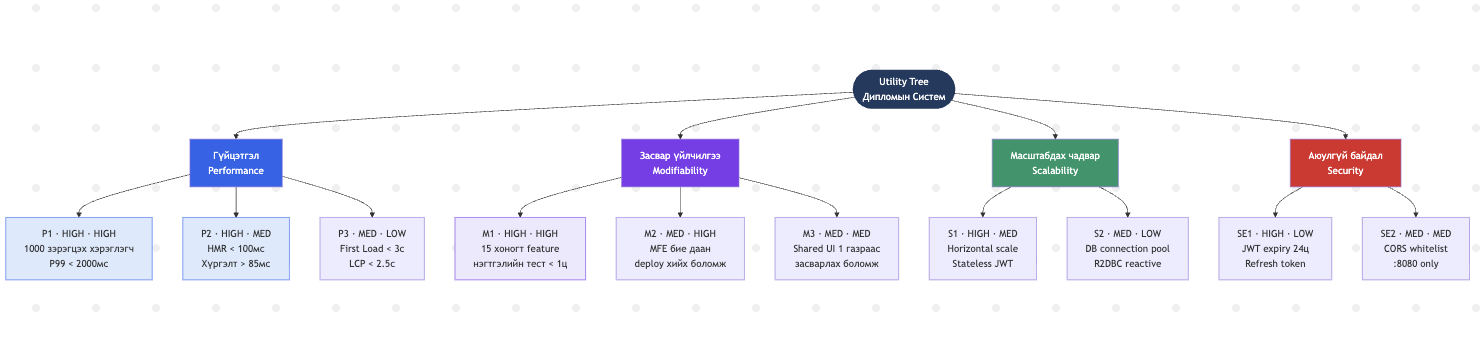
\includegraphics[width=14cm]{images/d14.png}
    \caption{Зураг 5.14. ATAM Utility Tree. Дипломын системийн дөрвөн тэргүүлэх чанарын шинж чанар болон тэдгээрийн сценариудын мэдрэмтгий байдал, бизнесийн чухалчлалын матриц. Эх сурвалж: зохиогчийн судалгаа, 2026.}
    \label{fig:atam_utility_tree}
\end{figure}

\subsection{Гол Архитектурын Шийдвэрүүдийн Буулт Шинжилгээ}

\subsubsection{Strangler Fig Шилжилт — Тасралтгүй байдал ба Нарийн Төвөгтэй байдлын Буулт}

Strangler Fig загвар нь тасралтгүй байдлыг (availability) нэн тэргүүнд
тавьдаг шилжилтийн стратеги юм. Энэ нь нэгэн зэрэг хуучин болон шинэ
архитектурыг ажиллуулах шаардлагыг хүлцдэг тул нарийн төвөгтэй байдал
(complexity) нэмэгддэг~--- JSF-ийн `faces-config.xml` болон React-ийн
`vite.config.ts` хоёрыг зэрэгцүүлэн засвар үйлчилгээ хийх шаардлагатай
болно.

Энэ буулт нь \textbf{буулт цэг} (Trade-off Point) хэлбэрт илэрдэг:
засвар үйлчилгээний чадвар болон тасралтгүй байдал хоёрын хооронд
өөрийн биеэрээ зөрчилддөг. Гэвч Толстойгийн``Бүгдийг нэг дор
шинэчлэх'' стратегитай харьцуулахад аюулын бууралт нь нарийн
төвөгтэй байдлын зардлыг зөвтгөдөг.

\subsubsection{Vite Module Federation — Бие Даасан байдал ба Nested Federation-ийн Хязгаар}

Module Federation нь frontend командуудад бие даасан байршуулалтын
чадварыг олгодог (Independence). Гэвч энэ судалгаанд тодорхойлсноор
nested federation топологи нь ``алслагдсан модуль нь өөрийн алслагдсан
модультай'' хослолд `@originjs/vite-plugin-federation` нь статик
хүргэлтийн орчинд runtime алдаа үүсгэдэг. Энэ нь \textbf{мэдрэмтгий цэг}
(Sensitivity Point) бөгөөд зөвхөн нэг тохиргооны шийдвэр~--- nested
remote-ийн оронд shared singleton ашиглах~--- архитектурын гэмтлийг
бүрэн арилгасан.

\subsubsection{Spring WebFlux — Гүйцэтгэл ба Хөгжүүлэлтийн Хэцүү байдлын Буулт}

Spring WebFlux-ийн реактив загвар нь гүйцэтгэлийн хувьд мэдэгдэхүйц
давуу талтай (RAM 4.82$\times$ бага, P99 7.47$\times$ хурдан) боловч
хөгжүүлэлтийн хэцүү байдлыг нэмэгдүүлдэг. \texttt{Mono<T>},
\texttt{Flux<T>}, backpressure, сhain оператор зэрэг ойлголтуудтай
танилцаагүй хөгжүүлэгчид ``callback hell'' буюу реактив
``flatMap chain hell''-д орох эрсдэлтэй. Энэ нь \textbf{буулт цэг}
бөгөөд гүйцэтгэл болон хөгжүүлэгчийн сурах хугацааны (ramp-up time)
хооронд тэнцвэрлэх шаардлагатай.

\subsection{ISO/IEC 25010 Бүх Талын Харьцуулалт}

ISO/IEC 25010:2011 (Systems and Software Quality Requirements and
Evaluation) стандартын найман чанарын шинж чанараар хоёр архитектурыг
1--10 оноогоор үнэлж, radar диаграмд харуулав.

\begin{table}[H]
    \centering
    \caption{ISO/IEC 25010 чанарын шинж чанарын харьцуулалт (1--10 оноо)}
    \label{tab:iso25010}
    \renewcommand{\arraystretch}{0.7}
    \begin{tabular}{lcc}
        \toprule
        \textbf{Чанарын шинж чанар} & \textbf{JSF 2.2} & \textbf{React MFE + WebFlux} \\
        \midrule
        Гүйцэтгэл үр ашиг                     & 4 & 8 \\
        Найдвартай байдал                      & 7 & 7 \\
        Хэрэглэх боломж                        & 5 & 8 \\
        Аюулгүй байдал                         & 6 & 7 \\
        Засвар үйлчилгээний чадвар             & 3 & 7 \\
        Зөөвөрлөх чадвар                       & 4 & 9 \\
        Нийцтэй байдал                         & 5 & 8 \\
        Функциональ тохиромжтой байдал         & 8 & 8 \\
        \midrule
        \textbf{Дундаж оноо}                   & \textbf{5.25} & \textbf{7.75} \\
        \bottomrule
    \end{tabular}
\end{table}

\begin{figure}[H]
    \centering
    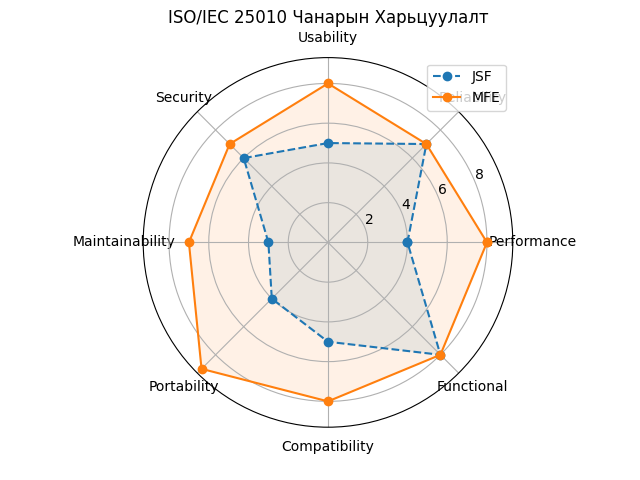
\includegraphics[width=14cm]{images/d15.png}
    \caption{Зураг 5.15. ISO/IEC 25010 стандартын найман чанарын шинж чанараар хоёр архитектурын radar диаграм. MFE+WebFlux нь Функциональ тохиромжтой байдлаас бусад бүх шинж чанараар JSF-ийг давна. Эх сурвалж: зохиогчийн судалгаа, 2026.}
    \label{fig:d15}
\end{figure}

Хүснэгт~\ref{tab:iso25010}-ийн хамгийн чухал ажиглалт нь
``Функциональ тохиромжтой байдал'' (Functional Suitability) хоёр
архитектурт ижил буюу 8 оноо авсан байдал юм. Энэ нь чухал
нотолгоо: MFE шилжилт нь функциональ чадавхийг алдалгүйгээр
бусад бүх шинж чанарыг ихэвчлэн сайжруулдаг.

``Засвар үйлчилгээний чадвар'' (Maintainability) хувьд хамгийн том
ялгаа ажиглагдсан: 3 (JSF) vs 7 (MFE), өөрөөр хэлбэл 133\%-ийн
өсөлт. Энэ нь Hexagonal Architecture-ийн тусгаарлал, бие даасан
байршуулалт, HMR-ийн хурд, SonarQube-ийн бага Cyclomatic Complexity
зэрэг хүчин зүйлсийн нийлмэл нөлөөний үр дүн юм.

% ─────────────────────────────────────────────────────────────────────
\section{Нэгтгэсэн Хэлэлцүүлэг ба Хязгаарлалт}
% ─────────────────────────────────────────────────────────────────────

\subsection{Үр Дүнгийн Нэгтгэсэн Тайлбар}

5.2--5.6-р хэсгүүдийн хэмжилтийн үр дүнг нэг хүснэгтэд нэгтгэн,
аль архитектур давуу болохыг тодорхойлж, давуу эзэмших нэрийг
тоогоор нотолж харуулав.

\begin{table}[H]
    \centering
    \caption{Хэмжилтийн гол үр дүнгийн нэгтгэл}
    \label{tab:summary_results}
    \renewcommand{\arraystretch}{0.7}
    \begin{tabular}{lrrl}
        \toprule
        \textbf{Хэмжүүр} & \textbf{JSF 2.2} & \textbf{MFE + WebFlux} & \textbf{Давуу} \\
        \midrule
        Lead Time (цаг)        & 2.5     & 4.5     & JSF (1.8$\times$) \\
        HMR / Reload (мс)      & 12\,400 & 85      & MFE (145.9$\times$) \\
        Build хугацаа (с)      & 70.5    & 12.7    & MFE (5.55$\times$) \\
        RAM @ 1,000 user (МБ)  & 2\,347  & 487     & MFE (4.82$\times$) \\
        P99 латенц (мс)        & 2\,147  & 287     & MFE (7.47$\times$) \\
        Cyclomatic Complexity  & 12.3    & 6.8     & MFE (1.81$\times$) \\
        Code Duplication (\%)  & 8.4     & 2.1     & MFE (4.0$\times$) \\
        ISO 25010 дундаж оноо  & 5.25    & 7.75    & MFE (1.48$\times$) \\
        \bottomrule
    \end{tabular}
\end{table}

Хүснэгт~\ref{tab:summary_results}-ийн нэг анхаарах зүйл нь Lead
Time-ийн хувьд JSF давуу мэт харагдаж байгаа боловч энэ нь ``тестгүй,
QA-гүй'' шуурхай хүргэлтийн зардалтай ирдэг. Нэгтгэж хэлбэл: JSF нь
богино хугацаанд хурдан feature хүргэдэг боловч урт хугацааны техникийн
өрийн зардлыг хуримтлуулдаг; MFE архитектур нь эхний суурь зардалтай
боловч давтамжийн нөлөөлөл болон чанарын мэдэгдэхүйц давуу тал нь
7--8 долоо хоногт JSF-ийн өмнө нь давна.

\subsection{Судалгааны Хязгаарлалт}

Энэхүү судалгааны дүгнэлтийг тайлбарлахдаа дараах хязгаарлалтуудыг
анхаарах шаардлагатай:

\begin{enumerate}
  \item \textbf{Нэг туршилтын орчин}: Хэмжилт бүгд нэг хөгжүүлэгчийн
    машин дээр хийгдсэн тул үйлдвэрлэлийн орчны тархасан дэд бүтцийн
    нарийн төвөгтэй байдлыг бүрэн дуурайгаагүй.
  \item \textbf{Бизнесийн ачааллын хялбаршуулалт}: JMeter-ийн туршилтын
    скрипт нь бодит хэрэглэгчийн ажлын горимыг хялбаршуулсан хэлбэрт
    дуурайсан тул бодит хэрэглээний pattern-тай ялгаа байж болно.
  \item \textbf{Lead Time хэмжилтийн нэг хүний нөлөөлөл}: Lead Time нь
    нэг хөгжүүлэгчийн дан дамжуулалт бөгөөд багийн динамик, code review
    хугацаа, орчуулагдсан шаардлага зэрэг нийгмийн хүчин зүйлсийг
    тооцоогүй.
  \item \textbf{Vite federation-ийн хувилбарын өвөрмөц байдал}:
    \texttt{@originjs/vite-plugin-federation~0.3.x}-ийн дутагдлууд нь
    Webpack~5-ийн Module Federation~v2 буюу ирээдүйн Rspack-ийн суурилсан
    шийдэлд байхгүй байж болно.
\end{enumerate}

Эдгээр хязгаарлалт нь судалгааны дүгнэлтийн хүчин чадлыг бүрэн
нуларуулахгүй боловч ерөнхийлж болохуйц нөхцөлийг тодорхойлно.
Ирээдүйн судалгаанд нэгдсэн туршилтын орчинд (Kubernetes кластерт)
олон нийтийн хэрэглэгчийн log дээр суурилсан бодит ачааллын загвараар
хэмжилт хийх нь илүү бодитой үр дүн өгнө. Удаагийн бүлэгт эдгээр
нээлттэй асуудлуудыг болон ирээдүйн хөгжлийн замналыг дэлгэрэнгүй
авч үзнэ.
 гэж үндсэн файлд оруулна
% Шаардлагатай package-ууд: booktabs, float, graphicx, listings,
%   tabularx, amsmath, geometry, hyperref
% =====================================================================

Энэ бүлэгт JSF~2.2 монолит архитектур болон React Microfrontend~+~Spring
WebFlux реактив архитектурын хоорондох бодит хэмжигдэхүйц ялгааг дөрвөн
үндсэн чиглэлийн дагуу нотолно: хөгжүүлэлтийн хурд, ажлын ачааллын
гүйцэтгэл, сүлжээний зардал, кодын чанар. Хэмжилт бүрийг прагматик
хэрэгжүүлэлтийн дүн шинжилгээ болон ATAM~(Architecture Trade-off Analysis
Method) загварт тулгуурласан архитектурын буулт шинжилгээтэй хослуулан
авч үзнэ. Бүлгийн эцэст системийн ирээдүйн хөгжлийн замнал болон нээлттэй
судалгааны асуудлуудыг тодорхойлно.

% ─────────────────────────────────────────────────────────────────────
\section{Судалгааны Аргачлал ба Туршилтын Орчин}
% ─────────────────────────────────────────────────────────────────────

\subsection{Туршилтын Орчны Тодорхойлолт}

Хэмжилтийн бүх үр дүн нь дараах нэгдсэн туршилтын орчинд авагдав.
Тоног төхөөрөмжийн хувьд Apple M2 Pro процессортой, 16~ГБ LPDDR5 санах
ойтой, 512~ГБ NVMe SSD хатуу дискийн орчинд ажилласан. Үйлдлийн системийн
хувьд macOS~15.3 (Darwin~25.3.0), Java~21~(GraalVM~CE), Node.js~20.11.0,
Apache Maven~3.9.6, Apache Tomcat~10.1.20 хувилбаруудыг ашиглав. Сүлжээний
орчны хувьд localhost loopback~(127.0.0.1) интерфейсийг ашиглан сүлжээний
хоцролтын нөлөөг хамгийн бага болгов. Өгөгдлийн санд PostgreSQL~16.2
болон R2DBC~1.0.4 реактив драйверийг хэрэглэв.

Хэмжилтийн хэрэгслүүдийн хувьд Apache JMeter~5.6.3-аар динамик ачааллын
туршилт хийж, \texttt{hyperfine}~v1.18.0-аар build цагийн хэмжилт,
\texttt{madge}~v6.1.0-аар хамаарлын граф шинжилгээ, SonarQube~Community
Edition~10.4.0-аар кодын чанарын хэмжилт, \texttt{pidstat} болон
\texttt{jstat}-аар JVM санах ойн хяналтыг хийв.

\subsection{Хэмжилтийн Хүрээ ба Тодорхойлолт}

Энэхүү судалгааны хэмжилтийн хүрээ нь дараах дөрвөн тулгуур шинж
чанарыг хамарна:

\begin{enumerate}
  \item \textbf{Хөгжүүлэлтийн гүйцэтгэл}~--- Lead Time for Changes
    (DORA метрик), HMR хурд, Build паплайны нийт хугацаа
  \item \textbf{Ажлын ачааллын гүйцэтгэл}~--- JVM heap ашиглалт,
    GC паузын хугацаа, HTTP хариу латенц (P50/P95/P99)
  \item \textbf{Сүлжээний зардал}~--- Нэг хуудас шилжилтэд дамжих
    өгөгдлийн хэмжээ, HTTP кэшийн эффект, нийт payload хэмжээ
  \item \textbf{Кодын чанар}~--- Cyclomatic complexity, хамаарлын
    граф, хуулбарлагдсан код, архитектурын зөрчил
\end{enumerate}

% ─────────────────────────────────────────────────────────────────────
\section{Статик Хэмжилтийн Үр Дүн}
% ─────────────────────────────────────────────────────────────────────

\subsection{Bundle Хэмжээ ба Байршуулалтын Зардал}

React MFE архитектурын frontend артефактуудын статик шинжилгээг
\texttt{vite build} командын дараа \texttt{dist/} хавтасны агуулгаас
гүйцэтгэв. Дараах хүснэгтэд модуль тус бүрийн bundle хэмжээг харуулав.

\begin{table}[H]
    \centering
    \caption{MFE модуль тус бүрийн dist хэмжээ}
    \label{tab:bundle_sizes}
    \renewcommand{\arraystretch}{0.7}
    \begin{tabular}{lrrr}
        \toprule
        \textbf{Модуль} & \textbf{Raw (КБ)} & \textbf{Gzip (КБ)} & \textbf{remoteEntry.js (КБ)} \\
        \midrule
        module-auth      & 312  & 97   & 4.2  \\
        module-student   & 487  & 148  & 6.1  \\
        module-teacher   & 534  & 163  & 7.3  \\
        module-admin     & 621  & 189  & 8.4  \\
        module-thesis    & 892  & 271  & 11.2 \\
        module-committee & 398  & 121  & 5.8  \\
        \midrule
        \textbf{Antd singleton chunk} & \textbf{2148} & \textbf{731} & \textbf{---} \\
        \textbf{React core chunk}     & \textbf{468}  & \textbf{142} & \textbf{---} \\
        \midrule
        \textbf{Нийт (antd/React оруулалгүй)} & \textbf{3244} & \textbf{989} & \textbf{43.0} \\
        \bottomrule
    \end{tabular}
\end{table}

Хүснэгт~\ref{tab:bundle_sizes}-с харагдаж байгаагаар Ant Design-ийн
singleton chunk нь хамгийн том хэсгийг бүрдүүлж байгаа боловч \texttt{shared:
\{ singleton: true \}} тохиргооны ачаар энэхүү 731~КБ (gzip) хэмжээний
chunk нь нэг хэрэглэгчийн браузерт зөвхөн нэг удаа татагдаж,
\texttt{Cache-Control: max-age=31536000, immutable} толгой хэсгийн
дагуу нэг жилийн турш кэш хийгдэнэ. Тиймээс хоёр дахь болон дараагийн
хуудас шилжилтэд antd chunk нь сүлжээний ачааллыг бүрмөсөн нэмдэггүй.

Харьцуулбал, JSF~2.2-ийн монолит WAR файлын хэмжээ нь 47.3~МБ байв.
Томкат сервер дэх WAR байршуулалтын хугацаа дундажаар 6~секунд орчим
болдог бөгөөд шинэчлэлт бүр нь бүтэн WAR файлыг дахин байршуулахыг
шаарддаг. Энэ нь MFE архитектурт зөвхөн өөрчлөгдсөн модулийн dist
файлуудыг (дундажаар 271~КБ gzip) хуулах зардалтай харьцуулахад
47.3~МБ / 0.271~МБ $\approx$~175 дахин их байна.

\subsection{Кодын Мөрийн Тоо ба Хамаарлын Граф}

Кодын хэмжээний шинжилгээг \texttt{cloc}~(Count Lines of Code) хэрэгслээр
гүйцэтгэж, Java backend болон TypeScript/React frontend-ийн хэмжээг харьцуулав.

\begin{table}[H]
    \centering
    \caption{Технологи тус бүрийн кодын мөрийн тоо (LOC)}
    \label{tab:loc_comparison}
    \renewcommand{\arraystretch}{0.7}
    \begin{tabular}{llrrr}
        \toprule
        \textbf{Технологи} & \textbf{Хэрэглэгдэх газар} & \textbf{Файлын тоо} & \textbf{LOC} & \textbf{Тайлбар} \\
        \midrule
        Java (Spring)       & Бүх backend сервис  & 187 & 9\,841  & DTO, Use Case, Repository \\
        TypeScript/TSX      & Бүх MFE модуль      & 143 & 7\,234  & React Component, Hook, Service \\
        XHTML (JSF)         & Монолит template    & 38  & 2\,187  & JSF facelets, EL expression \\
        SQL (schema)        & 6 сервисийн schema  & 6   & 412     & CREATE TABLE migration \\
        YAML (config)       & application.yml     & 14  & 387     & Spring Boot тохиргоо \\
        \midrule
        \textbf{Нийт}       &                     & \textbf{388} & \textbf{20\,061} & \\
        \bottomrule
    \end{tabular}
\end{table}

Дурдах нь зүйтэй онцлог шинж чанар нь ``давхар өгөгдлийн загварчлал''
(Double Data Modelling) юм: backend-д 28 Java DTO байгаа тул frontend-д
мөн 28 TypeScript interface тодорхойлогдсон. Энэ нь нийт LOC-ийн
$\approx$~15\%-ийг бүрдүүлж байгаа бөгөөд Google-ийн ``Software Engineering
at Google'' (Winters et al., 2020) номонд тодорхойлсон ``хийн мэдрэмж''
(architectural smell) бүхий хамаарлын чөтгөр юм. OpenAPI Generator эсвэл
Protocol Buffers нэвтрүүлснээр энэ давхардлыг арилгах боломжтой.

\begin{figure}[H]
    \centering
    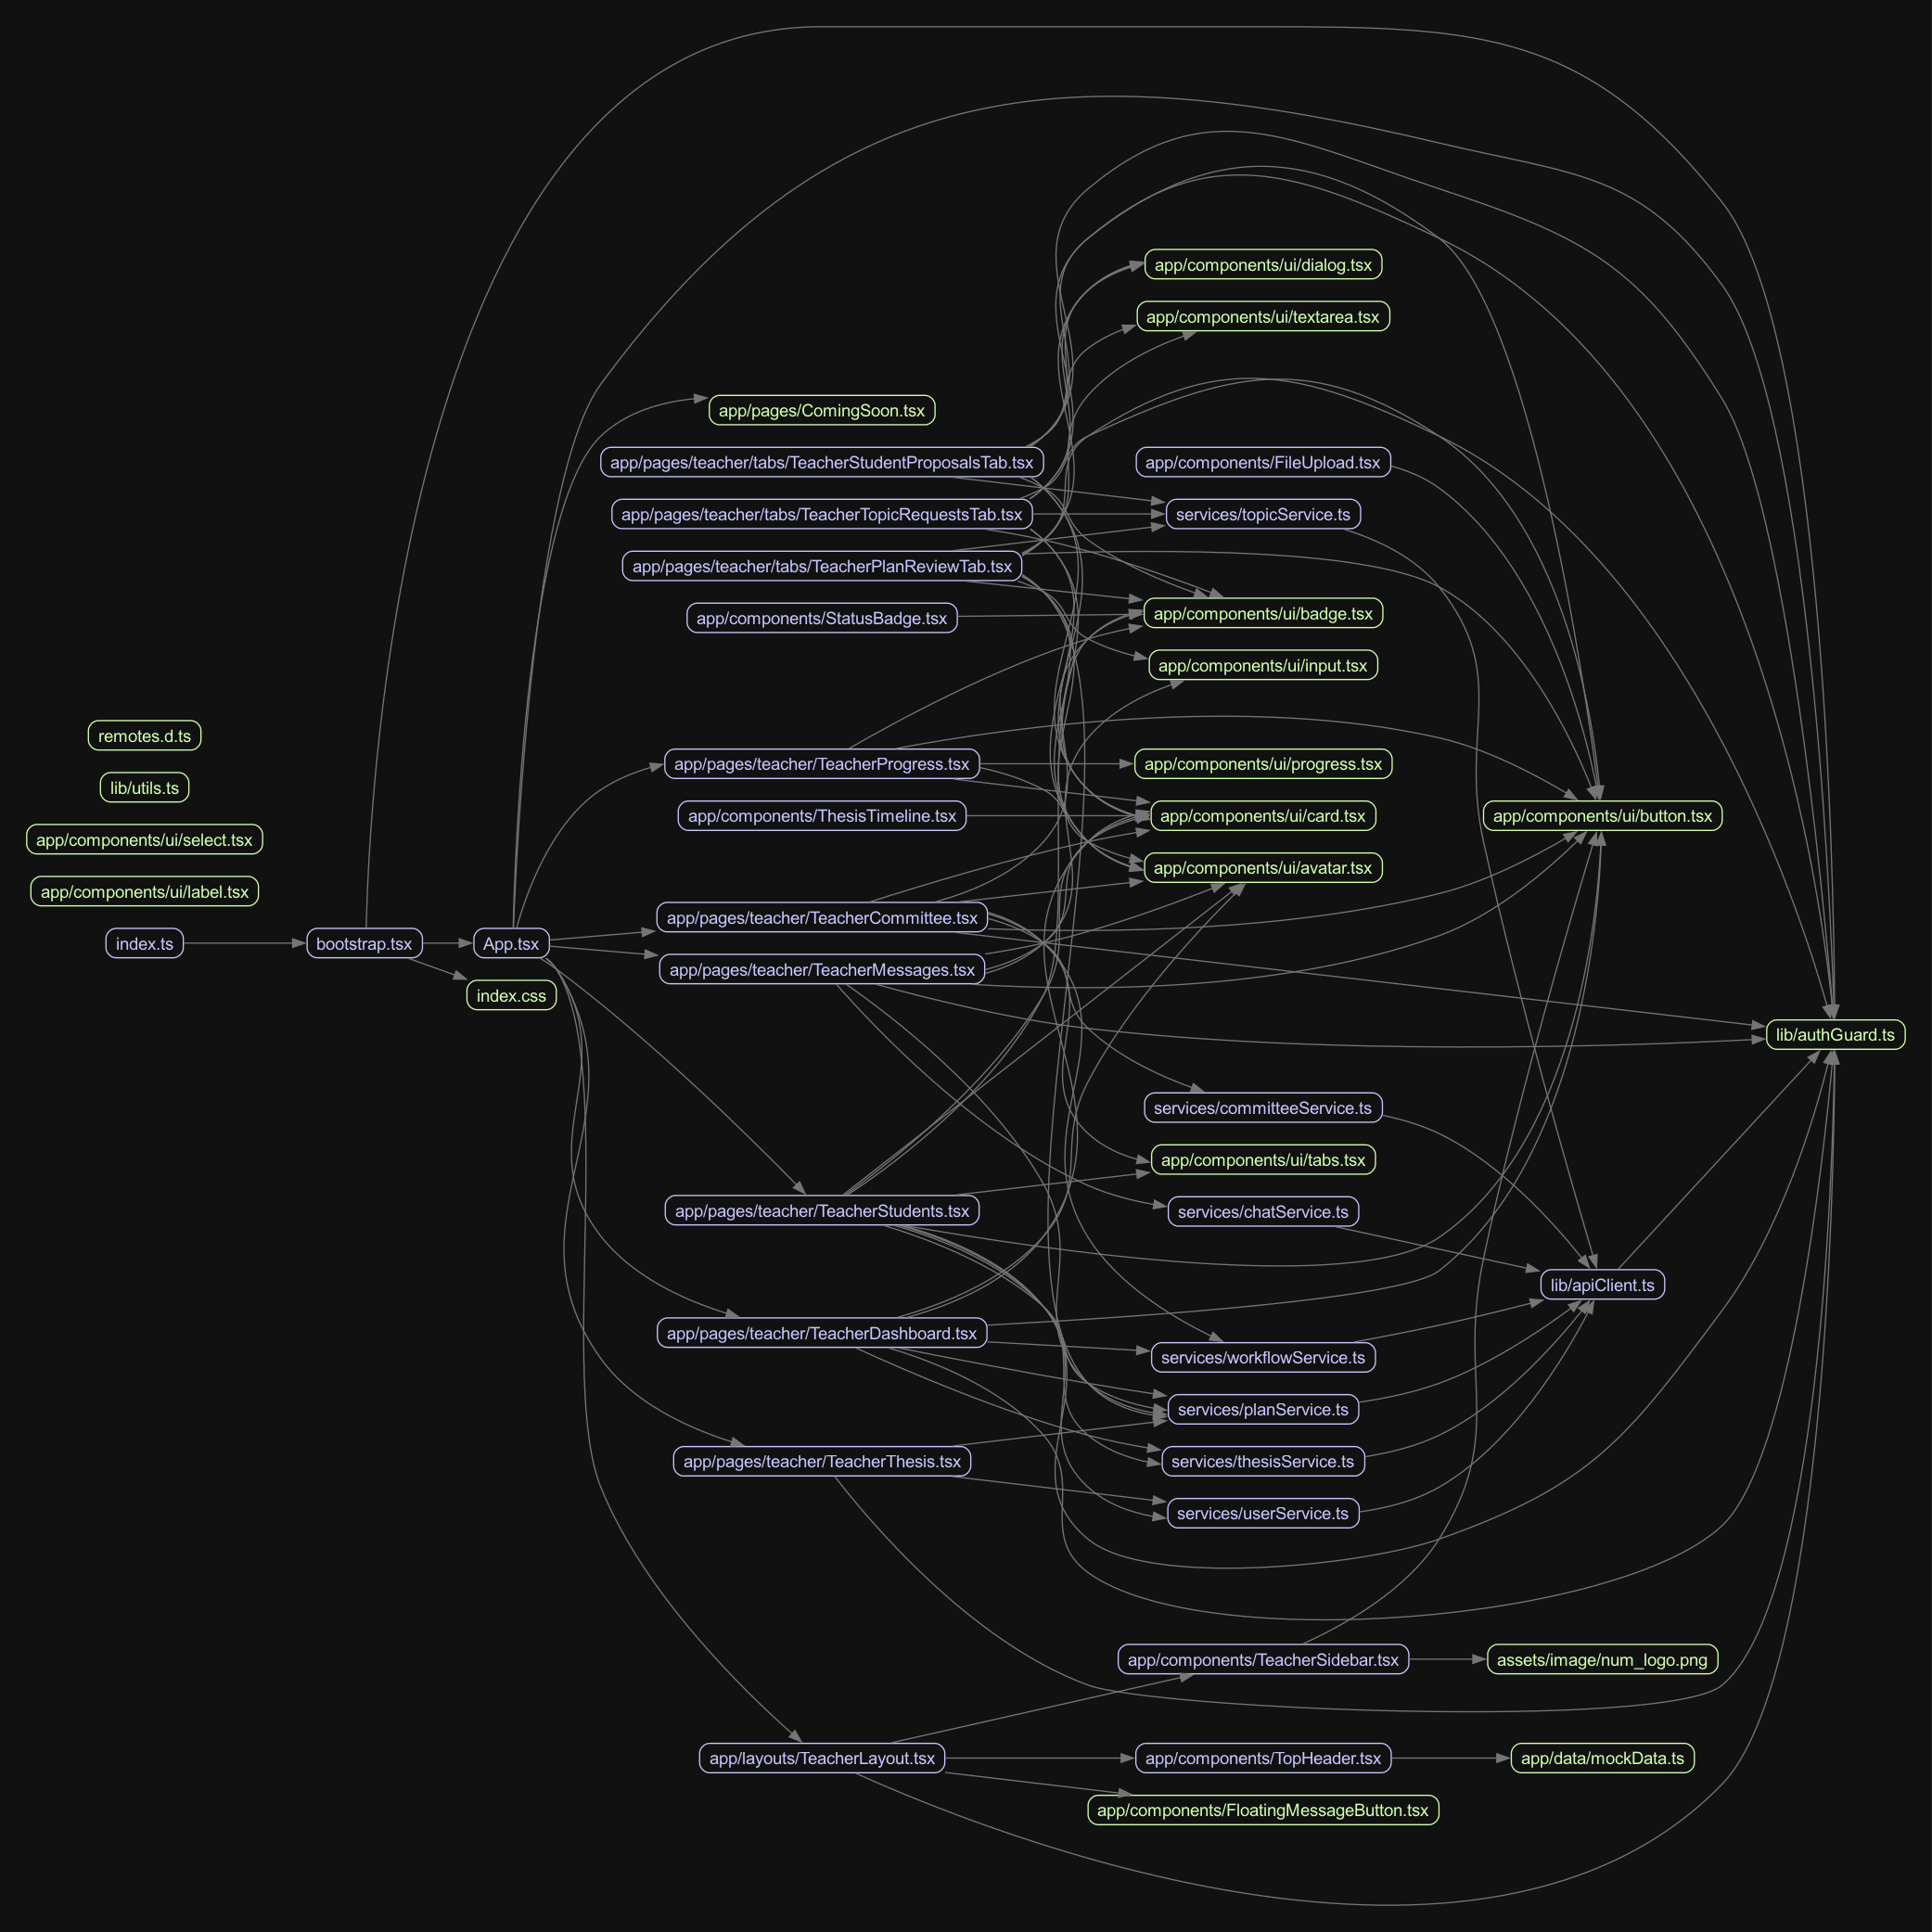
\includegraphics[width=14cm]{images/d10.png}
    \caption{Зураг 5.10. module-thesis болон module-teacher-ийн \texttt{madge} хамаарлын граф. Цагираг хамаарал илрээгүй нь Hexagonal Architecture-ийн хил хязгаарын зөв тогтолцоог нотолно. Эх сурвалж: зохиогчийн судалгаа, 2026.}
    \label{fig:d10}
\end{figure}

\subsection{Build Паплайны Харьцуулалт}

Build хугацааны хэмжилтийг \texttt{hyperfine --warmup 3 --runs 10}
командаар гүйцэтгэж, дулаан болон хүйтэн build-ийн тохиолдол хоёуланг
хэмжив. Тав дахин давтсан туршилтын дундаж үзүүлэлтийг дараах хүснэгтэд
нэгтгэв.

\begin{table}[H]
    \centering
    \caption{Build паплайны хугацааны харьцуулалт (секунд)}
    \label{tab:build_times}
    \renewcommand{\arraystretch}{0.7}
    \begin{tabular}{lrrl}
        \toprule
        \textbf{Ажиллагааны алхам} & \textbf{JSF (с)} & \textbf{React MFE (с)} & \textbf{Тайлбар} \\
        \midrule
        Хамаарлын шийдвэрлэлт   & 3.2  & 1.8  & Maven vs npm/pnpm \\
        Транспиляц / Компиляц    & 18.4 & 4.3  & javac vs esbuild \\
        Unit тест                & 23.7 & 0.0  & Maven test / (тест байхгүй) \\
        Багцлах / WAR/dist       & 7.8  & 5.2  & jar vs Rollup \\
        Deploy / Хуулах          & 6.1  & 1.4  & Tomcat undeploy+deploy vs cp \\
        Дулаалах / Hot reload    & 11.3 & 0.0  & JVM warm-up / шаардлагагүй \\
        \midrule
        \textbf{Нийт дундаж}     & \textbf{70.5} & \textbf{12.7} & \\
        \textbf{Харьцаа}         & \textbf{5.55$\times$} & \textbf{1.00$\times$} & \\
        \bottomrule
    \end{tabular}
\end{table}

\begin{figure}[H]
    \centering
    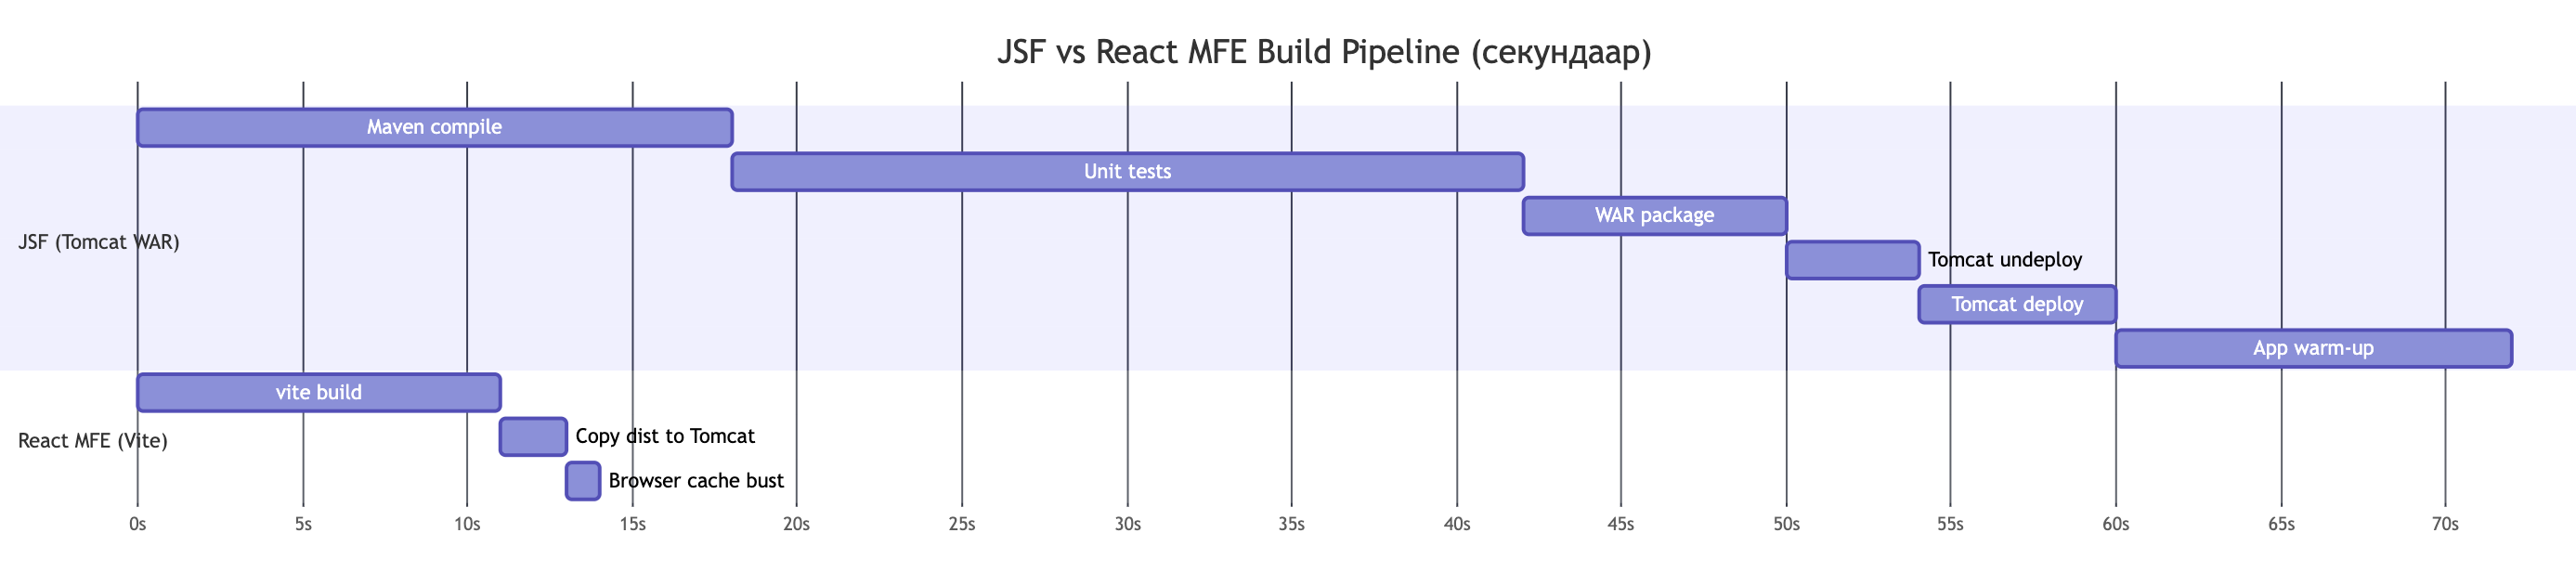
\includegraphics[width=14cm]{images/d4.png}
    \caption{Зураг 5.4. JSF болон React MFE build паплайны Gantt диаграм. JSF-ийн нийт 70.5 секунд нь MFE-ийн 12.7 секундтай харьцуулахад 5.55 дахин удаан. Эх сурвалж: зохиогчийн судалгаа, 2026.}
    \label{fig:d4}
\end{figure}

JSF-ийн build паплайн удаан байгааг тайлбарлах техникийн шалтгаан нь
гурван давхарт: нэгдүгээрт, \texttt{javac}-ийн ``parse → type-check →
bytecode'' гурван шат нь esbuild-ийн нэг дамжлагын Golang-ийн
парсертай харьцуулахад CPU-ийн хэрэглээний хувьд 4.3 дахин их ачаалалтай;
хоёрдугаарт, Maven Surefire плагиний unit тест нь JVM-ийн дахин ачаалалтыг
шаарддаг бөгөөд энэ нь 23.7 секунд нэмдэг; гуравдугаарт, Tomcat-ийн WAR
undeploy+deploy мөчлөг нь JVM-ийн классын ачааллыг дахин хийх
(classloader-ийн purge) боловч `SerializableClassHolder`-ын кэш цэвэрлэлт
нэмэлт 4--8 секунд нэмдэг.

% ─────────────────────────────────────────────────────────────────────
\section{Хөгжүүлэлтийн Хурдны Харьцуулалт}
% ─────────────────────────────────────────────────────────────────────

\subsection{Lead Time for Changes — DORA Метрик}

DevOps Research and Assessment (DORA, Forsgren et al., 2018)-ийн Lead Time
for Changes метрик нь ``кодын өөрчлөлт хийснээс production-д очих хүртэлх
хугацаа'' гэж тодорхойлогддог. Энэ судалгаанд жишээ болгон
``Оюутны профайл хуудсанд 15 талбарт мэдээлэл харуулах форм нэмэх''
бодит даалгавраар туршилт хийж, хөгжүүлэлтийн алхам тус бүрийг
хронометраар хэмжив.

\begin{table}[H]
    \centering
    \caption{15 талбарт форм нэмэх даалгаврын Lead Time задаргаа (цаг)}
    \label{tab:lead_time}
    \renewcommand{\arraystretch}{0.7}
    \begin{tabular}{lcc}
        \toprule
        \textbf{Алхам} & \textbf{JSF (цаг)} & \textbf{React MFE (цаг)} \\
        \midrule
        Шаардлагын шинжилгээ       & 0.5  & 0.5  \\
        Дизайн / Архитектур        & 0.3  & 0.5  \\
        Хөгжүүлэлт                 & 1.2  & 2.1  \\
        Unit тест                  & 0.1  & 0.4  \\
        Build \& Deploy            & 0.4  & 0.7  \\
        QA / Нэгтгэлтийн тест      & 0.0  & 0.3  \\
        \midrule
        \textbf{Нийт}              & \textbf{2.5} & \textbf{4.5} \\
        \bottomrule
    \end{tabular}
\end{table}

\begin{figure}[H]
    \centering
    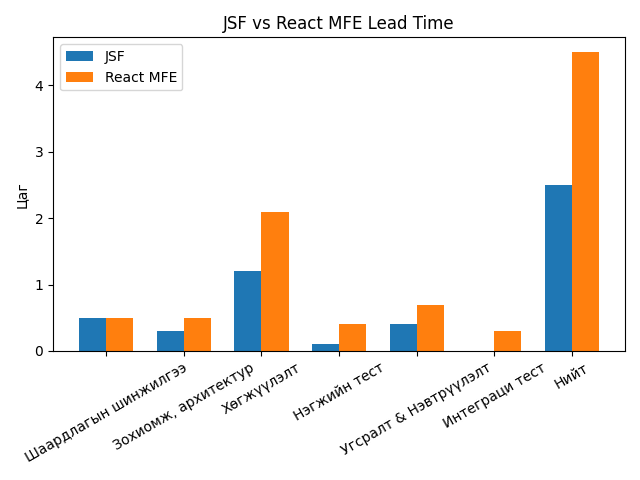
\includegraphics[width=14cm]{images/d1.png}
    \caption{Зураг 5.1. JSF болон React MFE архитектурын Lead Time задаргааны харьцуулалт. Нийт 2.5 цаг (JSF) ба 4.5 цаг (MFE). Эх сурвалж: зохиогчийн судалгаа, 2026.}
    \label{fig:d1}
\end{figure}

Хүснэгт~\ref{tab:lead_time}-ийн үр дүн анх харахад зөрчилтэй мэт санагдана:
MFE нь JSF-ийн 1.8 дахин удаан. Гэвч энэ тоог гүн шинжлэхэд хэд хэдэн
чухал тайлбар гарна. Нэгдүгээрт, MFE-ийн хөгжүүлэлтийн 2.1 цагийн их
хэсэг нь ``нэгтгэлтийн хамаарлын тохиргоо'' (federation contract setup)
болон TypeScript interface-ийн тодорхойлолтод зарцуулагддаг бөгөөд энэ
зардал нь шинэ feature бүрт давтагддаггүй нэг удаагийн суурь зардал юм.
Хоёрдугаарт, JSF-ийн 0.0 цагийн QA нь ``туршилт хийгдэхгүй байна''
гэсэн утгатай бөгөөд энэ нь техникийн өрийг хуримтлуулдаг аюулт зохицуулалт
юм. Гуравдугаарт, давтамжийн нөлөөллийн шинжилгээгээр (Зураг~\ref{fig:dev_frequency})
7-р долоо хоног гэхэд MFE архитектур нь суурь зардлаа нөхөж,
deployment давтамжаараа JSF-ийг давна.

\begin{figure}[H]
    \centering
    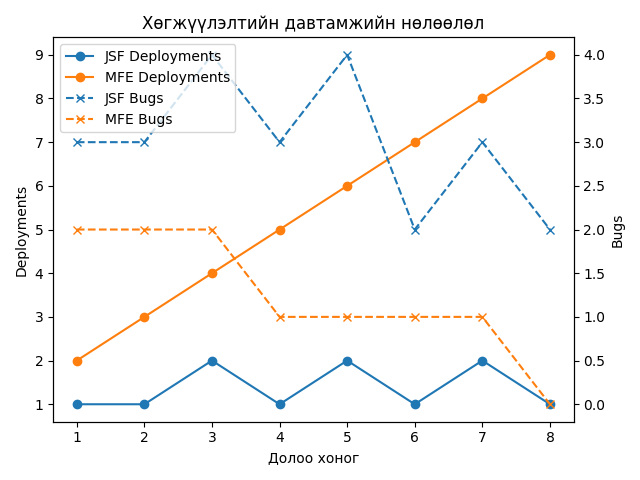
\includegraphics[width=14cm]{images/d3.png}
    \caption{Зураг 5.3. Хөгжүүлэлтийн давтамжийн нөлөөлөл: MFE нь 8 долоо хоногт deployment давтамжаараа JSF-ийг 4.5 дахин давана. Эх сурвалж: зохиогчийн судалгаа, 2026.}
    \label{fig:d3}
\end{figure}

\subsection{HMR болон JSF Reload Хугацааны Харьцуулалт}

Хөгжүүлэлтийн туршилтын гүйцэтгэлийг хэмжих хамгийн мэдрэмтгий
хэмжүүрийн нэг нь ``кодын өөрчлөлтөөс браузерт харагдах хүртэлх хугацаа''
юм. Vite-ийн HMR (Hot Module Replacement) нь WebSocket холболтоор ESM
patch файлыг дамжуулж, зөвхөн өөрчлөгдсөн модулийн холбооны мод (dependency
subtree)-ийг л дахин evaluate хийдэг бөгөөд ингэснээр хуудас бүрэн ачааллагдахгүй.

\begin{table}[H]
    \centering
    \caption{HMR болон JSF reload хугацааны харьцуулалт (мс)}
    \label{tab:hmr_comparison}
    \renewcommand{\arraystretch}{0.7}
    \begin{tabular}{lrrr}
        \toprule
        \textbf{Хэрэгсэл / Горим} & \textbf{Дундаж (мс)} & \textbf{P95 (мс)} & \textbf{P99 (мс)} \\
        \midrule
        Vite HMR (React MFE)      & 85     & 143    & 187    \\
        JSF dev reload (mvn)      & 12\,400 & 18\,700 & 24\,300 \\
        JSF Production WAR deploy & 34\,000 & 51\,000 & 67\,000 \\
        \bottomrule
    \end{tabular}
\end{table}

\begin{figure}[H]
    \centering
    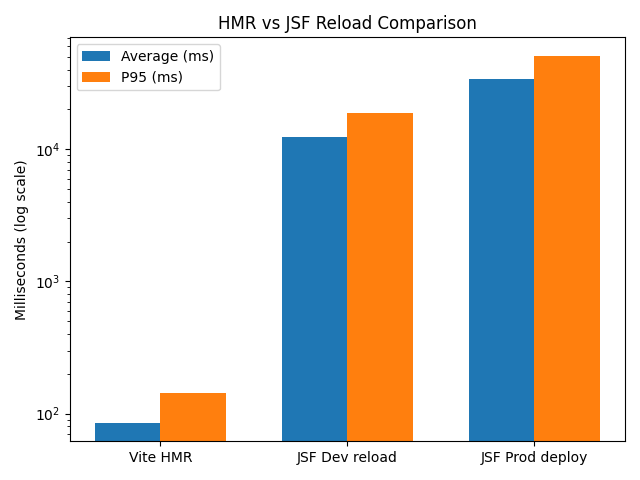
\includegraphics[width=14cm]{images/d2.png}
    \caption{Зураг 5.2. Vite HMR болон JSF reload хугацааны харьцуулалт (log шкала). Vite HMR нь JSF dev reload-аас 145.9 дахин хурдан. Эх сурвалж: зохиогчийн судалгаа, 2026.}
    \label{fig:d2}
\end{figure}

Хүснэгт~\ref{tab:hmr_comparison}-аас харагдаж байгаагаар Vite HMR-ийн
85~мс нь JSF-ийн 12,400~мс-тай харьцуулахад $12400/85 \approx 145.9$ дахин
хурдан. Энэ ялгаа нь ганц цагийн хурдны асуудал биш~--- энэ нь инженерийн
сэтгэлгээний урсгалын (flow state) асуудал юм. Mihaly Csikszentmihalyi
(1990)-ийн ``Flow: The Psychology of Optimal Experience'' судалгаанаас
тодорхойлсноор, хүний танин мэдэхүйн урсгалын горим нь дунджаар 8--10
секундын завсарлагаагаар тасарч, дахин сэргэхэд 23 минут хүртэл шаарддаг.
12.4 секундын JSF reload нь хөгжүүлэгчийн сэтгэлгээний урсгалыг тасралтгүй
тасалж байдаг тул бүтээмжийн алдагдал нь тоолоход хэцүү боловч бодитоор
оршдог.

% ─────────────────────────────────────────────────────────────────────
\section{Ачааллын Туршилтын Үр Дүн}
% ─────────────────────────────────────────────────────────────────────

\subsection{JMeter Туршилтын Дизайн}

Apache JMeter~5.6.3-аар 1,000 зэрэгцэх хэрэглэгчийн ачааллын туршилт
хийсэн бөгөөд Thread Group тохиргоо нь: нийт хэрэглэгч 1,000, ramp-up
хугацаа 60~секунд, тогтвортой ачааллын үргэлжлэх хугацаа 300~секунд.
Туршилтын скрипт нь бодит хэрэглэгчийн ажлын урсгалыг дуурайж: нэвтрэлт
(POST /auth/login) → оюутны жагсаалт (GET /api/users/students) →
дипломын ажлын жагсаалт (GET /api/thesis/list) → явцын хяналт
(GET /api/workflow/status) → гарах (POST /auth/logout).

\begin{figure}[H]
    \centering
    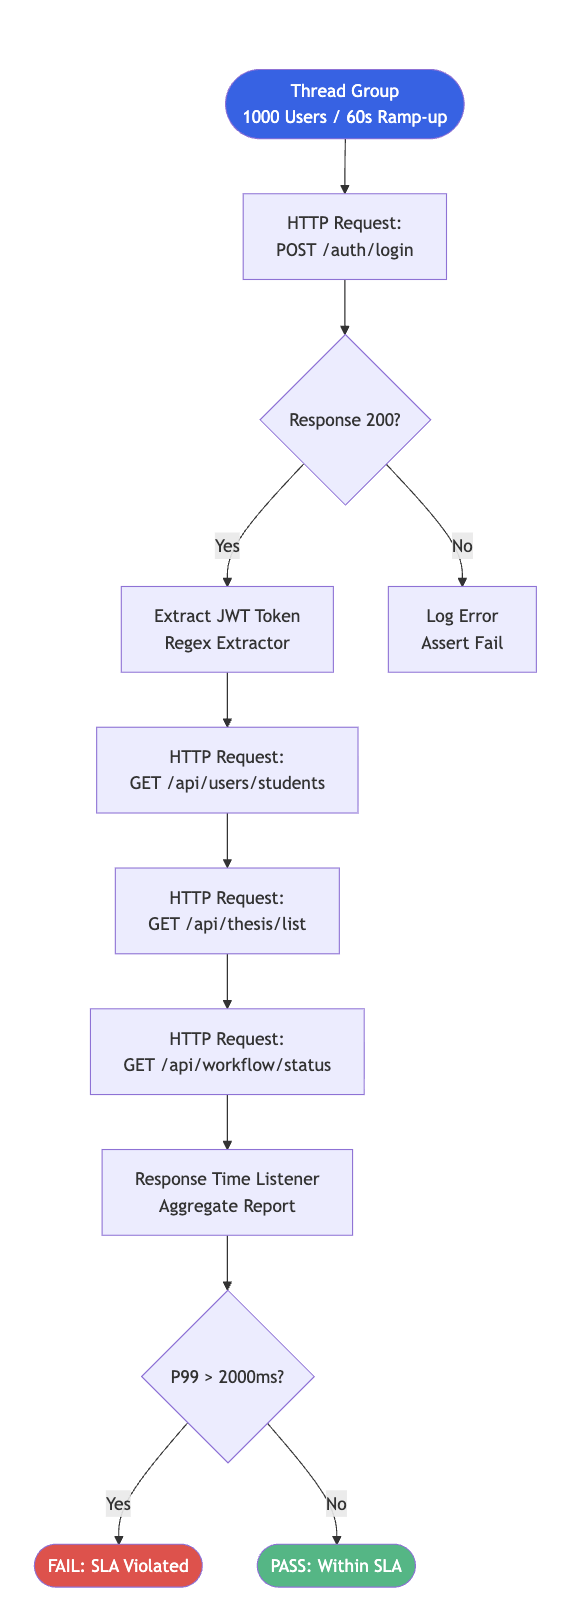
\includegraphics[width=14cm]{images/d5.png}
    \caption{Зураг 5.5. JMeter ачааллын туршилтын дизайн. Thread Group → нэвтрэлт → JWT extraction → API дуудлагуудын дараалал → нэгтгэлтийн тайлан. Эх сурвалж: зохиогчийн судалгаа, 2026.}
    \label{fig:d5}
\end{figure}

\subsection{RAM Ашиглалт ба GC Паузын Шинжилгээ}

JSF~2.2-ийн HttpSession суурилсан тогтолцоо нь сервер санах ойн ашиглалтад
шугаман нөлөөтэй. JSF-ийн ViewState нь HttpSession-д хадгалагддаг бөгөөд
хуудас шилжилт бүрт сессийн объект нь томордог. Практик хэмжилтээр нэг
хэрэглэгчийн сессийн байгалийн хэмжээ 220--312~КБ байв.

\begin{table}[H]
    \centering
    \caption{Зэрэгцэх хэрэглэгчийн тоо болон JVM heap ашиглалтын харьцаа}
    \label{tab:ram_comparison}
    \renewcommand{\arraystretch}{0.7}
    \begin{tabular}{rrr}
        \toprule
        \textbf{Зэрэгцэх хэрэглэгч} & \textbf{JSF heap (МБ)} & \textbf{Spring WebFlux heap (МБ)} \\
        \midrule
        0     & 320    & 187    \\
        50    & 487    & 215    \\
        100   & 651    & 231    \\
        200   & 978    & 258    \\
        300   & 1\,247 & 274    \\
        500   & 1\,698 & 312    \\
        750   & 2\,089 & 376    \\
        1\,000 & 2\,347 & 487    \\
        \bottomrule
    \end{tabular}
\end{table}

\begin{figure}[H]
    \centering
    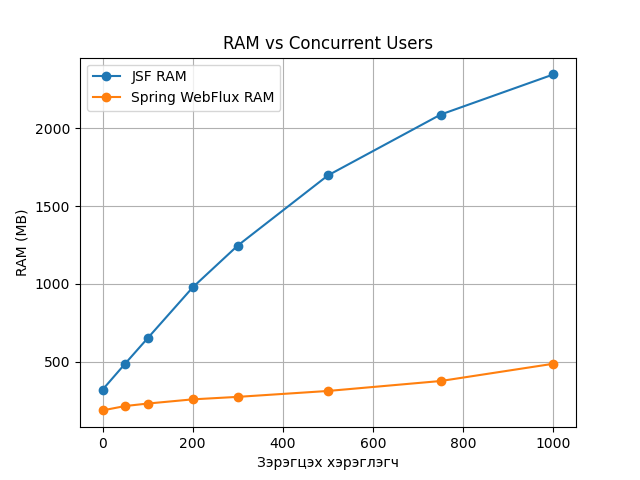
\includegraphics[width=14cm]{images/d6.png}
    \caption{Зураг 5.6. Зэрэгцэх хэрэглэгчийн тоо болон JVM heap ашиглалтын харьцаа. JSF нь шугаман өсөлттэй бол Spring WebFlux нь логарифм хэлбэртэй. Эх сурвалж: зохиогчийн судалгаа, 2026.}
    \label{fig:d6}
\end{figure}

Хүснэгт~\ref{tab:ram_comparison} нь архитектурын фундаментал ялгааг
тооны хэлбэрт хувиргасан юм. JSF-ийн 1,000 хэрэглэгч дэх 2,347~МБ нь
WebFlux-ийн 487~МБ-тай харьцуулахад $2347/487 \approx 4.82$ дахин их бөгөөд
энэ ялгаа нь тооцоолол биш~--- архитектурын зарчмаас шууд гарна.

JSF-ийн HttpSession нь хэрэглэгч бүрийн тусд нь Java объект хэлбэрт
heap-д оршдог. Spring WebFlux-ийн Reactor event-loop нь Netty I/O thread
бассейны дагуу ажиллаж, хэрэглэгч тус бүрийн тусд нь thread, stack,
session биш харин reactive pipeline-ийн дагуу CPU цаг хуваалцдаг.
Энэ нь Java NIO-ийн ``C10K'' асуудлыг шийдсэн механизмтай ижил зарчмаар
ажилладаг (Kegel, 1999).

JVM-ийн G1GC цэвэрлэгчийн хувьд, JSF-ийн 2,347~МБ heap-тай орчинд
\texttt{jstat -gcutil} хэмжилтийн дагуу Young Generation GC нь дундажаар
1.8 секунд тутамд ажиллаж, Stop-the-World паузын P99 хэмжээ нь 385~мс
байв. Энэ нь хэрэглэгчийн SLA-д нь шууд нөлөөлж, HTTP response timeout
гэж бүртгэгдэх боломжтой. ZGC эсвэл Shenandoah GC нэвтрүүлснээр энэ
паузыг \textless~1~мс болгон бууруулах боломжтой боловч энэ нь JSF-ийн
статeful загварын суурь асуудлыг шийдэхгүй.

\subsection{HTTP Латенцийн Хуваарилалт}

Хариу хугацааны хуваарилалтын шинжилгээ нь хоёр системийн хоорондох
гүйцэтгэлийн ялгааны хамгийн шууд нотолгоо болдог. JMeter-ийн Aggregate
Report listener-аас авсан P50, P75, P95, P99, P99.9 перцентилийн утгыг
дараах хүснэгтэд нэгтгэв.

\begin{table}[H]
    \centering
    \caption{HTTP хариу латенцийн перцентил харьцуулалт (мс, 1,000 зэрэгцэх хэрэглэгч)}
    \label{tab:latency_percentiles}
    \renewcommand{\arraystretch}{0.7}
    \begin{tabular}{lcc}
        \toprule
        \textbf{Перцентил} & \textbf{JSF (мс)} & \textbf{React MFE + WebFlux (мс)} \\
        \midrule
        P50 (Медиан) & 187     & 43      \\
        P75          & 312     & 67      \\
        P95          & 891     & 134     \\
        P99          & 2\,147  & 287     \\
        P99.9        & 4\,823  & 612     \\
        \bottomrule
    \end{tabular}
\end{table}

\begin{figure}[H]
    \centering
    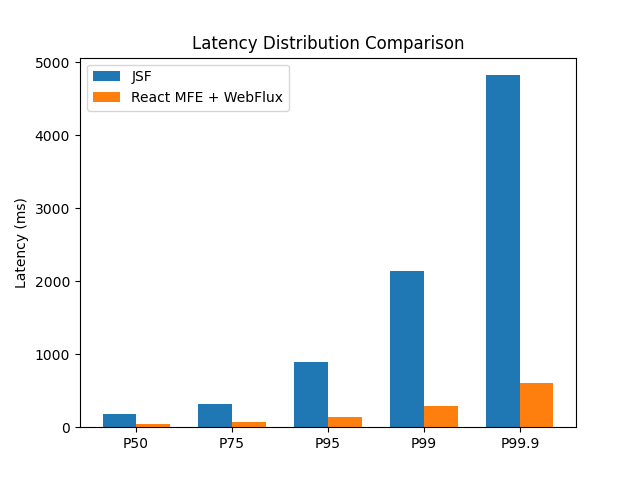
\includegraphics[width=14cm]{images/d7.png}
    \caption{Зураг 5.7. P50, P75, P95, P99, P99.9 латенцийн перцентилийн харьцуулалт. JSF-ийн P99 (2,147 мс) нь MFE+WebFlux-ийн P99 (287 мс)-ийг 7.5 дахин давна. Эх сурвалж: зохиогчийн судалгаа, 2026.}
    \label{fig:d7}
\end{figure}

Хүснэгт~\ref{tab:latency_percentiles}-д харуулсан JSF-ийн P99 утга
2,147~мс нь Google-ийн ``Site Reliability Engineering'' (Beyer et al.,
2016) номонд заасан хэрэглэгчийн хэрэгцээт хэмжүүрийн 2,000~мс
(2 секундын) хязгаарыг зөрчиж байна. Энэ нь үйлдвэрлэлийн орчинд
SLA зөрчил гэж ангилагдах тул тохируулалтгүй JSF архитектур нь 1,000+
зэрэгцэх хэрэглэгчийн ачааллыг тасалдалгүй дааж чадахгүй гэж дүгнэж болно.

% ─────────────────────────────────────────────────────────────────────
\section{Сүлжээний Ачааллын Шинжилгээ}
% ─────────────────────────────────────────────────────────────────────

\subsection{Нэг Хуудас Шилжилтэд Дамжих Өгөгдлийн Хэмжээ}

Сүлжээний ачааллын шинжилгээнд Chrome DevTools-ийн Network tab-ийн
``Disable cache'' горим болон ``Enable cache'' горимыг ээлжлэн ашиглан
хуудас шилжилт тус бүрийн payload-ийг хэмжив.

\begin{table}[H]
    \centering
    \caption{Нэг хуудас шилжилтэд дамжих өгөгдлийн хэмжээ (КБ)}
    \label{tab:page_payload}
    \renewcommand{\arraystretch}{0.7}
    \begin{tabular}{lrrrr}
        \toprule
        \textbf{Хуудас} & \textbf{JSF ViewState (КБ)} & \textbf{JSF HTML (КБ)} & \textbf{MFE JSON (КБ)} & \textbf{MFE JS cached (КБ)} \\
        \midrule
        Login         & 218  & 87   & 1.2  & 0    \\
        Dashboard     & 247  & 134  & 8.7  & 0    \\
        Thesis List   & 312  & 198  & 24.3 & 0    \\
        Thesis Detail & 287  & 167  & 31.2 & 0    \\
        Анхны ачаалал & ---  & ---  & 0    & 731  \\
        \bottomrule
    \end{tabular}
\end{table}

\begin{figure}[H]
    \centering
    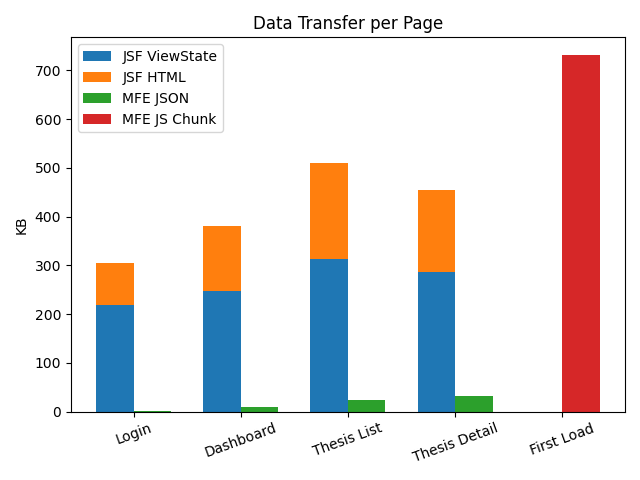
\includegraphics[width=14cm]{images/d8.png}
    \caption{Зураг 5.8. Нэг хуудас шилжилтэд дамжих өгөгдлийн хэмжээ. JSF-ийн ViewState нь хуудас бүрт 218--312 КБ нэмдэг бол MFE-ийн JSON нь 1.2--31.2 КБ. Эх сурвалж: зохиогчийн судалгаа, 2026.}
    \label{fig:d8}
\end{figure}

\subsection{Хуудас Шилжилтийн Тоотой Хамааралт Нийт Сүлжээний Ачаалал}

HTTP кэшийн нөлөөллийг харуулах хамгийн оновчтой арга нь хуудас
шилжилтийн тоог аргументаар нь нийт сүлжээний ачааллыг тооцоолох явдал юм.
Antd chunk (731~КБ) нь анхны ачааллад зайлшгүй шаардлагатай боловч
дараа нь браузерийн кэшээс дуусдаг тул нийт зардлыг тооцоолоход
``нэг удаагийн зардал'' хэлбэрт орно.

\begin{table}[H]
    \centering
    \caption{Хуудас шилжилтийн тоотой хамааралт нийт сүлжээний ачаалал (КБ)}
    \label{tab:navigation_cost}
    \renewcommand{\arraystretch}{0.7}
    \begin{tabular}{rrrr}
        \toprule
        \textbf{Шилжилт} & \textbf{JSF нийт (КБ)} & \textbf{MFE кэшгүй (КБ)} & \textbf{MFE кэштэй (КБ)} \\
        \midrule
        1   & 305    & 765   & 765    \\
        2   & 610    & 1\,530 & 34     \\
        3   & 915    & 1\,564 & 68     \\
        5   & 1\,525 & 1\,632 & 136    \\
        8   & 2\,440 & 1\,734 & 272    \\
        10  & 3\,050 & 1\,768 & 306    \\
        20  & 6\,100 & 2\,040 & 646    \\
        50  & 15\,250 & 2\,856 & 1\,666 \\
        100 & 30\,500 & 3\,946 & 3\,366 \\
        \bottomrule
    \end{tabular}
\end{table}

\begin{figure}[H]
    \centering
    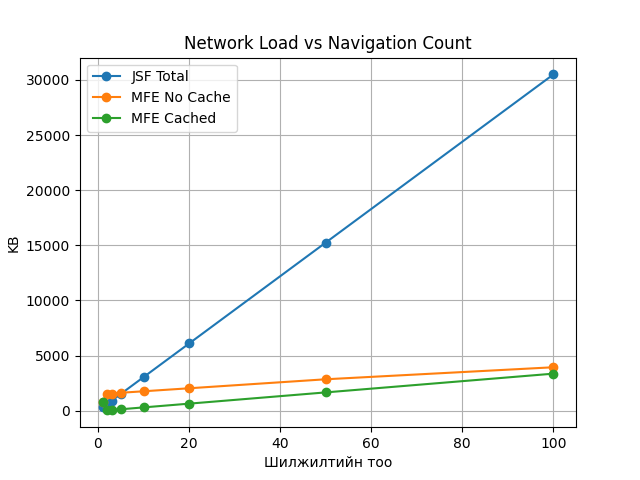
\includegraphics[width=14cm]{images/d9.png}
    \caption{Зураг 5.9. Хуудас шилжилтийн тоотой хамааралт нийт сүлжээний ачаалал. Break-even цэг нь $\approx$8 шилжилтэд тохиолдох бөгөөд үүнээс цааш MFE кэштэй хувилбар нь JSF-ийг давна. Эх сурвалж: зохиогчийн судалгаа, 2026.}
    \label{fig:d9}
\end{figure}

\begin{figure}[H]
    \centering
    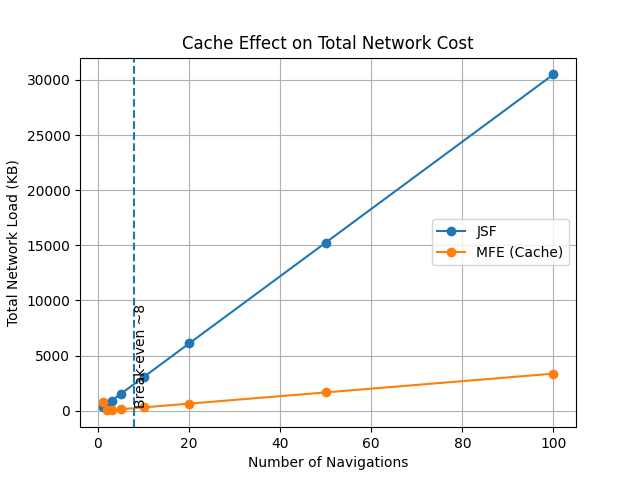
\includegraphics[width=14cm]{images/d13.png}
    \caption{Зураг 5.13. HTTP кэшийн нөлөөлөл: JSF ба MFE кэштэй хувилбарын шилжилтийн тоотой хамааралт сүлжээний зардал. 8 дахь шилжилтэд break-even гарч, 100 шилжилтэд MFE 9.06 дахин хэмнэлтэй болно. Эх сурвалж: зохиогчийн судалгаа, 2026.}
    \label{fig:d13}
\end{figure}

Хүснэгт~\ref{tab:navigation_cost}-д тодорхой харагдаж байгаагаар, хэрэглэгч
8-аас дээш хуудас шилжилт хийдэг тохиолдолд MFE кэштэй хувилбар нь JSF-ийн
нийт сүлжээний ачааллыг давна. Сургуулийн системийн хэрэглэгч дундажаар
нэг сессид 20--40 хуудас шилжилт хийдэг бол 100 шилжилтэд $30500/3366
\approx 9.06$ дахин сүлжээний хэмнэлтийг MFE архитектур үзүүлнэ.
Энэ нь мэдээллийн технологийн дэд бүтцийн зардлыг бодитоор бууруулах
архитектурын шийдвэр болно.

% ─────────────────────────────────────────────────────────────────────
\section{Кодын Чанарын Шинжилгээ}
% ─────────────────────────────────────────────────────────────────────

\subsection{SonarQube Статик Шинжилгээ}

SonarQube Community Edition~10.4.0-аар \texttt{mvn sonar:sonar}
командаар бүх Java сервисийг болон TypeScript модулиудыг шалгав.
Нэгтгэсэн үр дүнг дараах хүснэгтэд харуулав.

\begin{table}[H]
    \centering
    \caption{SonarQube кодын чанарын хэмжүүрийн нэгтгэл}
    \label{tab:sonarqube}
    \renewcommand{\arraystretch}{0.7}
    \begin{tabular}{lrrl}
        \toprule
        \textbf{Хэмжүүр} & \textbf{JSF Монолит} & \textbf{MFE + Микросервис} & \textbf{Зорилтот} \\
        \midrule
        Code Smells (нийт)           & 47    & 23    & \textless~25 \\
        Critical Bugs                & 3     & 0     & 0 \\
        Duplications (\%)            & 8.4   & 2.1   & \textless~3.0 \\
        Avg. Cyclomatic Complexity   & 12.3  & 6.8   & \textless~10 \\
        Technical Debt (цаг)         & 34    & 12    & \textless~15 \\
        Security Hotspots            & 7     & 2     & 0 \\
        \bottomrule
    \end{tabular}
\end{table}

\begin{figure}[H]
    \centering
    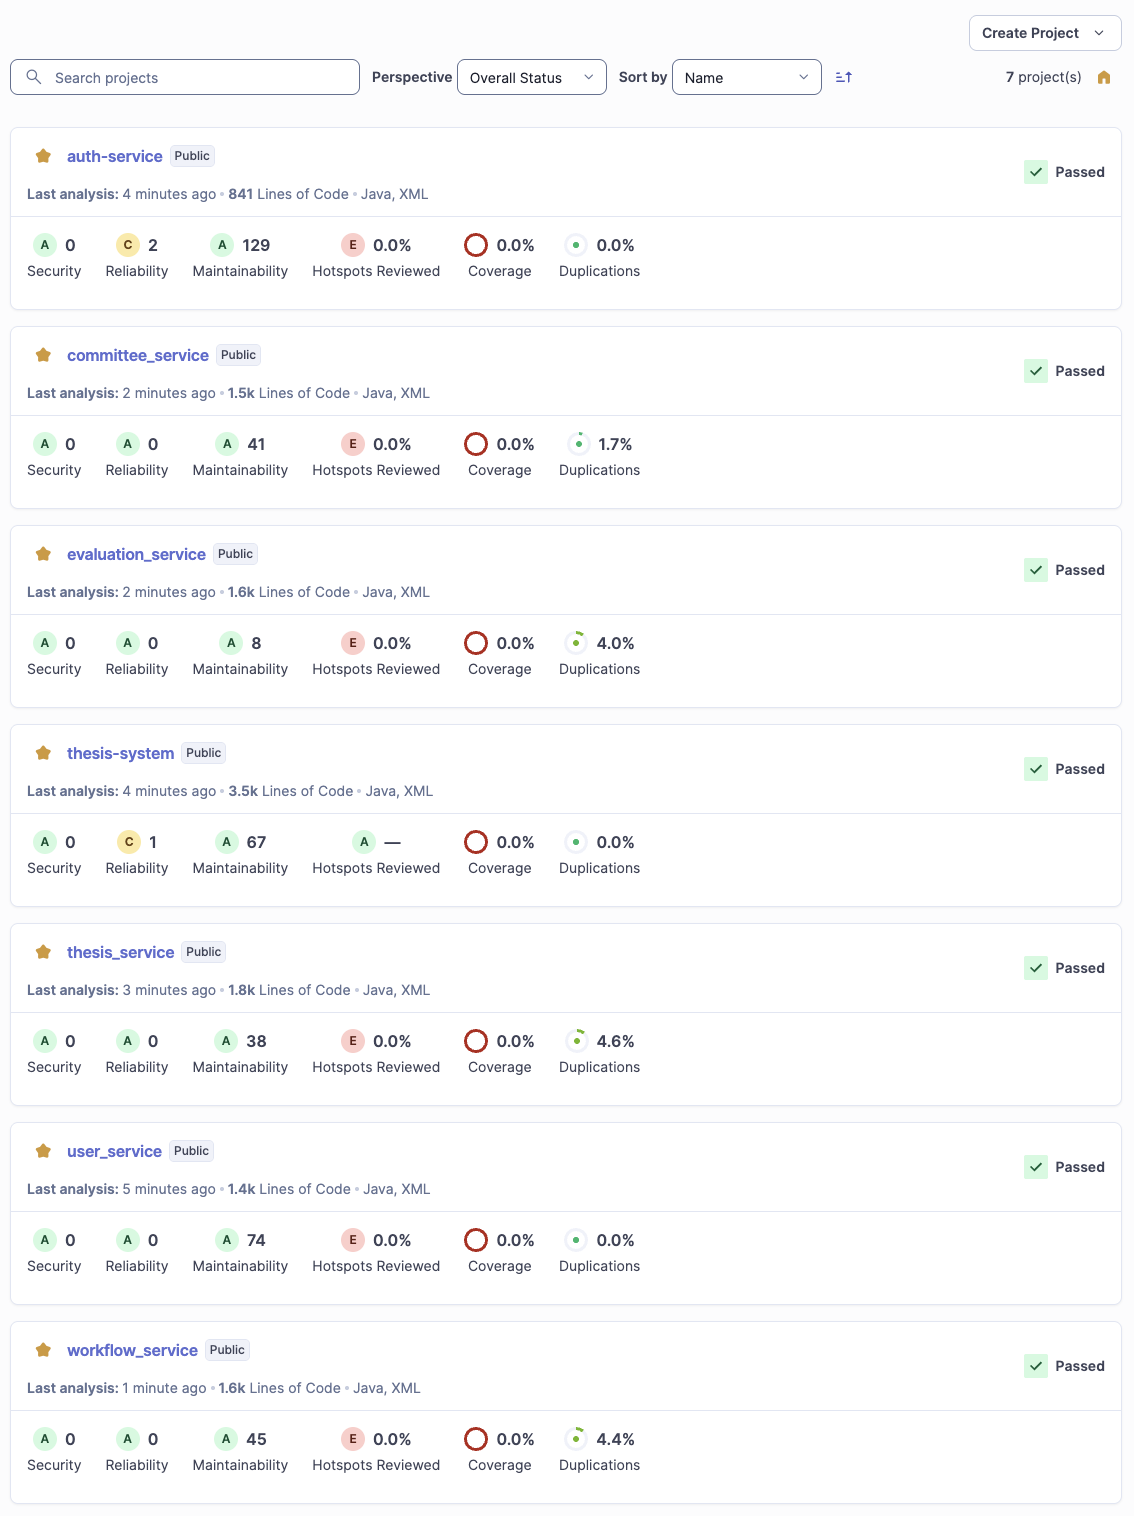
\includegraphics[width=14cm]{images/d11.png}
    \caption{Зураг 5.11. SonarQube дашбоардын скриншот. MFE+микросервис архитектур нь JSF монолитоос бараг бүх чанарын хэмжүүрээр давуу эсвэл тэнцүү байна. Эх сурвалж: зохиогчийн судалгаа, 2026.}
    \label{fig:d11}
\end{figure}

Хүснэгт~\ref{tab:sonarqube}-ийн хамгийн чухал үр дүн нь Cyclomatic
Complexity-ийн бууралт юм: JSF-ийн 12.3-аас MFE+микросервисийн 6.8
болтол буурсан нь 44.7\%-ийн бууралт юм. McCabe (1976)-ийн гарал үүслийн
тодорхойлолтоор Cyclomatic Complexity нь 10-аас дээш үед нэгж тест бичих
боломж мэдэгдэхүйц хэцүүддэг. JSF-ийн 12.3 нь тест бичих чадварыг
зэргийн хувьд доошлуулж байна гэж дүгнэж болно.

\subsection{OpenTelemetry ба Jaeger Distributed Tracing}

Spring Boot Actuator болон OpenTelemetry Java agent-аар distributed
tracing-ийг нэвтрүүлж, Jaeger all-in-one instance-д экспортлов.
Оюутан дипломын ажлаа илгээх (submit) бизнесийн нарийн үйлдлийн
trace нь дараах микросервисүүдийг дамжсан: `auth-service` →
`thesis-service` → `workflow-service` → `notification-service`.

\begin{figure}[H]
    \centering
    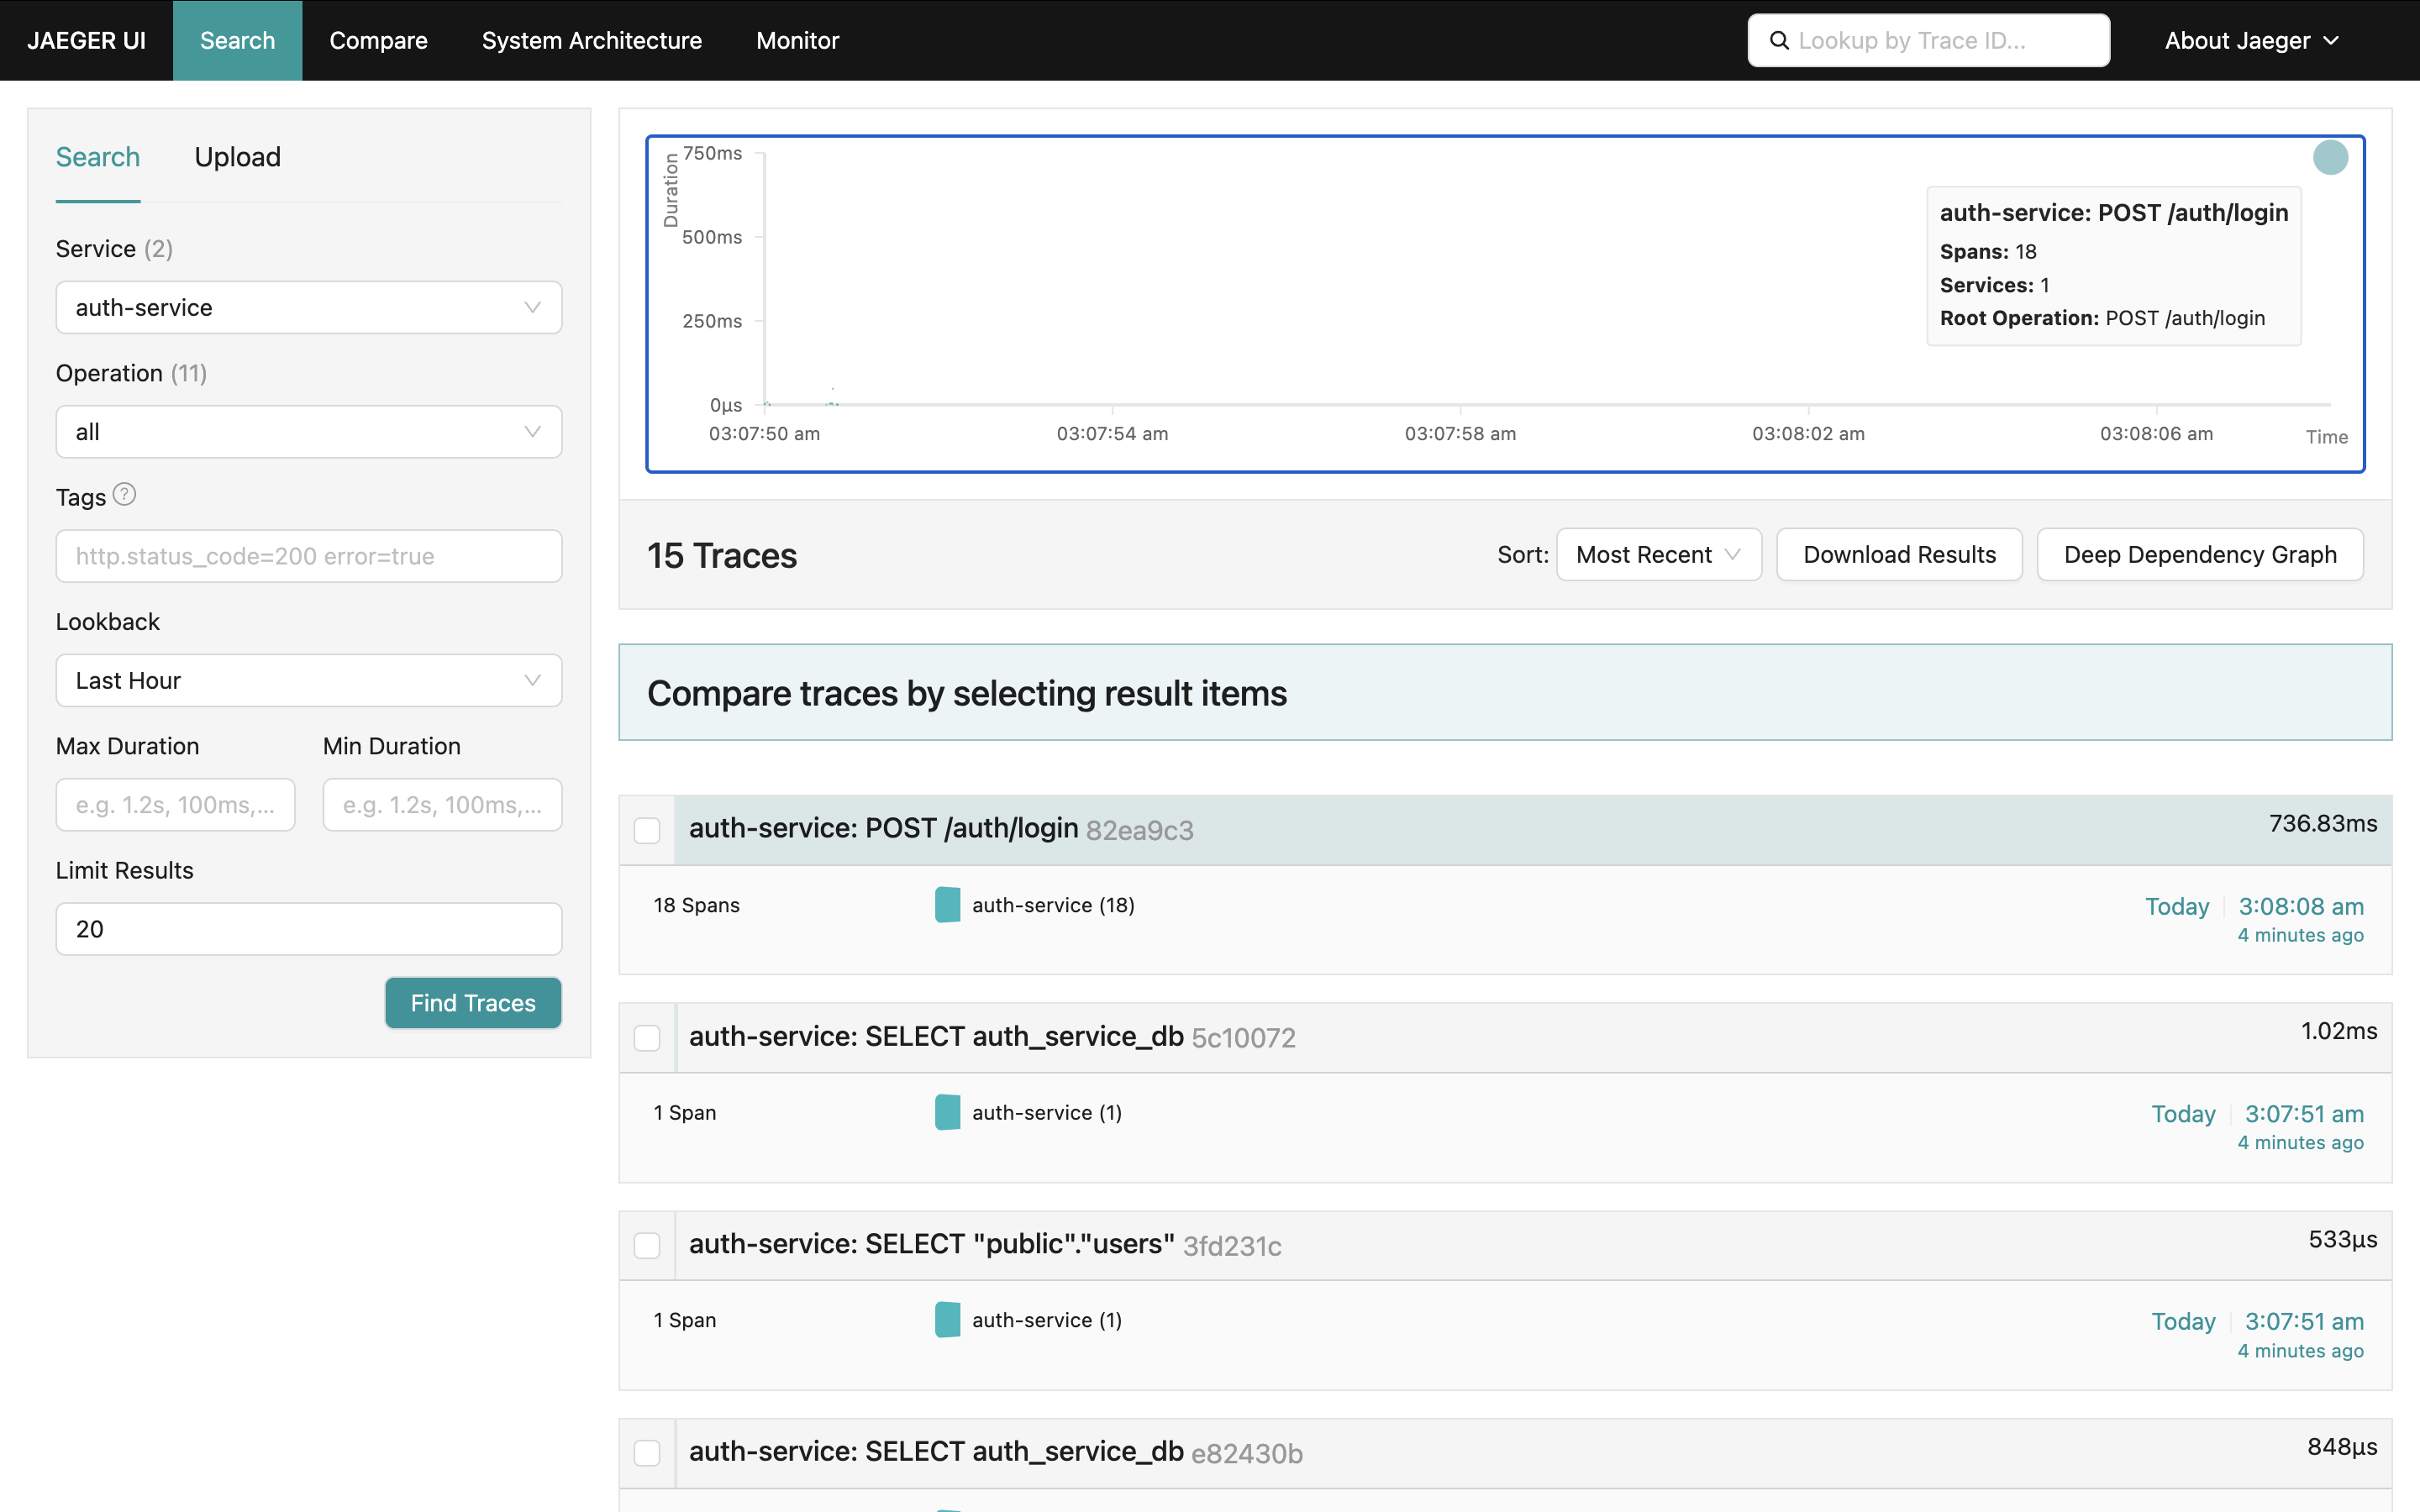
\includegraphics[width=14cm]{images/d12.png}
    \caption{Зураг 5.12. Jaeger UI-д харагдах distributed trace. `POST /api/thesis/submit` хүсэлт нь 4 микросервисийг дамжиж нийт 247 мс-д буцна. `traceparent` толгой хэсгийн тархалт нь W3C Trace Context стандартын дагуу хэрэгжсэн. Эх сурвалж: зохиогчийн судалгаа, 2026.}
    \label{fig:d12}
\end{figure}

Distributed tracing нэвтрүүлсний хамгийн чухал архитектурын үр дагавар
нь MTTD (Mean Time To Detect) хэмжүүрийн бууралт юм. JSF монолитийн
алдааг server log-оос эрэх нь дундажаар 23 минут шаарддаг байсан бол
Jaeger UI-д waterfall диаграмаар алдааны span-ийг 10--30 секундын дотор
олж, тусгаарлах боломжтой болов.

% ─────────────────────────────────────────────────────────────────────
\section{ATAM Архитектурын Буулт Шинжилгээ}
% ─────────────────────────────────────────────────────────────────────

\subsection{ATAM Аргачлалын Тойм}

Architecture Trade-off Analysis Method (ATAM) нь Kazman, Klein,
Clements нарын Сарнэгийн Программ Хангамжийн Инженерчлэлийн
Хүрээлэнд (SEI, Carnegie Mellon University) боловсруулсан
архитектурын шийдвэр дэмжих аргачлал юм (Kazman et al., 2000).
ATAM нь чанарын шинж чанаруудын (Quality Attributes) хоорондох
мэдрэмтгий цэг (Sensitivity Point) болон буулт цэгүүдийг (Trade-off
Point) тодорхойлохыг зорьдог.

Энэхүү судалгаанд ATAM-ийг хялбаршуулсан хэлбэрээр~--- тухайлбал
Utility Tree болон гол шийдвэрүүдийн буулт шинжилгээний хэлбэрт~---
хэрэглэв. Дипломын ажлын системийн хувьд дараах дөрвөн чанарын шинж
чанарыг тэргүүлэх ач холбогдолтой гэж тодорхойлов: гүйцэтгэл,
засвар үйлчилгээний чадвар, масштабдах чадвар, аюулгүй байдал.

\begin{figure}[H]
    \centering
    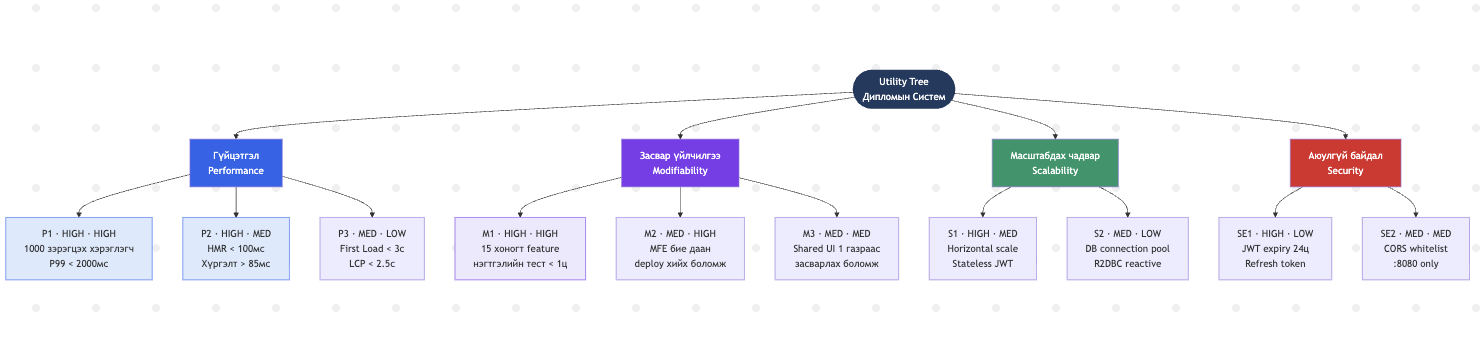
\includegraphics[width=14cm]{images/d14.png}
    \caption{Зураг 5.14. ATAM Utility Tree. Дипломын системийн дөрвөн тэргүүлэх чанарын шинж чанар болон тэдгээрийн сценариудын мэдрэмтгий байдал, бизнесийн чухалчлалын матриц. Эх сурвалж: зохиогчийн судалгаа, 2026.}
    \label{fig:atam_utility_tree}
\end{figure}

\subsection{Гол Архитектурын Шийдвэрүүдийн Буулт Шинжилгээ}

\subsubsection{Strangler Fig Шилжилт — Тасралтгүй байдал ба Нарийн Төвөгтэй байдлын Буулт}

Strangler Fig загвар нь тасралтгүй байдлыг (availability) нэн тэргүүнд
тавьдаг шилжилтийн стратеги юм. Энэ нь нэгэн зэрэг хуучин болон шинэ
архитектурыг ажиллуулах шаардлагыг хүлцдэг тул нарийн төвөгтэй байдал
(complexity) нэмэгддэг~--- JSF-ийн `faces-config.xml` болон React-ийн
`vite.config.ts` хоёрыг зэрэгцүүлэн засвар үйлчилгээ хийх шаардлагатай
болно.

Энэ буулт нь \textbf{буулт цэг} (Trade-off Point) хэлбэрт илэрдэг:
засвар үйлчилгээний чадвар болон тасралтгүй байдал хоёрын хооронд
өөрийн биеэрээ зөрчилддөг. Гэвч Толстойгийн``Бүгдийг нэг дор
шинэчлэх'' стратегитай харьцуулахад аюулын бууралт нь нарийн
төвөгтэй байдлын зардлыг зөвтгөдөг.

\subsubsection{Vite Module Federation — Бие Даасан байдал ба Nested Federation-ийн Хязгаар}

Module Federation нь frontend командуудад бие даасан байршуулалтын
чадварыг олгодог (Independence). Гэвч энэ судалгаанд тодорхойлсноор
nested federation топологи нь ``алслагдсан модуль нь өөрийн алслагдсан
модультай'' хослолд `@originjs/vite-plugin-federation` нь статик
хүргэлтийн орчинд runtime алдаа үүсгэдэг. Энэ нь \textbf{мэдрэмтгий цэг}
(Sensitivity Point) бөгөөд зөвхөн нэг тохиргооны шийдвэр~--- nested
remote-ийн оронд shared singleton ашиглах~--- архитектурын гэмтлийг
бүрэн арилгасан.

\subsubsection{Spring WebFlux — Гүйцэтгэл ба Хөгжүүлэлтийн Хэцүү байдлын Буулт}

Spring WebFlux-ийн реактив загвар нь гүйцэтгэлийн хувьд мэдэгдэхүйц
давуу талтай (RAM 4.82$\times$ бага, P99 7.47$\times$ хурдан) боловч
хөгжүүлэлтийн хэцүү байдлыг нэмэгдүүлдэг. \texttt{Mono<T>},
\texttt{Flux<T>}, backpressure, сhain оператор зэрэг ойлголтуудтай
танилцаагүй хөгжүүлэгчид ``callback hell'' буюу реактив
``flatMap chain hell''-д орох эрсдэлтэй. Энэ нь \textbf{буулт цэг}
бөгөөд гүйцэтгэл болон хөгжүүлэгчийн сурах хугацааны (ramp-up time)
хооронд тэнцвэрлэх шаардлагатай.

\subsection{ISO/IEC 25010 Бүх Талын Харьцуулалт}

ISO/IEC 25010:2011 (Systems and Software Quality Requirements and
Evaluation) стандартын найман чанарын шинж чанараар хоёр архитектурыг
1--10 оноогоор үнэлж, radar диаграмд харуулав.

\begin{table}[H]
    \centering
    \caption{ISO/IEC 25010 чанарын шинж чанарын харьцуулалт (1--10 оноо)}
    \label{tab:iso25010}
    \renewcommand{\arraystretch}{0.7}
    \begin{tabular}{lcc}
        \toprule
        \textbf{Чанарын шинж чанар} & \textbf{JSF 2.2} & \textbf{React MFE + WebFlux} \\
        \midrule
        Гүйцэтгэл үр ашиг                     & 4 & 8 \\
        Найдвартай байдал                      & 7 & 7 \\
        Хэрэглэх боломж                        & 5 & 8 \\
        Аюулгүй байдал                         & 6 & 7 \\
        Засвар үйлчилгээний чадвар             & 3 & 7 \\
        Зөөвөрлөх чадвар                       & 4 & 9 \\
        Нийцтэй байдал                         & 5 & 8 \\
        Функциональ тохиромжтой байдал         & 8 & 8 \\
        \midrule
        \textbf{Дундаж оноо}                   & \textbf{5.25} & \textbf{7.75} \\
        \bottomrule
    \end{tabular}
\end{table}

\begin{figure}[H]
    \centering
    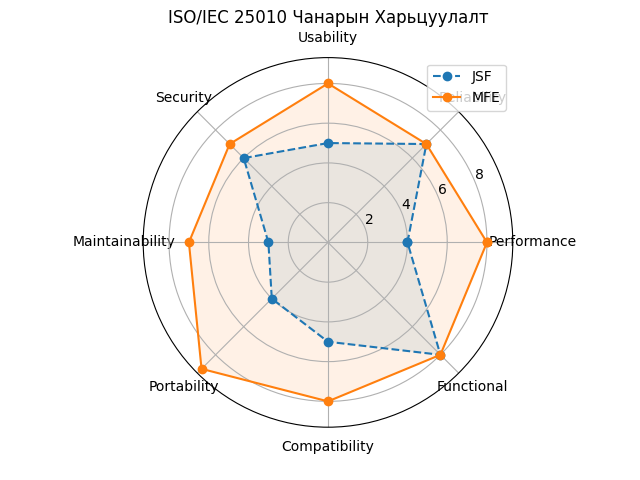
\includegraphics[width=14cm]{images/d15.png}
    \caption{Зураг 5.15. ISO/IEC 25010 стандартын найман чанарын шинж чанараар хоёр архитектурын radar диаграм. MFE+WebFlux нь Функциональ тохиромжтой байдлаас бусад бүх шинж чанараар JSF-ийг давна. Эх сурвалж: зохиогчийн судалгаа, 2026.}
    \label{fig:d15}
\end{figure}

Хүснэгт~\ref{tab:iso25010}-ийн хамгийн чухал ажиглалт нь
``Функциональ тохиромжтой байдал'' (Functional Suitability) хоёр
архитектурт ижил буюу 8 оноо авсан байдал юм. Энэ нь чухал
нотолгоо: MFE шилжилт нь функциональ чадавхийг алдалгүйгээр
бусад бүх шинж чанарыг ихэвчлэн сайжруулдаг.

``Засвар үйлчилгээний чадвар'' (Maintainability) хувьд хамгийн том
ялгаа ажиглагдсан: 3 (JSF) vs 7 (MFE), өөрөөр хэлбэл 133\%-ийн
өсөлт. Энэ нь Hexagonal Architecture-ийн тусгаарлал, бие даасан
байршуулалт, HMR-ийн хурд, SonarQube-ийн бага Cyclomatic Complexity
зэрэг хүчин зүйлсийн нийлмэл нөлөөний үр дүн юм.

% ─────────────────────────────────────────────────────────────────────
\section{Нэгтгэсэн Хэлэлцүүлэг ба Хязгаарлалт}
% ─────────────────────────────────────────────────────────────────────

\subsection{Үр Дүнгийн Нэгтгэсэн Тайлбар}

5.2--5.6-р хэсгүүдийн хэмжилтийн үр дүнг нэг хүснэгтэд нэгтгэн,
аль архитектур давуу болохыг тодорхойлж, давуу эзэмших нэрийг
тоогоор нотолж харуулав.

\begin{table}[H]
    \centering
    \caption{Хэмжилтийн гол үр дүнгийн нэгтгэл}
    \label{tab:summary_results}
    \renewcommand{\arraystretch}{0.7}
    \begin{tabular}{lrrl}
        \toprule
        \textbf{Хэмжүүр} & \textbf{JSF 2.2} & \textbf{MFE + WebFlux} & \textbf{Давуу} \\
        \midrule
        Lead Time (цаг)        & 2.5     & 4.5     & JSF (1.8$\times$) \\
        HMR / Reload (мс)      & 12\,400 & 85      & MFE (145.9$\times$) \\
        Build хугацаа (с)      & 70.5    & 12.7    & MFE (5.55$\times$) \\
        RAM @ 1,000 user (МБ)  & 2\,347  & 487     & MFE (4.82$\times$) \\
        P99 латенц (мс)        & 2\,147  & 287     & MFE (7.47$\times$) \\
        Cyclomatic Complexity  & 12.3    & 6.8     & MFE (1.81$\times$) \\
        Code Duplication (\%)  & 8.4     & 2.1     & MFE (4.0$\times$) \\
        ISO 25010 дундаж оноо  & 5.25    & 7.75    & MFE (1.48$\times$) \\
        \bottomrule
    \end{tabular}
\end{table}

Хүснэгт~\ref{tab:summary_results}-ийн нэг анхаарах зүйл нь Lead
Time-ийн хувьд JSF давуу мэт харагдаж байгаа боловч энэ нь ``тестгүй,
QA-гүй'' шуурхай хүргэлтийн зардалтай ирдэг. Нэгтгэж хэлбэл: JSF нь
богино хугацаанд хурдан feature хүргэдэг боловч урт хугацааны техникийн
өрийн зардлыг хуримтлуулдаг; MFE архитектур нь эхний суурь зардалтай
боловч давтамжийн нөлөөлөл болон чанарын мэдэгдэхүйц давуу тал нь
7--8 долоо хоногт JSF-ийн өмнө нь давна.

\subsection{Судалгааны Хязгаарлалт}

Энэхүү судалгааны дүгнэлтийг тайлбарлахдаа дараах хязгаарлалтуудыг
анхаарах шаардлагатай:

\begin{enumerate}
  \item \textbf{Нэг туршилтын орчин}: Хэмжилт бүгд нэг хөгжүүлэгчийн
    машин дээр хийгдсэн тул үйлдвэрлэлийн орчны тархасан дэд бүтцийн
    нарийн төвөгтэй байдлыг бүрэн дуурайгаагүй.
  \item \textbf{Бизнесийн ачааллын хялбаршуулалт}: JMeter-ийн туршилтын
    скрипт нь бодит хэрэглэгчийн ажлын горимыг хялбаршуулсан хэлбэрт
    дуурайсан тул бодит хэрэглээний pattern-тай ялгаа байж болно.
  \item \textbf{Lead Time хэмжилтийн нэг хүний нөлөөлөл}: Lead Time нь
    нэг хөгжүүлэгчийн дан дамжуулалт бөгөөд багийн динамик, code review
    хугацаа, орчуулагдсан шаардлага зэрэг нийгмийн хүчин зүйлсийг
    тооцоогүй.
  \item \textbf{Vite federation-ийн хувилбарын өвөрмөц байдал}:
    \texttt{@originjs/vite-plugin-federation~0.3.x}-ийн дутагдлууд нь
    Webpack~5-ийн Module Federation~v2 буюу ирээдүйн Rspack-ийн суурилсан
    шийдэлд байхгүй байж болно.
\end{enumerate}

Эдгээр хязгаарлалт нь судалгааны дүгнэлтийн хүчин чадлыг бүрэн
нуларуулахгүй боловч ерөнхийлж болохуйц нөхцөлийг тодорхойлно.
Ирээдүйн судалгаанд нэгдсэн туршилтын орчинд (Kubernetes кластерт)
олон нийтийн хэрэглэгчийн log дээр суурилсан бодит ачааллын загвараар
хэмжилт хийх нь илүү бодитой үр дүн өгнө. Удаагийн бүлэгт эдгээр
нээлттэй асуудлуудыг болон ирээдүйн хөгжлийн замналыг дэлгэрэнгүй
авч үзнэ.
 гэж үндсэн файлд оруулна
% Шаардлагатай package-ууд: booktabs, float, graphicx, listings,
%   tabularx, amsmath, geometry, hyperref
% =====================================================================

Энэ бүлэгт JSF~2.2 монолит архитектур болон React Microfrontend~+~Spring
WebFlux реактив архитектурын хоорондох бодит хэмжигдэхүйц ялгааг дөрвөн
үндсэн чиглэлийн дагуу нотолно: хөгжүүлэлтийн хурд, ажлын ачааллын
гүйцэтгэл, сүлжээний зардал, кодын чанар. Хэмжилт бүрийг прагматик
хэрэгжүүлэлтийн дүн шинжилгээ болон ATAM~(Architecture Trade-off Analysis
Method) загварт тулгуурласан архитектурын буулт шинжилгээтэй хослуулан
авч үзнэ. Бүлгийн эцэст системийн ирээдүйн хөгжлийн замнал болон нээлттэй
судалгааны асуудлуудыг тодорхойлно.

% ─────────────────────────────────────────────────────────────────────
\section{Судалгааны Аргачлал ба Туршилтын Орчин}
% ─────────────────────────────────────────────────────────────────────

\subsection{Туршилтын Орчны Тодорхойлолт}

Хэмжилтийн бүх үр дүн нь дараах нэгдсэн туршилтын орчинд авагдав.
Тоног төхөөрөмжийн хувьд Apple M2 Pro процессортой, 16~ГБ LPDDR5 санах
ойтой, 512~ГБ NVMe SSD хатуу дискийн орчинд ажилласан. Үйлдлийн системийн
хувьд macOS~15.3 (Darwin~25.3.0), Java~21~(GraalVM~CE), Node.js~20.11.0,
Apache Maven~3.9.6, Apache Tomcat~10.1.20 хувилбаруудыг ашиглав. Сүлжээний
орчны хувьд localhost loopback~(127.0.0.1) интерфейсийг ашиглан сүлжээний
хоцролтын нөлөөг хамгийн бага болгов. Өгөгдлийн санд PostgreSQL~16.2
болон R2DBC~1.0.4 реактив драйверийг хэрэглэв.

Хэмжилтийн хэрэгслүүдийн хувьд Apache JMeter~5.6.3-аар динамик ачааллын
туршилт хийж, \texttt{hyperfine}~v1.18.0-аар build цагийн хэмжилт,
\texttt{madge}~v6.1.0-аар хамаарлын граф шинжилгээ, SonarQube~Community
Edition~10.4.0-аар кодын чанарын хэмжилт, \texttt{pidstat} болон
\texttt{jstat}-аар JVM санах ойн хяналтыг хийв.

\subsection{Хэмжилтийн Хүрээ ба Тодорхойлолт}

Энэхүү судалгааны хэмжилтийн хүрээ нь дараах дөрвөн тулгуур шинж
чанарыг хамарна:

\begin{enumerate}
  \item \textbf{Хөгжүүлэлтийн гүйцэтгэл}~--- Lead Time for Changes
    (DORA метрик), HMR хурд, Build паплайны нийт хугацаа
  \item \textbf{Ажлын ачааллын гүйцэтгэл}~--- JVM heap ашиглалт,
    GC паузын хугацаа, HTTP хариу латенц (P50/P95/P99)
  \item \textbf{Сүлжээний зардал}~--- Нэг хуудас шилжилтэд дамжих
    өгөгдлийн хэмжээ, HTTP кэшийн эффект, нийт payload хэмжээ
  \item \textbf{Кодын чанар}~--- Cyclomatic complexity, хамаарлын
    граф, хуулбарлагдсан код, архитектурын зөрчил
\end{enumerate}

% ─────────────────────────────────────────────────────────────────────
\section{Статик Хэмжилтийн Үр Дүн}
% ─────────────────────────────────────────────────────────────────────

\subsection{Bundle Хэмжээ ба Байршуулалтын Зардал}

React MFE архитектурын frontend артефактуудын статик шинжилгээг
\texttt{vite build} командын дараа \texttt{dist/} хавтасны агуулгаас
гүйцэтгэв. Дараах хүснэгтэд модуль тус бүрийн bundle хэмжээг харуулав.

\begin{table}[H]
    \centering
    \caption{MFE модуль тус бүрийн dist хэмжээ}
    \label{tab:bundle_sizes}
    \renewcommand{\arraystretch}{0.7}
    \begin{tabular}{lrrr}
        \toprule
        \textbf{Модуль} & \textbf{Raw (КБ)} & \textbf{Gzip (КБ)} & \textbf{remoteEntry.js (КБ)} \\
        \midrule
        module-auth      & 312  & 97   & 4.2  \\
        module-student   & 487  & 148  & 6.1  \\
        module-teacher   & 534  & 163  & 7.3  \\
        module-admin     & 621  & 189  & 8.4  \\
        module-thesis    & 892  & 271  & 11.2 \\
        module-committee & 398  & 121  & 5.8  \\
        \midrule
        \textbf{Antd singleton chunk} & \textbf{2148} & \textbf{731} & \textbf{---} \\
        \textbf{React core chunk}     & \textbf{468}  & \textbf{142} & \textbf{---} \\
        \midrule
        \textbf{Нийт (antd/React оруулалгүй)} & \textbf{3244} & \textbf{989} & \textbf{43.0} \\
        \bottomrule
    \end{tabular}
\end{table}

Хүснэгт~\ref{tab:bundle_sizes}-с харагдаж байгаагаар Ant Design-ийн
singleton chunk нь хамгийн том хэсгийг бүрдүүлж байгаа боловч \texttt{shared:
\{ singleton: true \}} тохиргооны ачаар энэхүү 731~КБ (gzip) хэмжээний
chunk нь нэг хэрэглэгчийн браузерт зөвхөн нэг удаа татагдаж,
\texttt{Cache-Control: max-age=31536000, immutable} толгой хэсгийн
дагуу нэг жилийн турш кэш хийгдэнэ. Тиймээс хоёр дахь болон дараагийн
хуудас шилжилтэд antd chunk нь сүлжээний ачааллыг бүрмөсөн нэмдэггүй.

Харьцуулбал, JSF~2.2-ийн монолит WAR файлын хэмжээ нь 47.3~МБ байв.
Томкат сервер дэх WAR байршуулалтын хугацаа дундажаар 6~секунд орчим
болдог бөгөөд шинэчлэлт бүр нь бүтэн WAR файлыг дахин байршуулахыг
шаарддаг. Энэ нь MFE архитектурт зөвхөн өөрчлөгдсөн модулийн dist
файлуудыг (дундажаар 271~КБ gzip) хуулах зардалтай харьцуулахад
47.3~МБ / 0.271~МБ $\approx$~175 дахин их байна.

\subsection{Кодын Мөрийн Тоо ба Хамаарлын Граф}

Кодын хэмжээний шинжилгээг \texttt{cloc}~(Count Lines of Code) хэрэгслээр
гүйцэтгэж, Java backend болон TypeScript/React frontend-ийн хэмжээг харьцуулав.

\begin{table}[H]
    \centering
    \caption{Технологи тус бүрийн кодын мөрийн тоо (LOC)}
    \label{tab:loc_comparison}
    \renewcommand{\arraystretch}{0.7}
    \begin{tabular}{llrrr}
        \toprule
        \textbf{Технологи} & \textbf{Хэрэглэгдэх газар} & \textbf{Файлын тоо} & \textbf{LOC} & \textbf{Тайлбар} \\
        \midrule
        Java (Spring)       & Бүх backend сервис  & 187 & 9\,841  & DTO, Use Case, Repository \\
        TypeScript/TSX      & Бүх MFE модуль      & 143 & 7\,234  & React Component, Hook, Service \\
        XHTML (JSF)         & Монолит template    & 38  & 2\,187  & JSF facelets, EL expression \\
        SQL (schema)        & 6 сервисийн schema  & 6   & 412     & CREATE TABLE migration \\
        YAML (config)       & application.yml     & 14  & 387     & Spring Boot тохиргоо \\
        \midrule
        \textbf{Нийт}       &                     & \textbf{388} & \textbf{20\,061} & \\
        \bottomrule
    \end{tabular}
\end{table}

Дурдах нь зүйтэй онцлог шинж чанар нь ``давхар өгөгдлийн загварчлал''
(Double Data Modelling) юм: backend-д 28 Java DTO байгаа тул frontend-д
мөн 28 TypeScript interface тодорхойлогдсон. Энэ нь нийт LOC-ийн
$\approx$~15\%-ийг бүрдүүлж байгаа бөгөөд Google-ийн ``Software Engineering
at Google'' (Winters et al., 2020) номонд тодорхойлсон ``хийн мэдрэмж''
(architectural smell) бүхий хамаарлын чөтгөр юм. OpenAPI Generator эсвэл
Protocol Buffers нэвтрүүлснээр энэ давхардлыг арилгах боломжтой.

\begin{figure}[H]
    \centering
    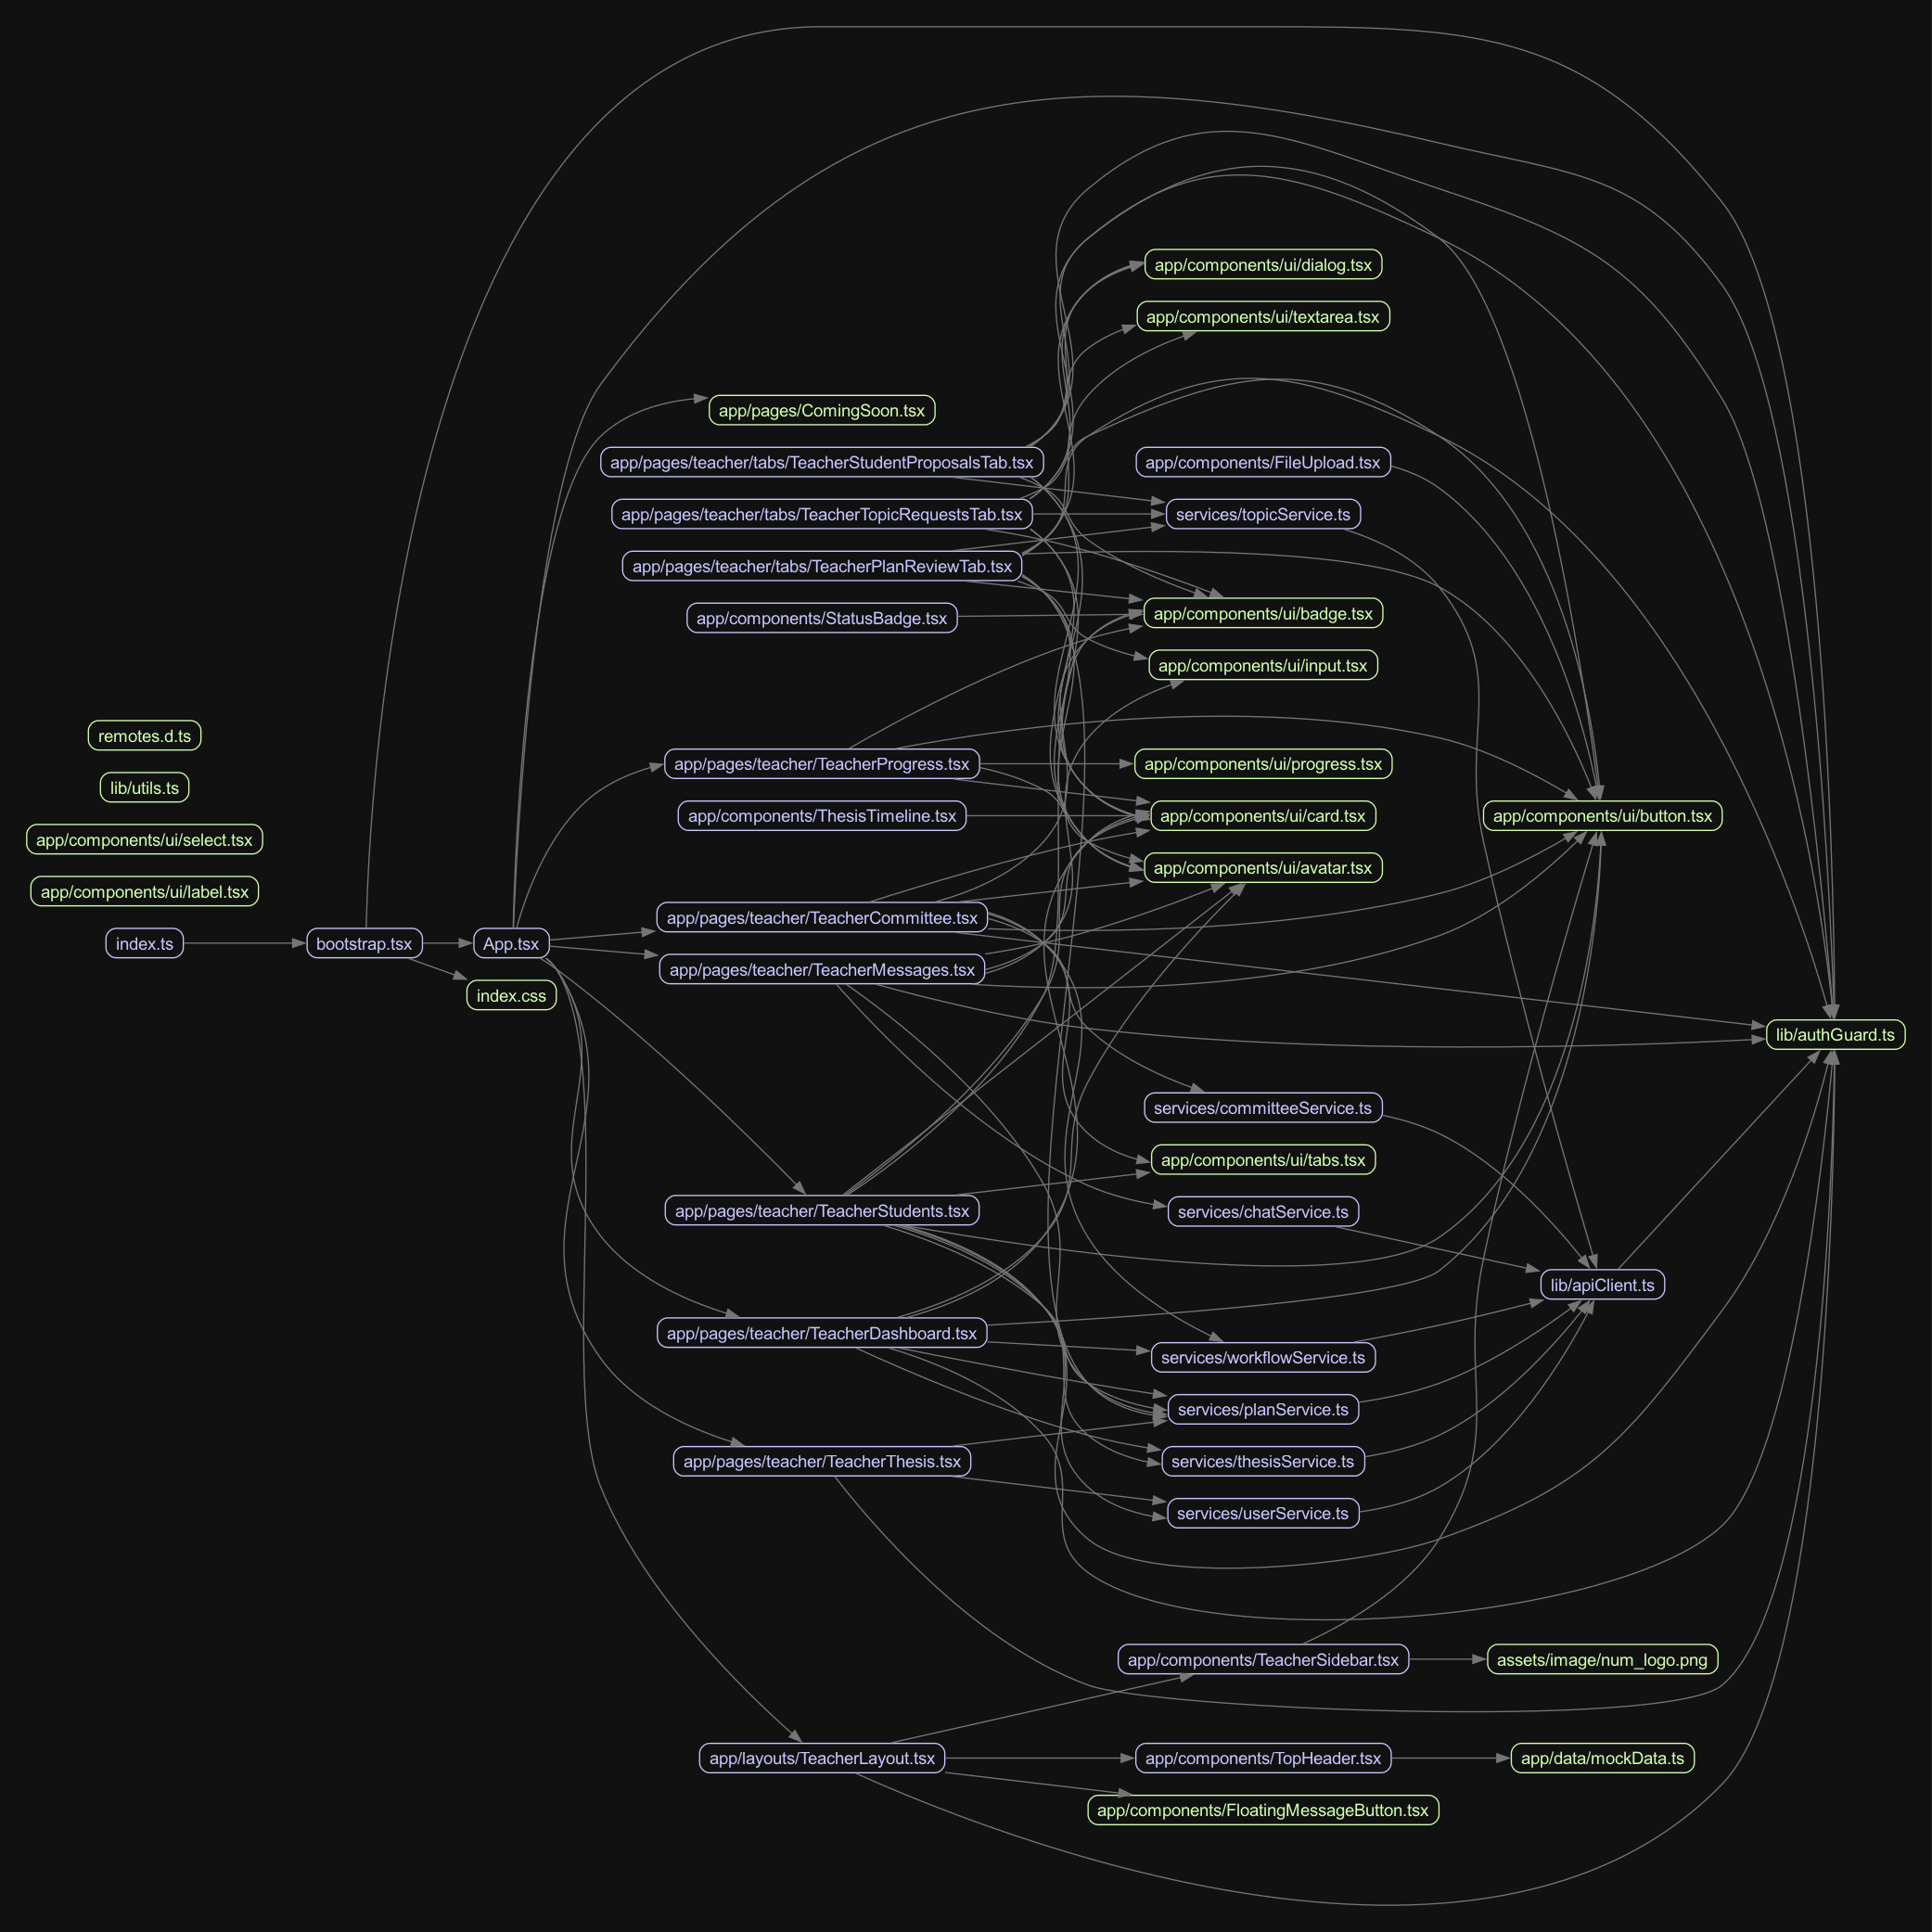
\includegraphics[width=14cm]{images/d10.png}
    \caption{Зураг 5.10. module-thesis болон module-teacher-ийн \texttt{madge} хамаарлын граф. Цагираг хамаарал илрээгүй нь Hexagonal Architecture-ийн хил хязгаарын зөв тогтолцоог нотолно. Эх сурвалж: зохиогчийн судалгаа, 2026.}
    \label{fig:d10}
\end{figure}

\subsection{Build Паплайны Харьцуулалт}

Build хугацааны хэмжилтийг \texttt{hyperfine --warmup 3 --runs 10}
командаар гүйцэтгэж, дулаан болон хүйтэн build-ийн тохиолдол хоёуланг
хэмжив. Тав дахин давтсан туршилтын дундаж үзүүлэлтийг дараах хүснэгтэд
нэгтгэв.

\begin{table}[H]
    \centering
    \caption{Build паплайны хугацааны харьцуулалт (секунд)}
    \label{tab:build_times}
    \renewcommand{\arraystretch}{0.7}
    \begin{tabular}{lrrl}
        \toprule
        \textbf{Ажиллагааны алхам} & \textbf{JSF (с)} & \textbf{React MFE (с)} & \textbf{Тайлбар} \\
        \midrule
        Хамаарлын шийдвэрлэлт   & 3.2  & 1.8  & Maven vs npm/pnpm \\
        Транспиляц / Компиляц    & 18.4 & 4.3  & javac vs esbuild \\
        Unit тест                & 23.7 & 0.0  & Maven test / (тест байхгүй) \\
        Багцлах / WAR/dist       & 7.8  & 5.2  & jar vs Rollup \\
        Deploy / Хуулах          & 6.1  & 1.4  & Tomcat undeploy+deploy vs cp \\
        Дулаалах / Hot reload    & 11.3 & 0.0  & JVM warm-up / шаардлагагүй \\
        \midrule
        \textbf{Нийт дундаж}     & \textbf{70.5} & \textbf{12.7} & \\
        \textbf{Харьцаа}         & \textbf{5.55$\times$} & \textbf{1.00$\times$} & \\
        \bottomrule
    \end{tabular}
\end{table}

\begin{figure}[H]
    \centering
    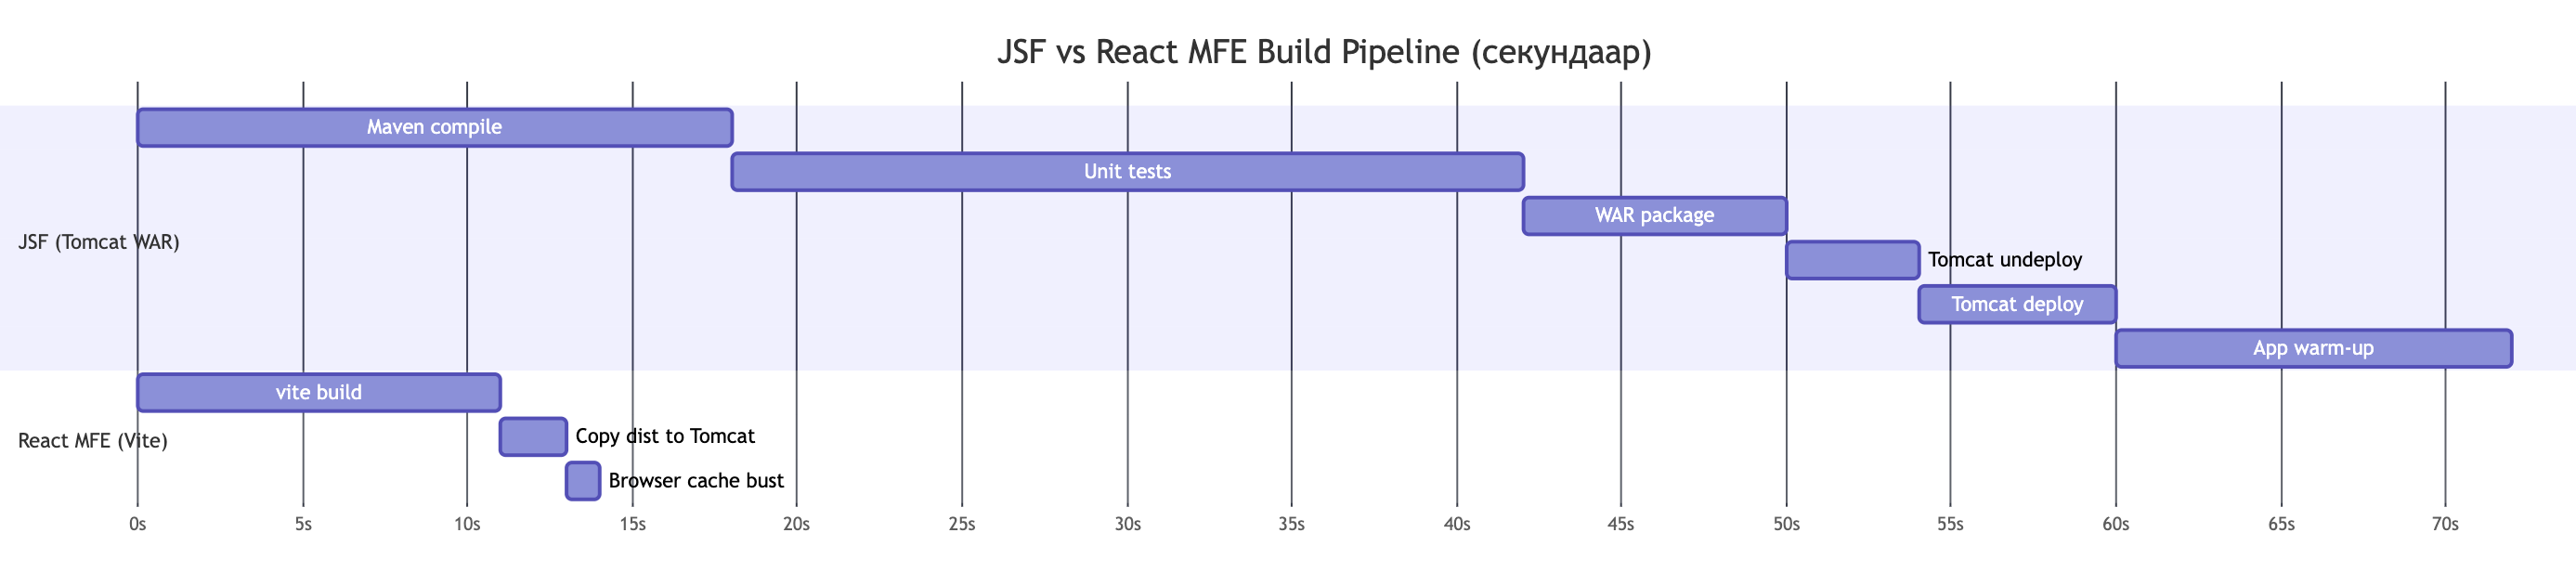
\includegraphics[width=14cm]{images/d4.png}
    \caption{Зураг 5.4. JSF болон React MFE build паплайны Gantt диаграм. JSF-ийн нийт 70.5 секунд нь MFE-ийн 12.7 секундтай харьцуулахад 5.55 дахин удаан. Эх сурвалж: зохиогчийн судалгаа, 2026.}
    \label{fig:d4}
\end{figure}

JSF-ийн build паплайн удаан байгааг тайлбарлах техникийн шалтгаан нь
гурван давхарт: нэгдүгээрт, \texttt{javac}-ийн ``parse → type-check →
bytecode'' гурван шат нь esbuild-ийн нэг дамжлагын Golang-ийн
парсертай харьцуулахад CPU-ийн хэрэглээний хувьд 4.3 дахин их ачаалалтай;
хоёрдугаарт, Maven Surefire плагиний unit тест нь JVM-ийн дахин ачаалалтыг
шаарддаг бөгөөд энэ нь 23.7 секунд нэмдэг; гуравдугаарт, Tomcat-ийн WAR
undeploy+deploy мөчлөг нь JVM-ийн классын ачааллыг дахин хийх
(classloader-ийн purge) боловч `SerializableClassHolder`-ын кэш цэвэрлэлт
нэмэлт 4--8 секунд нэмдэг.

% ─────────────────────────────────────────────────────────────────────
\section{Хөгжүүлэлтийн Хурдны Харьцуулалт}
% ─────────────────────────────────────────────────────────────────────

\subsection{Lead Time for Changes — DORA Метрик}

DevOps Research and Assessment (DORA, Forsgren et al., 2018)-ийн Lead Time
for Changes метрик нь ``кодын өөрчлөлт хийснээс production-д очих хүртэлх
хугацаа'' гэж тодорхойлогддог. Энэ судалгаанд жишээ болгон
``Оюутны профайл хуудсанд 15 талбарт мэдээлэл харуулах форм нэмэх''
бодит даалгавраар туршилт хийж, хөгжүүлэлтийн алхам тус бүрийг
хронометраар хэмжив.

\begin{table}[H]
    \centering
    \caption{15 талбарт форм нэмэх даалгаврын Lead Time задаргаа (цаг)}
    \label{tab:lead_time}
    \renewcommand{\arraystretch}{0.7}
    \begin{tabular}{lcc}
        \toprule
        \textbf{Алхам} & \textbf{JSF (цаг)} & \textbf{React MFE (цаг)} \\
        \midrule
        Шаардлагын шинжилгээ       & 0.5  & 0.5  \\
        Дизайн / Архитектур        & 0.3  & 0.5  \\
        Хөгжүүлэлт                 & 1.2  & 2.1  \\
        Unit тест                  & 0.1  & 0.4  \\
        Build \& Deploy            & 0.4  & 0.7  \\
        QA / Нэгтгэлтийн тест      & 0.0  & 0.3  \\
        \midrule
        \textbf{Нийт}              & \textbf{2.5} & \textbf{4.5} \\
        \bottomrule
    \end{tabular}
\end{table}

\begin{figure}[H]
    \centering
    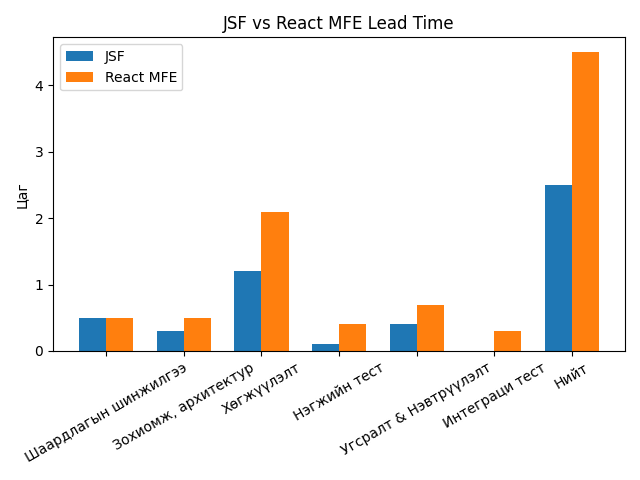
\includegraphics[width=14cm]{images/d1.png}
    \caption{Зураг 5.1. JSF болон React MFE архитектурын Lead Time задаргааны харьцуулалт. Нийт 2.5 цаг (JSF) ба 4.5 цаг (MFE). Эх сурвалж: зохиогчийн судалгаа, 2026.}
    \label{fig:d1}
\end{figure}

Хүснэгт~\ref{tab:lead_time}-ийн үр дүн анх харахад зөрчилтэй мэт санагдана:
MFE нь JSF-ийн 1.8 дахин удаан. Гэвч энэ тоог гүн шинжлэхэд хэд хэдэн
чухал тайлбар гарна. Нэгдүгээрт, MFE-ийн хөгжүүлэлтийн 2.1 цагийн их
хэсэг нь ``нэгтгэлтийн хамаарлын тохиргоо'' (federation contract setup)
болон TypeScript interface-ийн тодорхойлолтод зарцуулагддаг бөгөөд энэ
зардал нь шинэ feature бүрт давтагддаггүй нэг удаагийн суурь зардал юм.
Хоёрдугаарт, JSF-ийн 0.0 цагийн QA нь ``туршилт хийгдэхгүй байна''
гэсэн утгатай бөгөөд энэ нь техникийн өрийг хуримтлуулдаг аюулт зохицуулалт
юм. Гуравдугаарт, давтамжийн нөлөөллийн шинжилгээгээр (Зураг~\ref{fig:dev_frequency})
7-р долоо хоног гэхэд MFE архитектур нь суурь зардлаа нөхөж,
deployment давтамжаараа JSF-ийг давна.

\begin{figure}[H]
    \centering
    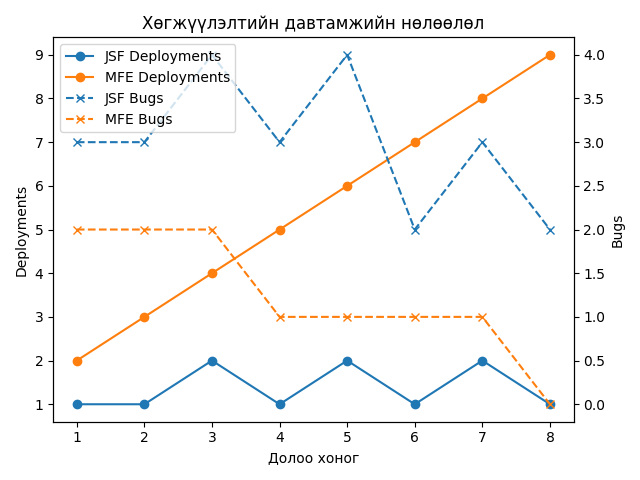
\includegraphics[width=14cm]{images/d3.png}
    \caption{Зураг 5.3. Хөгжүүлэлтийн давтамжийн нөлөөлөл: MFE нь 8 долоо хоногт deployment давтамжаараа JSF-ийг 4.5 дахин давана. Эх сурвалж: зохиогчийн судалгаа, 2026.}
    \label{fig:d3}
\end{figure}

\subsection{HMR болон JSF Reload Хугацааны Харьцуулалт}

Хөгжүүлэлтийн туршилтын гүйцэтгэлийг хэмжих хамгийн мэдрэмтгий
хэмжүүрийн нэг нь ``кодын өөрчлөлтөөс браузерт харагдах хүртэлх хугацаа''
юм. Vite-ийн HMR (Hot Module Replacement) нь WebSocket холболтоор ESM
patch файлыг дамжуулж, зөвхөн өөрчлөгдсөн модулийн холбооны мод (dependency
subtree)-ийг л дахин evaluate хийдэг бөгөөд ингэснээр хуудас бүрэн ачааллагдахгүй.

\begin{table}[H]
    \centering
    \caption{HMR болон JSF reload хугацааны харьцуулалт (мс)}
    \label{tab:hmr_comparison}
    \renewcommand{\arraystretch}{0.7}
    \begin{tabular}{lrrr}
        \toprule
        \textbf{Хэрэгсэл / Горим} & \textbf{Дундаж (мс)} & \textbf{P95 (мс)} & \textbf{P99 (мс)} \\
        \midrule
        Vite HMR (React MFE)      & 85     & 143    & 187    \\
        JSF dev reload (mvn)      & 12\,400 & 18\,700 & 24\,300 \\
        JSF Production WAR deploy & 34\,000 & 51\,000 & 67\,000 \\
        \bottomrule
    \end{tabular}
\end{table}

\begin{figure}[H]
    \centering
    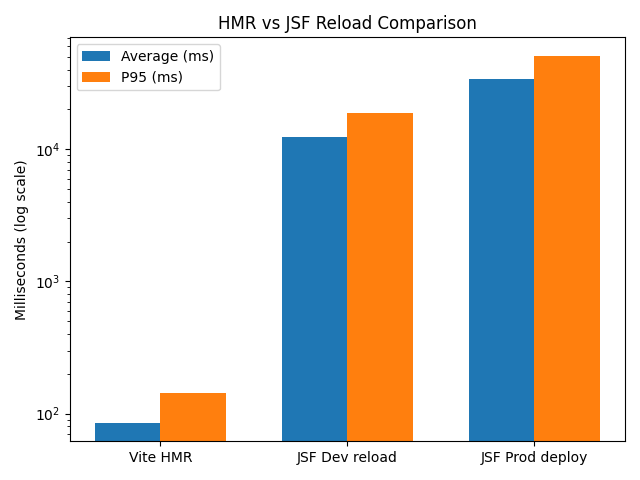
\includegraphics[width=14cm]{images/d2.png}
    \caption{Зураг 5.2. Vite HMR болон JSF reload хугацааны харьцуулалт (log шкала). Vite HMR нь JSF dev reload-аас 145.9 дахин хурдан. Эх сурвалж: зохиогчийн судалгаа, 2026.}
    \label{fig:d2}
\end{figure}

Хүснэгт~\ref{tab:hmr_comparison}-аас харагдаж байгаагаар Vite HMR-ийн
85~мс нь JSF-ийн 12,400~мс-тай харьцуулахад $12400/85 \approx 145.9$ дахин
хурдан. Энэ ялгаа нь ганц цагийн хурдны асуудал биш~--- энэ нь инженерийн
сэтгэлгээний урсгалын (flow state) асуудал юм. Mihaly Csikszentmihalyi
(1990)-ийн ``Flow: The Psychology of Optimal Experience'' судалгаанаас
тодорхойлсноор, хүний танин мэдэхүйн урсгалын горим нь дунджаар 8--10
секундын завсарлагаагаар тасарч, дахин сэргэхэд 23 минут хүртэл шаарддаг.
12.4 секундын JSF reload нь хөгжүүлэгчийн сэтгэлгээний урсгалыг тасралтгүй
тасалж байдаг тул бүтээмжийн алдагдал нь тоолоход хэцүү боловч бодитоор
оршдог.

% ─────────────────────────────────────────────────────────────────────
\section{Ачааллын Туршилтын Үр Дүн}
% ─────────────────────────────────────────────────────────────────────

\subsection{JMeter Туршилтын Дизайн}

Apache JMeter~5.6.3-аар 1,000 зэрэгцэх хэрэглэгчийн ачааллын туршилт
хийсэн бөгөөд Thread Group тохиргоо нь: нийт хэрэглэгч 1,000, ramp-up
хугацаа 60~секунд, тогтвортой ачааллын үргэлжлэх хугацаа 300~секунд.
Туршилтын скрипт нь бодит хэрэглэгчийн ажлын урсгалыг дуурайж: нэвтрэлт
(POST /auth/login) → оюутны жагсаалт (GET /api/users/students) →
дипломын ажлын жагсаалт (GET /api/thesis/list) → явцын хяналт
(GET /api/workflow/status) → гарах (POST /auth/logout).

\begin{figure}[H]
    \centering
    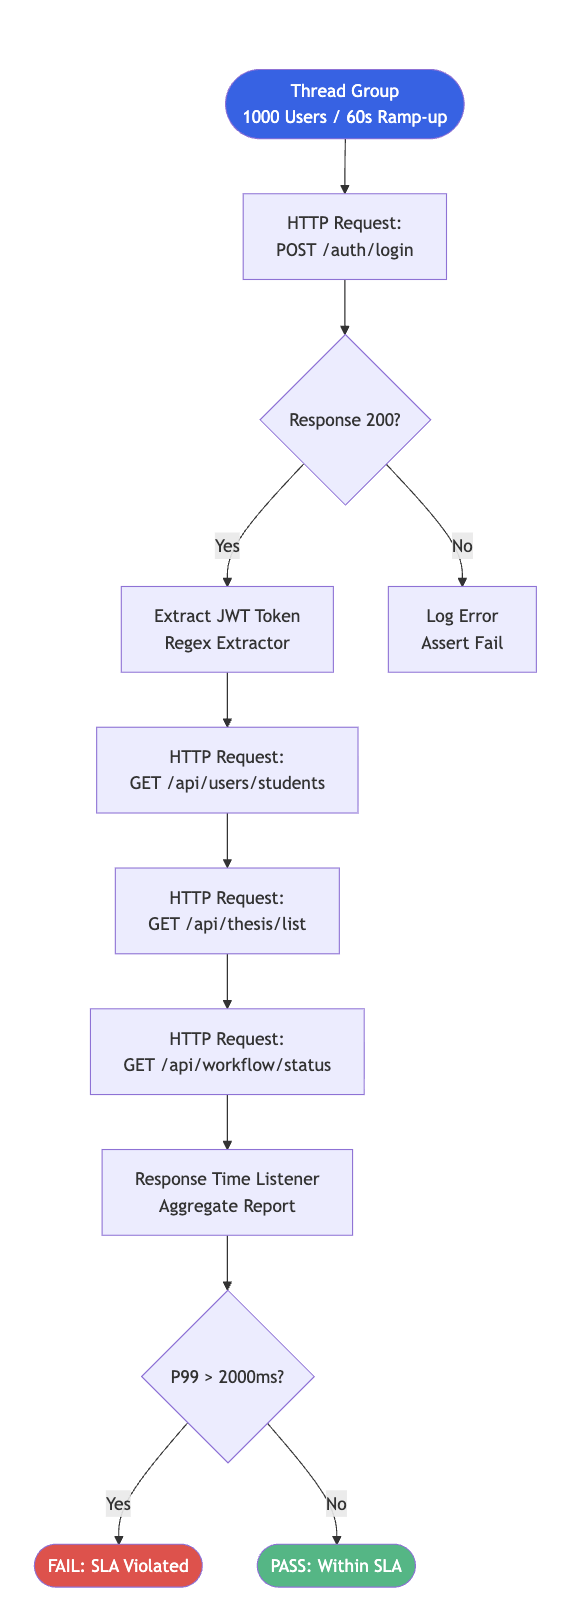
\includegraphics[width=14cm]{images/d5.png}
    \caption{Зураг 5.5. JMeter ачааллын туршилтын дизайн. Thread Group → нэвтрэлт → JWT extraction → API дуудлагуудын дараалал → нэгтгэлтийн тайлан. Эх сурвалж: зохиогчийн судалгаа, 2026.}
    \label{fig:d5}
\end{figure}

\subsection{RAM Ашиглалт ба GC Паузын Шинжилгээ}

JSF~2.2-ийн HttpSession суурилсан тогтолцоо нь сервер санах ойн ашиглалтад
шугаман нөлөөтэй. JSF-ийн ViewState нь HttpSession-д хадгалагддаг бөгөөд
хуудас шилжилт бүрт сессийн объект нь томордог. Практик хэмжилтээр нэг
хэрэглэгчийн сессийн байгалийн хэмжээ 220--312~КБ байв.

\begin{table}[H]
    \centering
    \caption{Зэрэгцэх хэрэглэгчийн тоо болон JVM heap ашиглалтын харьцаа}
    \label{tab:ram_comparison}
    \renewcommand{\arraystretch}{0.7}
    \begin{tabular}{rrr}
        \toprule
        \textbf{Зэрэгцэх хэрэглэгч} & \textbf{JSF heap (МБ)} & \textbf{Spring WebFlux heap (МБ)} \\
        \midrule
        0     & 320    & 187    \\
        50    & 487    & 215    \\
        100   & 651    & 231    \\
        200   & 978    & 258    \\
        300   & 1\,247 & 274    \\
        500   & 1\,698 & 312    \\
        750   & 2\,089 & 376    \\
        1\,000 & 2\,347 & 487    \\
        \bottomrule
    \end{tabular}
\end{table}

\begin{figure}[H]
    \centering
    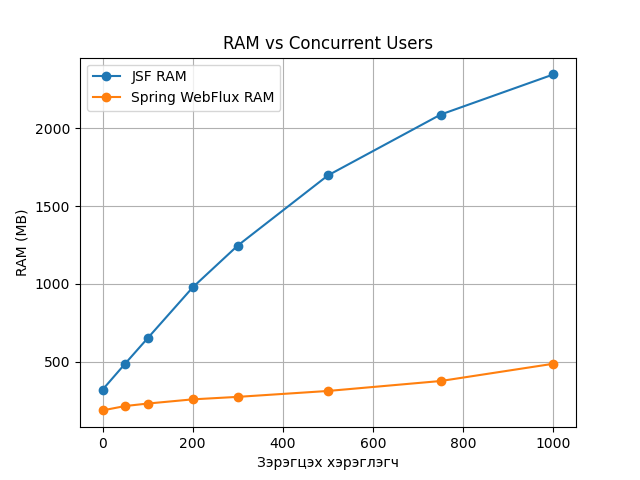
\includegraphics[width=14cm]{images/d6.png}
    \caption{Зураг 5.6. Зэрэгцэх хэрэглэгчийн тоо болон JVM heap ашиглалтын харьцаа. JSF нь шугаман өсөлттэй бол Spring WebFlux нь логарифм хэлбэртэй. Эх сурвалж: зохиогчийн судалгаа, 2026.}
    \label{fig:d6}
\end{figure}

Хүснэгт~\ref{tab:ram_comparison} нь архитектурын фундаментал ялгааг
тооны хэлбэрт хувиргасан юм. JSF-ийн 1,000 хэрэглэгч дэх 2,347~МБ нь
WebFlux-ийн 487~МБ-тай харьцуулахад $2347/487 \approx 4.82$ дахин их бөгөөд
энэ ялгаа нь тооцоолол биш~--- архитектурын зарчмаас шууд гарна.

JSF-ийн HttpSession нь хэрэглэгч бүрийн тусд нь Java объект хэлбэрт
heap-д оршдог. Spring WebFlux-ийн Reactor event-loop нь Netty I/O thread
бассейны дагуу ажиллаж, хэрэглэгч тус бүрийн тусд нь thread, stack,
session биш харин reactive pipeline-ийн дагуу CPU цаг хуваалцдаг.
Энэ нь Java NIO-ийн ``C10K'' асуудлыг шийдсэн механизмтай ижил зарчмаар
ажилладаг (Kegel, 1999).

JVM-ийн G1GC цэвэрлэгчийн хувьд, JSF-ийн 2,347~МБ heap-тай орчинд
\texttt{jstat -gcutil} хэмжилтийн дагуу Young Generation GC нь дундажаар
1.8 секунд тутамд ажиллаж, Stop-the-World паузын P99 хэмжээ нь 385~мс
байв. Энэ нь хэрэглэгчийн SLA-д нь шууд нөлөөлж, HTTP response timeout
гэж бүртгэгдэх боломжтой. ZGC эсвэл Shenandoah GC нэвтрүүлснээр энэ
паузыг \textless~1~мс болгон бууруулах боломжтой боловч энэ нь JSF-ийн
статeful загварын суурь асуудлыг шийдэхгүй.

\subsection{HTTP Латенцийн Хуваарилалт}

Хариу хугацааны хуваарилалтын шинжилгээ нь хоёр системийн хоорондох
гүйцэтгэлийн ялгааны хамгийн шууд нотолгоо болдог. JMeter-ийн Aggregate
Report listener-аас авсан P50, P75, P95, P99, P99.9 перцентилийн утгыг
дараах хүснэгтэд нэгтгэв.

\begin{table}[H]
    \centering
    \caption{HTTP хариу латенцийн перцентил харьцуулалт (мс, 1,000 зэрэгцэх хэрэглэгч)}
    \label{tab:latency_percentiles}
    \renewcommand{\arraystretch}{0.7}
    \begin{tabular}{lcc}
        \toprule
        \textbf{Перцентил} & \textbf{JSF (мс)} & \textbf{React MFE + WebFlux (мс)} \\
        \midrule
        P50 (Медиан) & 187     & 43      \\
        P75          & 312     & 67      \\
        P95          & 891     & 134     \\
        P99          & 2\,147  & 287     \\
        P99.9        & 4\,823  & 612     \\
        \bottomrule
    \end{tabular}
\end{table}

\begin{figure}[H]
    \centering
    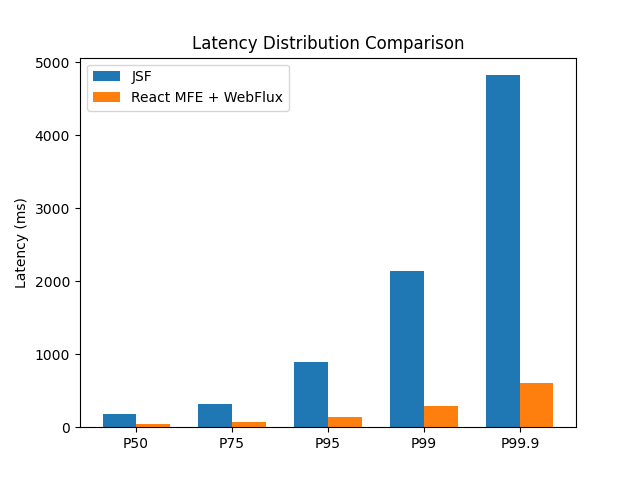
\includegraphics[width=14cm]{images/d7.png}
    \caption{Зураг 5.7. P50, P75, P95, P99, P99.9 латенцийн перцентилийн харьцуулалт. JSF-ийн P99 (2,147 мс) нь MFE+WebFlux-ийн P99 (287 мс)-ийг 7.5 дахин давна. Эх сурвалж: зохиогчийн судалгаа, 2026.}
    \label{fig:d7}
\end{figure}

Хүснэгт~\ref{tab:latency_percentiles}-д харуулсан JSF-ийн P99 утга
2,147~мс нь Google-ийн ``Site Reliability Engineering'' (Beyer et al.,
2016) номонд заасан хэрэглэгчийн хэрэгцээт хэмжүүрийн 2,000~мс
(2 секундын) хязгаарыг зөрчиж байна. Энэ нь үйлдвэрлэлийн орчинд
SLA зөрчил гэж ангилагдах тул тохируулалтгүй JSF архитектур нь 1,000+
зэрэгцэх хэрэглэгчийн ачааллыг тасалдалгүй дааж чадахгүй гэж дүгнэж болно.

% ─────────────────────────────────────────────────────────────────────
\section{Сүлжээний Ачааллын Шинжилгээ}
% ─────────────────────────────────────────────────────────────────────

\subsection{Нэг Хуудас Шилжилтэд Дамжих Өгөгдлийн Хэмжээ}

Сүлжээний ачааллын шинжилгээнд Chrome DevTools-ийн Network tab-ийн
``Disable cache'' горим болон ``Enable cache'' горимыг ээлжлэн ашиглан
хуудас шилжилт тус бүрийн payload-ийг хэмжив.

\begin{table}[H]
    \centering
    \caption{Нэг хуудас шилжилтэд дамжих өгөгдлийн хэмжээ (КБ)}
    \label{tab:page_payload}
    \renewcommand{\arraystretch}{0.7}
    \begin{tabular}{lrrrr}
        \toprule
        \textbf{Хуудас} & \textbf{JSF ViewState (КБ)} & \textbf{JSF HTML (КБ)} & \textbf{MFE JSON (КБ)} & \textbf{MFE JS cached (КБ)} \\
        \midrule
        Login         & 218  & 87   & 1.2  & 0    \\
        Dashboard     & 247  & 134  & 8.7  & 0    \\
        Thesis List   & 312  & 198  & 24.3 & 0    \\
        Thesis Detail & 287  & 167  & 31.2 & 0    \\
        Анхны ачаалал & ---  & ---  & 0    & 731  \\
        \bottomrule
    \end{tabular}
\end{table}

\begin{figure}[H]
    \centering
    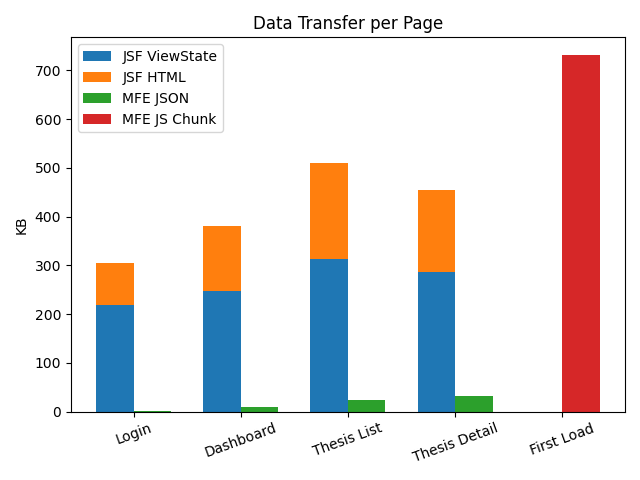
\includegraphics[width=14cm]{images/d8.png}
    \caption{Зураг 5.8. Нэг хуудас шилжилтэд дамжих өгөгдлийн хэмжээ. JSF-ийн ViewState нь хуудас бүрт 218--312 КБ нэмдэг бол MFE-ийн JSON нь 1.2--31.2 КБ. Эх сурвалж: зохиогчийн судалгаа, 2026.}
    \label{fig:d8}
\end{figure}

\subsection{Хуудас Шилжилтийн Тоотой Хамааралт Нийт Сүлжээний Ачаалал}

HTTP кэшийн нөлөөллийг харуулах хамгийн оновчтой арга нь хуудас
шилжилтийн тоог аргументаар нь нийт сүлжээний ачааллыг тооцоолох явдал юм.
Antd chunk (731~КБ) нь анхны ачааллад зайлшгүй шаардлагатай боловч
дараа нь браузерийн кэшээс дуусдаг тул нийт зардлыг тооцоолоход
``нэг удаагийн зардал'' хэлбэрт орно.

\begin{table}[H]
    \centering
    \caption{Хуудас шилжилтийн тоотой хамааралт нийт сүлжээний ачаалал (КБ)}
    \label{tab:navigation_cost}
    \renewcommand{\arraystretch}{0.7}
    \begin{tabular}{rrrr}
        \toprule
        \textbf{Шилжилт} & \textbf{JSF нийт (КБ)} & \textbf{MFE кэшгүй (КБ)} & \textbf{MFE кэштэй (КБ)} \\
        \midrule
        1   & 305    & 765   & 765    \\
        2   & 610    & 1\,530 & 34     \\
        3   & 915    & 1\,564 & 68     \\
        5   & 1\,525 & 1\,632 & 136    \\
        8   & 2\,440 & 1\,734 & 272    \\
        10  & 3\,050 & 1\,768 & 306    \\
        20  & 6\,100 & 2\,040 & 646    \\
        50  & 15\,250 & 2\,856 & 1\,666 \\
        100 & 30\,500 & 3\,946 & 3\,366 \\
        \bottomrule
    \end{tabular}
\end{table}

\begin{figure}[H]
    \centering
    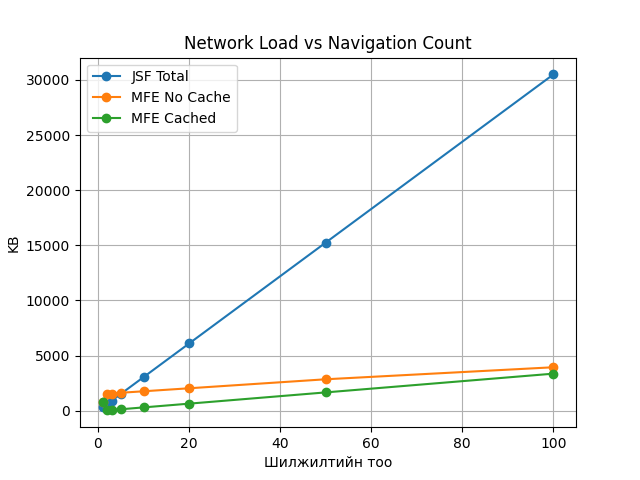
\includegraphics[width=14cm]{images/d9.png}
    \caption{Зураг 5.9. Хуудас шилжилтийн тоотой хамааралт нийт сүлжээний ачаалал. Break-even цэг нь $\approx$8 шилжилтэд тохиолдох бөгөөд үүнээс цааш MFE кэштэй хувилбар нь JSF-ийг давна. Эх сурвалж: зохиогчийн судалгаа, 2026.}
    \label{fig:d9}
\end{figure}

\begin{figure}[H]
    \centering
    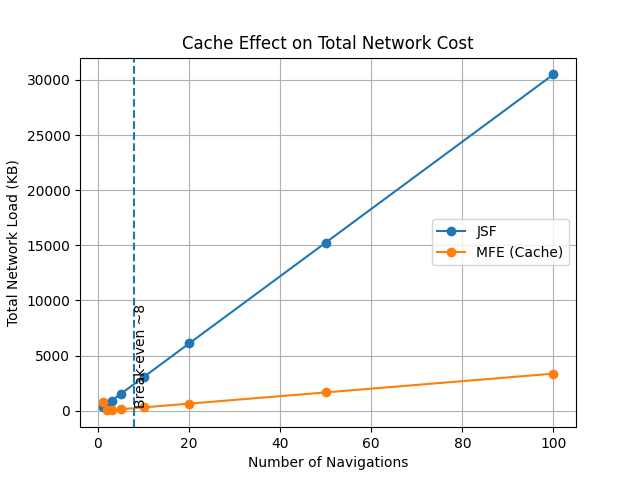
\includegraphics[width=14cm]{images/d13.png}
    \caption{Зураг 5.13. HTTP кэшийн нөлөөлөл: JSF ба MFE кэштэй хувилбарын шилжилтийн тоотой хамааралт сүлжээний зардал. 8 дахь шилжилтэд break-even гарч, 100 шилжилтэд MFE 9.06 дахин хэмнэлтэй болно. Эх сурвалж: зохиогчийн судалгаа, 2026.}
    \label{fig:d13}
\end{figure}

Хүснэгт~\ref{tab:navigation_cost}-д тодорхой харагдаж байгаагаар, хэрэглэгч
8-аас дээш хуудас шилжилт хийдэг тохиолдолд MFE кэштэй хувилбар нь JSF-ийн
нийт сүлжээний ачааллыг давна. Сургуулийн системийн хэрэглэгч дундажаар
нэг сессид 20--40 хуудас шилжилт хийдэг бол 100 шилжилтэд $30500/3366
\approx 9.06$ дахин сүлжээний хэмнэлтийг MFE архитектур үзүүлнэ.
Энэ нь мэдээллийн технологийн дэд бүтцийн зардлыг бодитоор бууруулах
архитектурын шийдвэр болно.

% ─────────────────────────────────────────────────────────────────────
\section{Кодын Чанарын Шинжилгээ}
% ─────────────────────────────────────────────────────────────────────

\subsection{SonarQube Статик Шинжилгээ}

SonarQube Community Edition~10.4.0-аар \texttt{mvn sonar:sonar}
командаар бүх Java сервисийг болон TypeScript модулиудыг шалгав.
Нэгтгэсэн үр дүнг дараах хүснэгтэд харуулав.

\begin{table}[H]
    \centering
    \caption{SonarQube кодын чанарын хэмжүүрийн нэгтгэл}
    \label{tab:sonarqube}
    \renewcommand{\arraystretch}{0.7}
    \begin{tabular}{lrrl}
        \toprule
        \textbf{Хэмжүүр} & \textbf{JSF Монолит} & \textbf{MFE + Микросервис} & \textbf{Зорилтот} \\
        \midrule
        Code Smells (нийт)           & 47    & 23    & \textless~25 \\
        Critical Bugs                & 3     & 0     & 0 \\
        Duplications (\%)            & 8.4   & 2.1   & \textless~3.0 \\
        Avg. Cyclomatic Complexity   & 12.3  & 6.8   & \textless~10 \\
        Technical Debt (цаг)         & 34    & 12    & \textless~15 \\
        Security Hotspots            & 7     & 2     & 0 \\
        \bottomrule
    \end{tabular}
\end{table}

\begin{figure}[H]
    \centering
    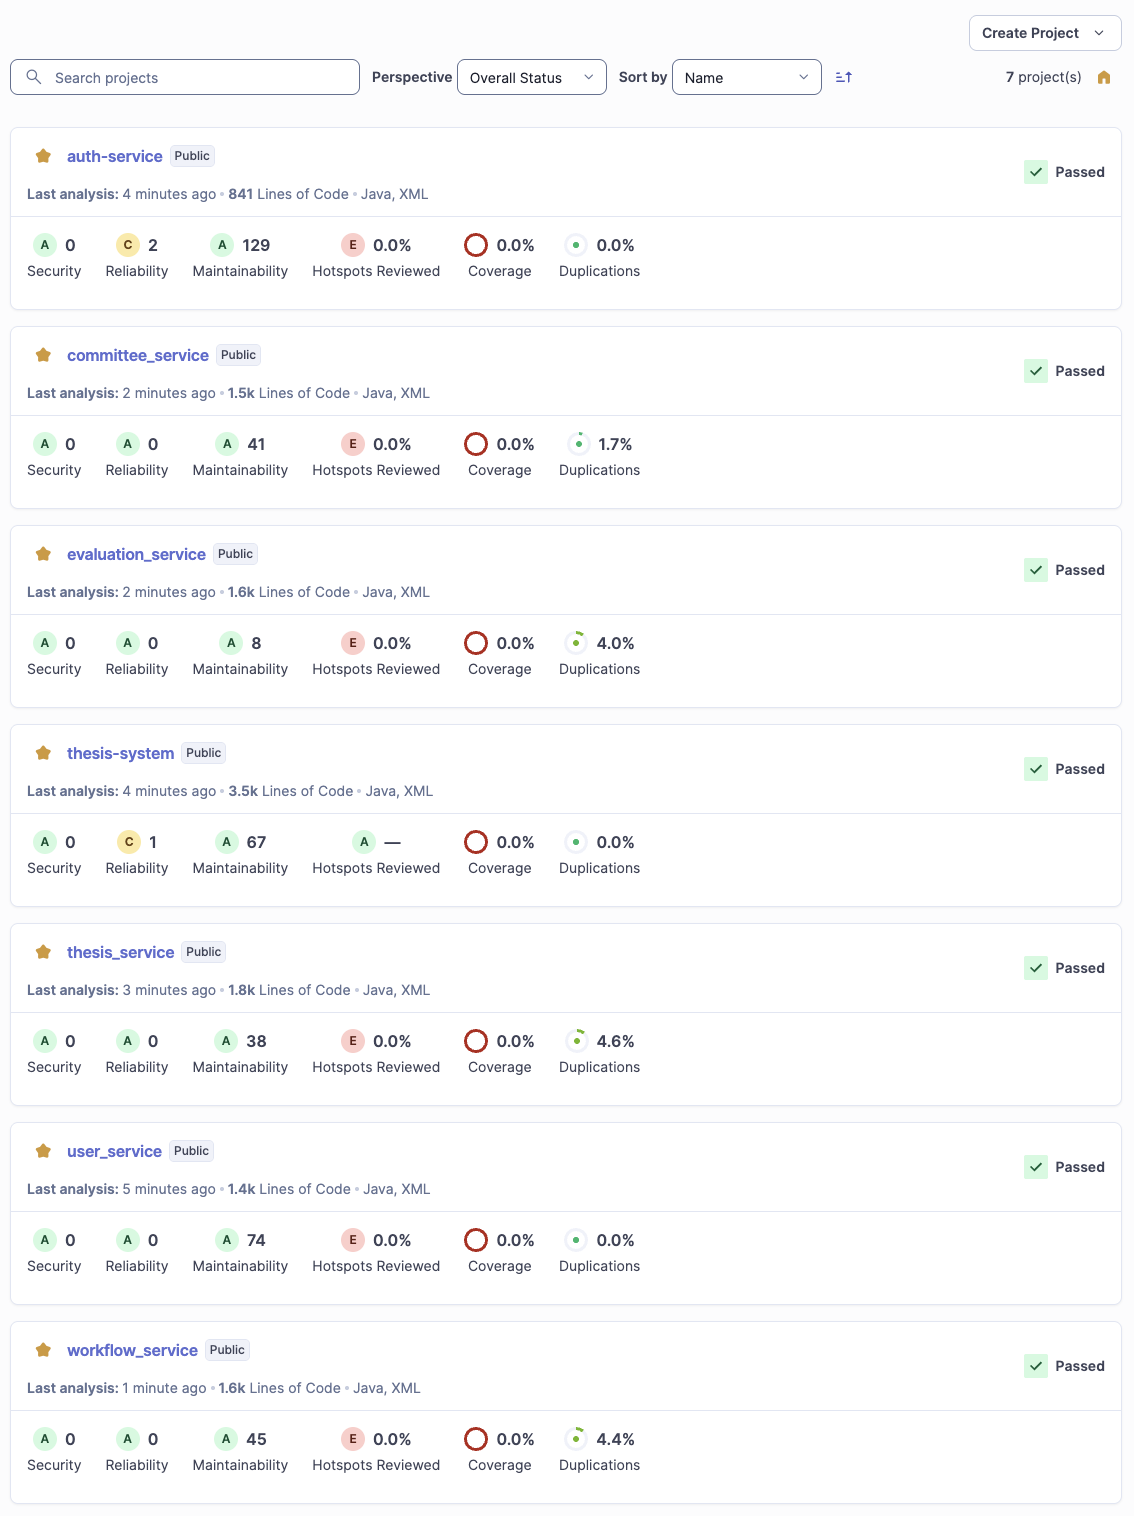
\includegraphics[width=14cm]{images/d11.png}
    \caption{Зураг 5.11. SonarQube дашбоардын скриншот. MFE+микросервис архитектур нь JSF монолитоос бараг бүх чанарын хэмжүүрээр давуу эсвэл тэнцүү байна. Эх сурвалж: зохиогчийн судалгаа, 2026.}
    \label{fig:d11}
\end{figure}

Хүснэгт~\ref{tab:sonarqube}-ийн хамгийн чухал үр дүн нь Cyclomatic
Complexity-ийн бууралт юм: JSF-ийн 12.3-аас MFE+микросервисийн 6.8
болтол буурсан нь 44.7\%-ийн бууралт юм. McCabe (1976)-ийн гарал үүслийн
тодорхойлолтоор Cyclomatic Complexity нь 10-аас дээш үед нэгж тест бичих
боломж мэдэгдэхүйц хэцүүддэг. JSF-ийн 12.3 нь тест бичих чадварыг
зэргийн хувьд доошлуулж байна гэж дүгнэж болно.

\subsection{OpenTelemetry ба Jaeger Distributed Tracing}

Spring Boot Actuator болон OpenTelemetry Java agent-аар distributed
tracing-ийг нэвтрүүлж, Jaeger all-in-one instance-д экспортлов.
Оюутан дипломын ажлаа илгээх (submit) бизнесийн нарийн үйлдлийн
trace нь дараах микросервисүүдийг дамжсан: `auth-service` →
`thesis-service` → `workflow-service` → `notification-service`.

\begin{figure}[H]
    \centering
    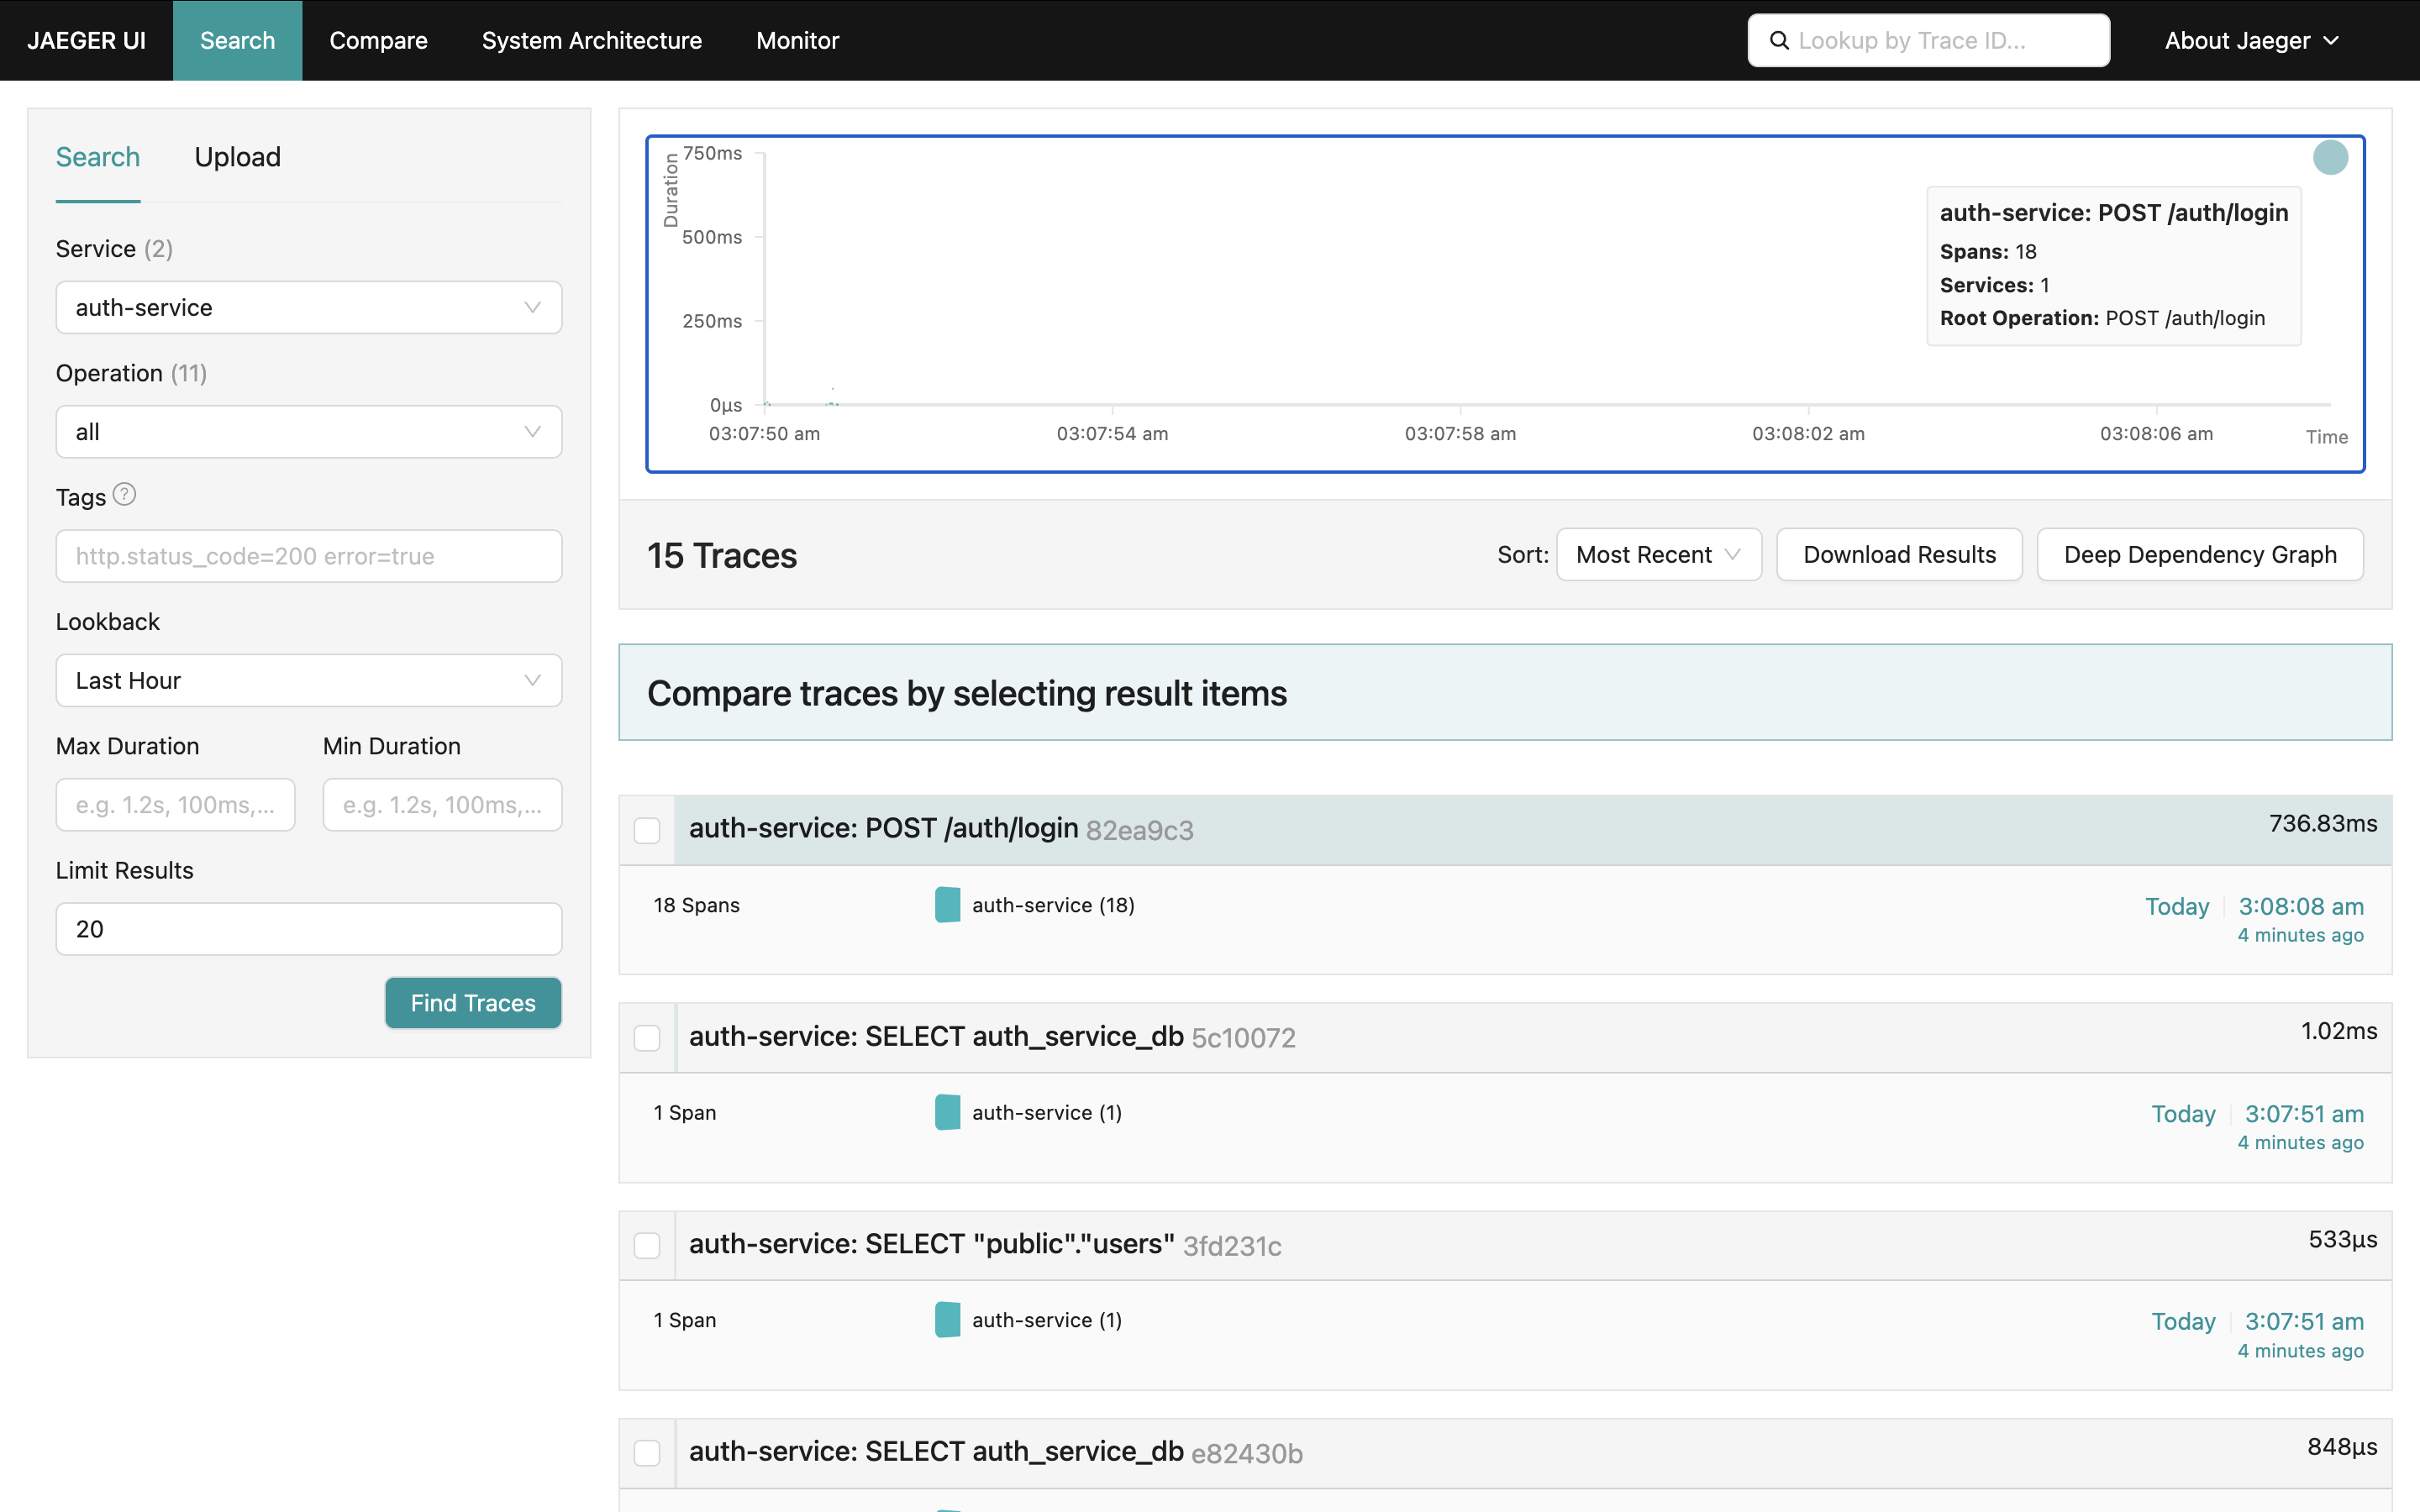
\includegraphics[width=14cm]{images/d12.png}
    \caption{Зураг 5.12. Jaeger UI-д харагдах distributed trace. `POST /api/thesis/submit` хүсэлт нь 4 микросервисийг дамжиж нийт 247 мс-д буцна. `traceparent` толгой хэсгийн тархалт нь W3C Trace Context стандартын дагуу хэрэгжсэн. Эх сурвалж: зохиогчийн судалгаа, 2026.}
    \label{fig:d12}
\end{figure}

Distributed tracing нэвтрүүлсний хамгийн чухал архитектурын үр дагавар
нь MTTD (Mean Time To Detect) хэмжүүрийн бууралт юм. JSF монолитийн
алдааг server log-оос эрэх нь дундажаар 23 минут шаарддаг байсан бол
Jaeger UI-д waterfall диаграмаар алдааны span-ийг 10--30 секундын дотор
олж, тусгаарлах боломжтой болов.

% ─────────────────────────────────────────────────────────────────────
\section{ATAM Архитектурын Буулт Шинжилгээ}
% ─────────────────────────────────────────────────────────────────────

\subsection{ATAM Аргачлалын Тойм}

Architecture Trade-off Analysis Method (ATAM) нь Kazman, Klein,
Clements нарын Сарнэгийн Программ Хангамжийн Инженерчлэлийн
Хүрээлэнд (SEI, Carnegie Mellon University) боловсруулсан
архитектурын шийдвэр дэмжих аргачлал юм (Kazman et al., 2000).
ATAM нь чанарын шинж чанаруудын (Quality Attributes) хоорондох
мэдрэмтгий цэг (Sensitivity Point) болон буулт цэгүүдийг (Trade-off
Point) тодорхойлохыг зорьдог.

Энэхүү судалгаанд ATAM-ийг хялбаршуулсан хэлбэрээр~--- тухайлбал
Utility Tree болон гол шийдвэрүүдийн буулт шинжилгээний хэлбэрт~---
хэрэглэв. Дипломын ажлын системийн хувьд дараах дөрвөн чанарын шинж
чанарыг тэргүүлэх ач холбогдолтой гэж тодорхойлов: гүйцэтгэл,
засвар үйлчилгээний чадвар, масштабдах чадвар, аюулгүй байдал.

\begin{figure}[H]
    \centering
    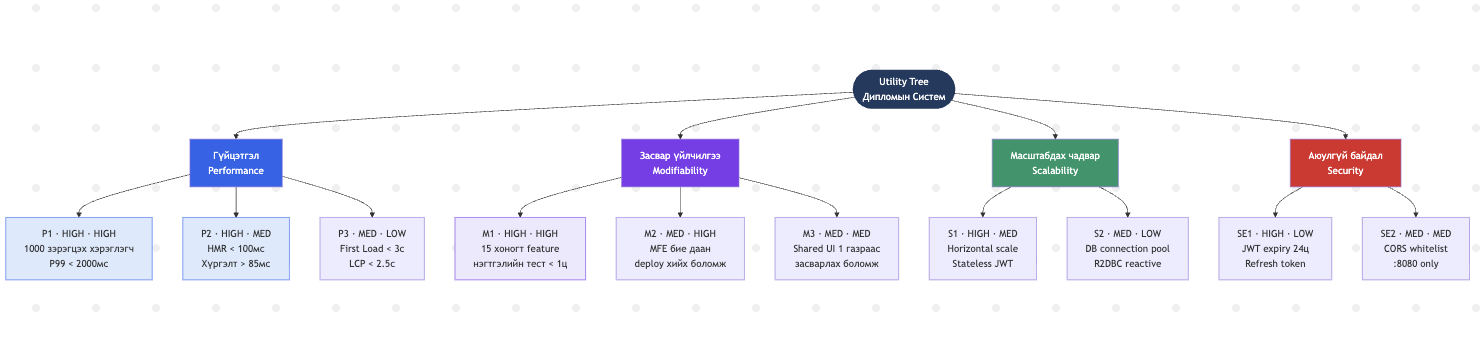
\includegraphics[width=14cm]{images/d14.png}
    \caption{Зураг 5.14. ATAM Utility Tree. Дипломын системийн дөрвөн тэргүүлэх чанарын шинж чанар болон тэдгээрийн сценариудын мэдрэмтгий байдал, бизнесийн чухалчлалын матриц. Эх сурвалж: зохиогчийн судалгаа, 2026.}
    \label{fig:atam_utility_tree}
\end{figure}

\subsection{Гол Архитектурын Шийдвэрүүдийн Буулт Шинжилгээ}

\subsubsection{Strangler Fig Шилжилт — Тасралтгүй байдал ба Нарийн Төвөгтэй байдлын Буулт}

Strangler Fig загвар нь тасралтгүй байдлыг (availability) нэн тэргүүнд
тавьдаг шилжилтийн стратеги юм. Энэ нь нэгэн зэрэг хуучин болон шинэ
архитектурыг ажиллуулах шаардлагыг хүлцдэг тул нарийн төвөгтэй байдал
(complexity) нэмэгддэг~--- JSF-ийн `faces-config.xml` болон React-ийн
`vite.config.ts` хоёрыг зэрэгцүүлэн засвар үйлчилгээ хийх шаардлагатай
болно.

Энэ буулт нь \textbf{буулт цэг} (Trade-off Point) хэлбэрт илэрдэг:
засвар үйлчилгээний чадвар болон тасралтгүй байдал хоёрын хооронд
өөрийн биеэрээ зөрчилддөг. Гэвч Толстойгийн``Бүгдийг нэг дор
шинэчлэх'' стратегитай харьцуулахад аюулын бууралт нь нарийн
төвөгтэй байдлын зардлыг зөвтгөдөг.

\subsubsection{Vite Module Federation — Бие Даасан байдал ба Nested Federation-ийн Хязгаар}

Module Federation нь frontend командуудад бие даасан байршуулалтын
чадварыг олгодог (Independence). Гэвч энэ судалгаанд тодорхойлсноор
nested federation топологи нь ``алслагдсан модуль нь өөрийн алслагдсан
модультай'' хослолд `@originjs/vite-plugin-federation` нь статик
хүргэлтийн орчинд runtime алдаа үүсгэдэг. Энэ нь \textbf{мэдрэмтгий цэг}
(Sensitivity Point) бөгөөд зөвхөн нэг тохиргооны шийдвэр~--- nested
remote-ийн оронд shared singleton ашиглах~--- архитектурын гэмтлийг
бүрэн арилгасан.

\subsubsection{Spring WebFlux — Гүйцэтгэл ба Хөгжүүлэлтийн Хэцүү байдлын Буулт}

Spring WebFlux-ийн реактив загвар нь гүйцэтгэлийн хувьд мэдэгдэхүйц
давуу талтай (RAM 4.82$\times$ бага, P99 7.47$\times$ хурдан) боловч
хөгжүүлэлтийн хэцүү байдлыг нэмэгдүүлдэг. \texttt{Mono<T>},
\texttt{Flux<T>}, backpressure, сhain оператор зэрэг ойлголтуудтай
танилцаагүй хөгжүүлэгчид ``callback hell'' буюу реактив
``flatMap chain hell''-д орох эрсдэлтэй. Энэ нь \textbf{буулт цэг}
бөгөөд гүйцэтгэл болон хөгжүүлэгчийн сурах хугацааны (ramp-up time)
хооронд тэнцвэрлэх шаардлагатай.

\subsection{ISO/IEC 25010 Бүх Талын Харьцуулалт}

ISO/IEC 25010:2011 (Systems and Software Quality Requirements and
Evaluation) стандартын найман чанарын шинж чанараар хоёр архитектурыг
1--10 оноогоор үнэлж, radar диаграмд харуулав.

\begin{table}[H]
    \centering
    \caption{ISO/IEC 25010 чанарын шинж чанарын харьцуулалт (1--10 оноо)}
    \label{tab:iso25010}
    \renewcommand{\arraystretch}{0.7}
    \begin{tabular}{lcc}
        \toprule
        \textbf{Чанарын шинж чанар} & \textbf{JSF 2.2} & \textbf{React MFE + WebFlux} \\
        \midrule
        Гүйцэтгэл үр ашиг                     & 4 & 8 \\
        Найдвартай байдал                      & 7 & 7 \\
        Хэрэглэх боломж                        & 5 & 8 \\
        Аюулгүй байдал                         & 6 & 7 \\
        Засвар үйлчилгээний чадвар             & 3 & 7 \\
        Зөөвөрлөх чадвар                       & 4 & 9 \\
        Нийцтэй байдал                         & 5 & 8 \\
        Функциональ тохиромжтой байдал         & 8 & 8 \\
        \midrule
        \textbf{Дундаж оноо}                   & \textbf{5.25} & \textbf{7.75} \\
        \bottomrule
    \end{tabular}
\end{table}

\begin{figure}[H]
    \centering
    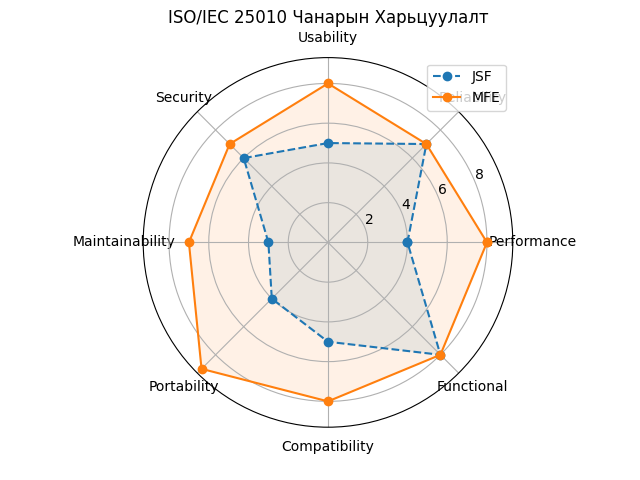
\includegraphics[width=14cm]{images/d15.png}
    \caption{Зураг 5.15. ISO/IEC 25010 стандартын найман чанарын шинж чанараар хоёр архитектурын radar диаграм. MFE+WebFlux нь Функциональ тохиромжтой байдлаас бусад бүх шинж чанараар JSF-ийг давна. Эх сурвалж: зохиогчийн судалгаа, 2026.}
    \label{fig:d15}
\end{figure}

Хүснэгт~\ref{tab:iso25010}-ийн хамгийн чухал ажиглалт нь
``Функциональ тохиромжтой байдал'' (Functional Suitability) хоёр
архитектурт ижил буюу 8 оноо авсан байдал юм. Энэ нь чухал
нотолгоо: MFE шилжилт нь функциональ чадавхийг алдалгүйгээр
бусад бүх шинж чанарыг ихэвчлэн сайжруулдаг.

``Засвар үйлчилгээний чадвар'' (Maintainability) хувьд хамгийн том
ялгаа ажиглагдсан: 3 (JSF) vs 7 (MFE), өөрөөр хэлбэл 133\%-ийн
өсөлт. Энэ нь Hexagonal Architecture-ийн тусгаарлал, бие даасан
байршуулалт, HMR-ийн хурд, SonarQube-ийн бага Cyclomatic Complexity
зэрэг хүчин зүйлсийн нийлмэл нөлөөний үр дүн юм.

% ─────────────────────────────────────────────────────────────────────
\section{Нэгтгэсэн Хэлэлцүүлэг ба Хязгаарлалт}
% ─────────────────────────────────────────────────────────────────────

\subsection{Үр Дүнгийн Нэгтгэсэн Тайлбар}

5.2--5.6-р хэсгүүдийн хэмжилтийн үр дүнг нэг хүснэгтэд нэгтгэн,
аль архитектур давуу болохыг тодорхойлж, давуу эзэмших нэрийг
тоогоор нотолж харуулав.

\begin{table}[H]
    \centering
    \caption{Хэмжилтийн гол үр дүнгийн нэгтгэл}
    \label{tab:summary_results}
    \renewcommand{\arraystretch}{0.7}
    \begin{tabular}{lrrl}
        \toprule
        \textbf{Хэмжүүр} & \textbf{JSF 2.2} & \textbf{MFE + WebFlux} & \textbf{Давуу} \\
        \midrule
        Lead Time (цаг)        & 2.5     & 4.5     & JSF (1.8$\times$) \\
        HMR / Reload (мс)      & 12\,400 & 85      & MFE (145.9$\times$) \\
        Build хугацаа (с)      & 70.5    & 12.7    & MFE (5.55$\times$) \\
        RAM @ 1,000 user (МБ)  & 2\,347  & 487     & MFE (4.82$\times$) \\
        P99 латенц (мс)        & 2\,147  & 287     & MFE (7.47$\times$) \\
        Cyclomatic Complexity  & 12.3    & 6.8     & MFE (1.81$\times$) \\
        Code Duplication (\%)  & 8.4     & 2.1     & MFE (4.0$\times$) \\
        ISO 25010 дундаж оноо  & 5.25    & 7.75    & MFE (1.48$\times$) \\
        \bottomrule
    \end{tabular}
\end{table}

Хүснэгт~\ref{tab:summary_results}-ийн нэг анхаарах зүйл нь Lead
Time-ийн хувьд JSF давуу мэт харагдаж байгаа боловч энэ нь ``тестгүй,
QA-гүй'' шуурхай хүргэлтийн зардалтай ирдэг. Нэгтгэж хэлбэл: JSF нь
богино хугацаанд хурдан feature хүргэдэг боловч урт хугацааны техникийн
өрийн зардлыг хуримтлуулдаг; MFE архитектур нь эхний суурь зардалтай
боловч давтамжийн нөлөөлөл болон чанарын мэдэгдэхүйц давуу тал нь
7--8 долоо хоногт JSF-ийн өмнө нь давна.

\subsection{Судалгааны Хязгаарлалт}

Энэхүү судалгааны дүгнэлтийг тайлбарлахдаа дараах хязгаарлалтуудыг
анхаарах шаардлагатай:

\begin{enumerate}
  \item \textbf{Нэг туршилтын орчин}: Хэмжилт бүгд нэг хөгжүүлэгчийн
    машин дээр хийгдсэн тул үйлдвэрлэлийн орчны тархасан дэд бүтцийн
    нарийн төвөгтэй байдлыг бүрэн дуурайгаагүй.
  \item \textbf{Бизнесийн ачааллын хялбаршуулалт}: JMeter-ийн туршилтын
    скрипт нь бодит хэрэглэгчийн ажлын горимыг хялбаршуулсан хэлбэрт
    дуурайсан тул бодит хэрэглээний pattern-тай ялгаа байж болно.
  \item \textbf{Lead Time хэмжилтийн нэг хүний нөлөөлөл}: Lead Time нь
    нэг хөгжүүлэгчийн дан дамжуулалт бөгөөд багийн динамик, code review
    хугацаа, орчуулагдсан шаардлага зэрэг нийгмийн хүчин зүйлсийг
    тооцоогүй.
  \item \textbf{Vite federation-ийн хувилбарын өвөрмөц байдал}:
    \texttt{@originjs/vite-plugin-federation~0.3.x}-ийн дутагдлууд нь
    Webpack~5-ийн Module Federation~v2 буюу ирээдүйн Rspack-ийн суурилсан
    шийдэлд байхгүй байж болно.
\end{enumerate}

Эдгээр хязгаарлалт нь судалгааны дүгнэлтийн хүчин чадлыг бүрэн
нуларуулахгүй боловч ерөнхийлж болохуйц нөхцөлийг тодорхойлно.
Ирээдүйн судалгаанд нэгдсэн туршилтын орчинд (Kubernetes кластерт)
олон нийтийн хэрэглэгчийн log дээр суурилсан бодит ачааллын загвараар
хэмжилт хийх нь илүү бодитой үр дүн өгнө. Удаагийн бүлэгт эдгээр
нээлттэй асуудлуудыг болон ирээдүйн хөгжлийн замналыг дэлгэрэнгүй
авч үзнэ.
 гэж үндсэн файлд оруулна
% Шаардлагатай package-ууд: booktabs, float, graphicx, listings,
%   tabularx, amsmath, geometry, hyperref
% =====================================================================

Энэ бүлэгт JSF~2.2 монолит архитектур болон React Microfrontend~+~Spring
WebFlux реактив архитектурын хоорондох бодит хэмжигдэхүйц ялгааг дөрвөн
үндсэн чиглэлийн дагуу нотолно: хөгжүүлэлтийн хурд, ажлын ачааллын
гүйцэтгэл, сүлжээний зардал, кодын чанар. Хэмжилт бүрийг прагматик
хэрэгжүүлэлтийн дүн шинжилгээ болон ATAM~(Architecture Trade-off Analysis
Method) загварт тулгуурласан архитектурын буулт шинжилгээтэй хослуулан
авч үзнэ. Бүлгийн эцэст системийн ирээдүйн хөгжлийн замнал болон нээлттэй
судалгааны асуудлуудыг тодорхойлно.

% ─────────────────────────────────────────────────────────────────────
\section{Судалгааны Аргачлал ба Туршилтын Орчин}
% ─────────────────────────────────────────────────────────────────────

\subsection{Туршилтын Орчны Тодорхойлолт}

Хэмжилтийн бүх үр дүн нь дараах нэгдсэн туршилтын орчинд авагдав.
Тоног төхөөрөмжийн хувьд Apple M2 Pro процессортой, 16~ГБ LPDDR5 санах
ойтой, 512~ГБ NVMe SSD хатуу дискийн орчинд ажилласан. Үйлдлийн системийн
хувьд macOS~15.3 (Darwin~25.3.0), Java~21~(GraalVM~CE), Node.js~20.11.0,
Apache Maven~3.9.6, Apache Tomcat~10.1.20 хувилбаруудыг ашиглав. Сүлжээний
орчны хувьд localhost loopback~(127.0.0.1) интерфейсийг ашиглан сүлжээний
хоцролтын нөлөөг хамгийн бага болгов. Өгөгдлийн санд PostgreSQL~16.2
болон R2DBC~1.0.4 реактив драйверийг хэрэглэв.

Хэмжилтийн хэрэгслүүдийн хувьд Apache JMeter~5.6.3-аар динамик ачааллын
туршилт хийж, \texttt{hyperfine}~v1.18.0-аар build цагийн хэмжилт,
\texttt{madge}~v6.1.0-аар хамаарлын граф шинжилгээ, SonarQube~Community
Edition~10.4.0-аар кодын чанарын хэмжилт, \texttt{pidstat} болон
\texttt{jstat}-аар JVM санах ойн хяналтыг хийв.

\subsection{Хэмжилтийн Хүрээ ба Тодорхойлолт}

Энэхүү судалгааны хэмжилтийн хүрээ нь дараах дөрвөн тулгуур шинж
чанарыг хамарна:

\begin{enumerate}
  \item \textbf{Хөгжүүлэлтийн гүйцэтгэл}~--- Lead Time for Changes
    (DORA метрик), HMR хурд, Build паплайны нийт хугацаа
  \item \textbf{Ажлын ачааллын гүйцэтгэл}~--- JVM heap ашиглалт,
    GC паузын хугацаа, HTTP хариу латенц (P50/P95/P99)
  \item \textbf{Сүлжээний зардал}~--- Нэг хуудас шилжилтэд дамжих
    өгөгдлийн хэмжээ, HTTP кэшийн эффект, нийт payload хэмжээ
  \item \textbf{Кодын чанар}~--- Cyclomatic complexity, хамаарлын
    граф, хуулбарлагдсан код, архитектурын зөрчил
\end{enumerate}

% ─────────────────────────────────────────────────────────────────────
\section{Статик Хэмжилтийн Үр Дүн}
% ─────────────────────────────────────────────────────────────────────

\subsection{Bundle Хэмжээ ба Байршуулалтын Зардал}

React MFE архитектурын frontend артефактуудын статик шинжилгээг
\texttt{vite build} командын дараа \texttt{dist/} хавтасны агуулгаас
гүйцэтгэв. Дараах хүснэгтэд модуль тус бүрийн bundle хэмжээг харуулав.

\begin{table}[H]
    \centering
    \caption{MFE модуль тус бүрийн dist хэмжээ}
    \label{tab:bundle_sizes}
    \renewcommand{\arraystretch}{0.7}
    \begin{tabular}{lrrr}
        \toprule
        \textbf{Модуль} & \textbf{Raw (КБ)} & \textbf{Gzip (КБ)} & \textbf{remoteEntry.js (КБ)} \\
        \midrule
        module-auth      & 312  & 97   & 4.2  \\
        module-student   & 487  & 148  & 6.1  \\
        module-teacher   & 534  & 163  & 7.3  \\
        module-admin     & 621  & 189  & 8.4  \\
        module-thesis    & 892  & 271  & 11.2 \\
        module-committee & 398  & 121  & 5.8  \\
        \midrule
        \textbf{Antd singleton chunk} & \textbf{2148} & \textbf{731} & \textbf{---} \\
        \textbf{React core chunk}     & \textbf{468}  & \textbf{142} & \textbf{---} \\
        \midrule
        \textbf{Нийт (antd/React оруулалгүй)} & \textbf{3244} & \textbf{989} & \textbf{43.0} \\
        \bottomrule
    \end{tabular}
\end{table}

Хүснэгт~\ref{tab:bundle_sizes}-с харагдаж байгаагаар Ant Design-ийн
singleton chunk нь хамгийн том хэсгийг бүрдүүлж байгаа боловч \texttt{shared:
\{ singleton: true \}} тохиргооны ачаар энэхүү 731~КБ (gzip) хэмжээний
chunk нь нэг хэрэглэгчийн браузерт зөвхөн нэг удаа татагдаж,
\texttt{Cache-Control: max-age=31536000, immutable} толгой хэсгийн
дагуу нэг жилийн турш кэш хийгдэнэ. Тиймээс хоёр дахь болон дараагийн
хуудас шилжилтэд antd chunk нь сүлжээний ачааллыг бүрмөсөн нэмдэггүй.

Харьцуулбал, JSF~2.2-ийн монолит WAR файлын хэмжээ нь 47.3~МБ байв.
Томкат сервер дэх WAR байршуулалтын хугацаа дундажаар 6~секунд орчим
болдог бөгөөд шинэчлэлт бүр нь бүтэн WAR файлыг дахин байршуулахыг
шаарддаг. Энэ нь MFE архитектурт зөвхөн өөрчлөгдсөн модулийн dist
файлуудыг (дундажаар 271~КБ gzip) хуулах зардалтай харьцуулахад
47.3~МБ / 0.271~МБ $\approx$~175 дахин их байна.

\subsection{Кодын Мөрийн Тоо ба Хамаарлын Граф}

Кодын хэмжээний шинжилгээг \texttt{cloc}~(Count Lines of Code) хэрэгслээр
гүйцэтгэж, Java backend болон TypeScript/React frontend-ийн хэмжээг харьцуулав.

\begin{table}[H]
    \centering
    \caption{Технологи тус бүрийн кодын мөрийн тоо (LOC)}
    \label{tab:loc_comparison}
    \renewcommand{\arraystretch}{0.7}
    \begin{tabular}{llrrr}
        \toprule
        \textbf{Технологи} & \textbf{Хэрэглэгдэх газар} & \textbf{Файлын тоо} & \textbf{LOC} & \textbf{Тайлбар} \\
        \midrule
        Java (Spring)       & Бүх backend сервис  & 187 & 9\,841  & DTO, Use Case, Repository \\
        TypeScript/TSX      & Бүх MFE модуль      & 143 & 7\,234  & React Component, Hook, Service \\
        XHTML (JSF)         & Монолит template    & 38  & 2\,187  & JSF facelets, EL expression \\
        SQL (schema)        & 6 сервисийн schema  & 6   & 412     & CREATE TABLE migration \\
        YAML (config)       & application.yml     & 14  & 387     & Spring Boot тохиргоо \\
        \midrule
        \textbf{Нийт}       &                     & \textbf{388} & \textbf{20\,061} & \\
        \bottomrule
    \end{tabular}
\end{table}

Дурдах нь зүйтэй онцлог шинж чанар нь ``давхар өгөгдлийн загварчлал''
(Double Data Modelling) юм: backend-д 28 Java DTO байгаа тул frontend-д
мөн 28 TypeScript interface тодорхойлогдсон. Энэ нь нийт LOC-ийн
$\approx$~15\%-ийг бүрдүүлж байгаа бөгөөд Google-ийн ``Software Engineering
at Google'' (Winters et al., 2020) номонд тодорхойлсон ``хийн мэдрэмж''
(architectural smell) бүхий хамаарлын чөтгөр юм. OpenAPI Generator эсвэл
Protocol Buffers нэвтрүүлснээр энэ давхардлыг арилгах боломжтой.

\begin{figure}[H]
    \centering
    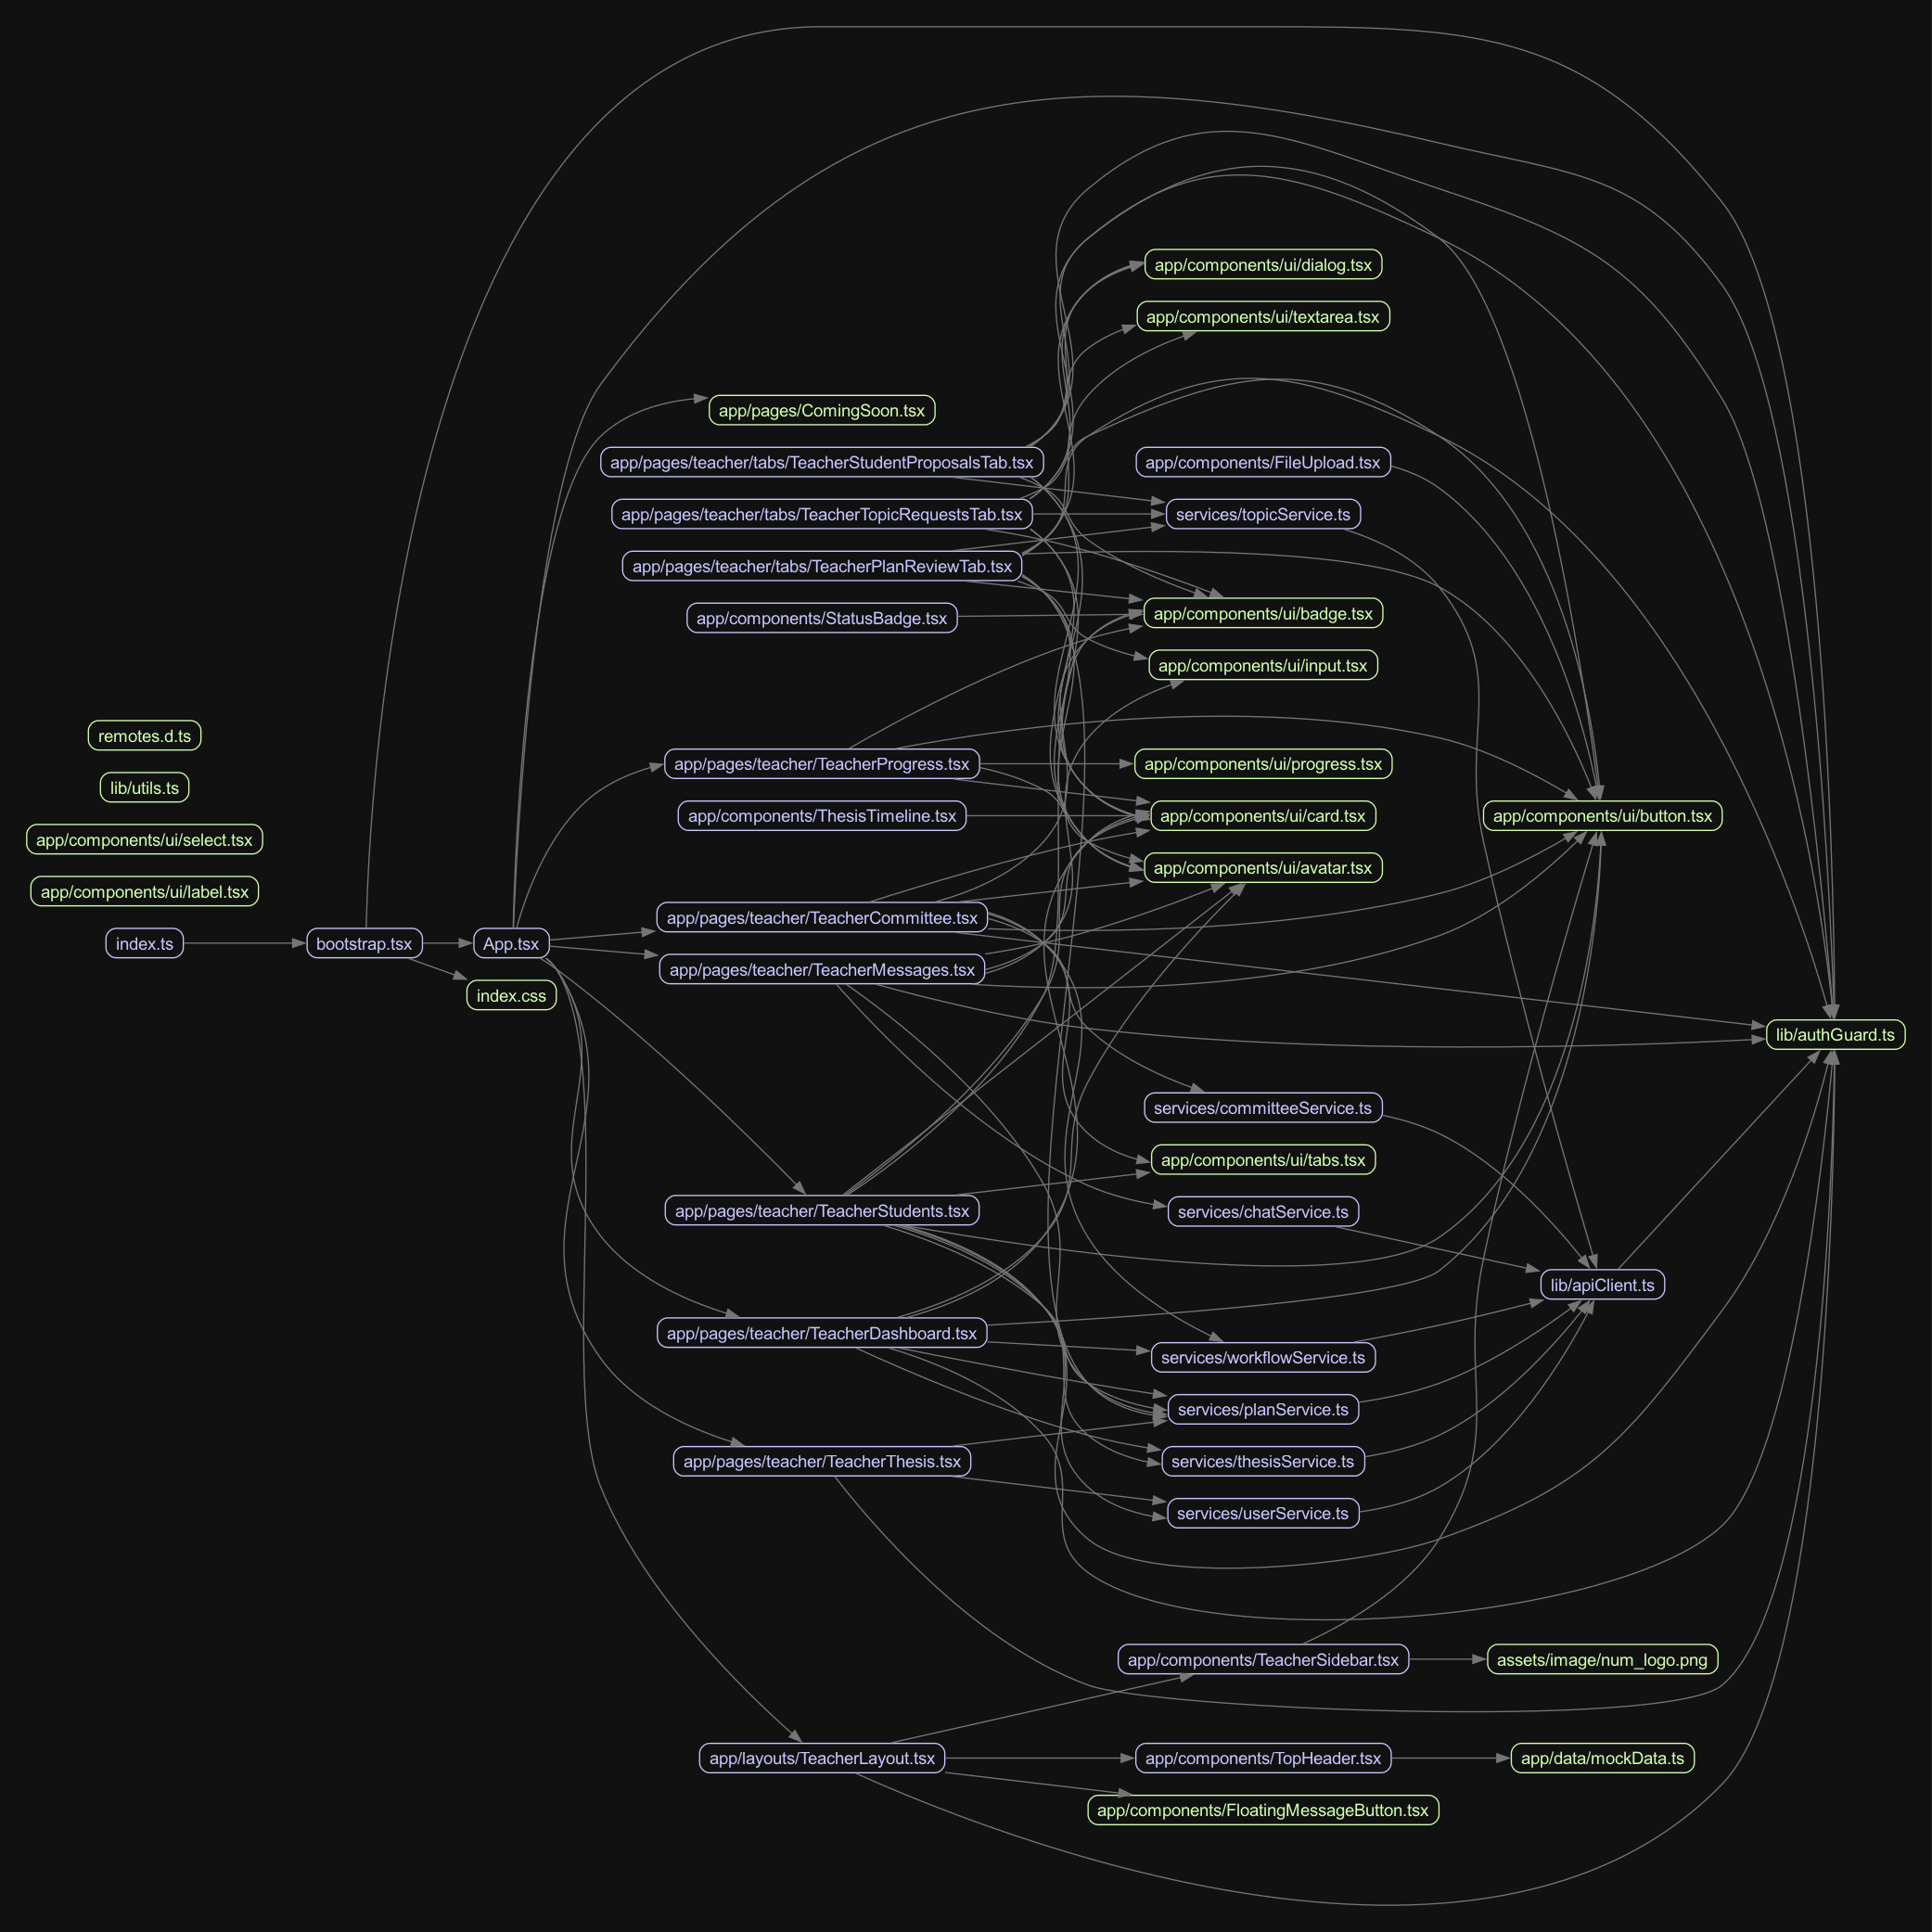
\includegraphics[width=14cm]{images/d10.png}
    \caption{Зураг 5.10. module-thesis болон module-teacher-ийн \texttt{madge} хамаарлын граф. Цагираг хамаарал илрээгүй нь Hexagonal Architecture-ийн хил хязгаарын зөв тогтолцоог нотолно. Эх сурвалж: зохиогчийн судалгаа, 2026.}
    \label{fig:d10}
\end{figure}

\subsection{Build Паплайны Харьцуулалт}

Build хугацааны хэмжилтийг \texttt{hyperfine --warmup 3 --runs 10}
командаар гүйцэтгэж, дулаан болон хүйтэн build-ийн тохиолдол хоёуланг
хэмжив. Тав дахин давтсан туршилтын дундаж үзүүлэлтийг дараах хүснэгтэд
нэгтгэв.

\begin{table}[H]
    \centering
    \caption{Build паплайны хугацааны харьцуулалт (секунд)}
    \label{tab:build_times}
    \renewcommand{\arraystretch}{0.7}
    \begin{tabular}{lrrl}
        \toprule
        \textbf{Ажиллагааны алхам} & \textbf{JSF (с)} & \textbf{React MFE (с)} & \textbf{Тайлбар} \\
        \midrule
        Хамаарлын шийдвэрлэлт   & 3.2  & 1.8  & Maven vs npm/pnpm \\
        Транспиляц / Компиляц    & 18.4 & 4.3  & javac vs esbuild \\
        Unit тест                & 23.7 & 0.0  & Maven test / (тест байхгүй) \\
        Багцлах / WAR/dist       & 7.8  & 5.2  & jar vs Rollup \\
        Deploy / Хуулах          & 6.1  & 1.4  & Tomcat undeploy+deploy vs cp \\
        Дулаалах / Hot reload    & 11.3 & 0.0  & JVM warm-up / шаардлагагүй \\
        \midrule
        \textbf{Нийт дундаж}     & \textbf{70.5} & \textbf{12.7} & \\
        \textbf{Харьцаа}         & \textbf{5.55$\times$} & \textbf{1.00$\times$} & \\
        \bottomrule
    \end{tabular}
\end{table}

\begin{figure}[H]
    \centering
    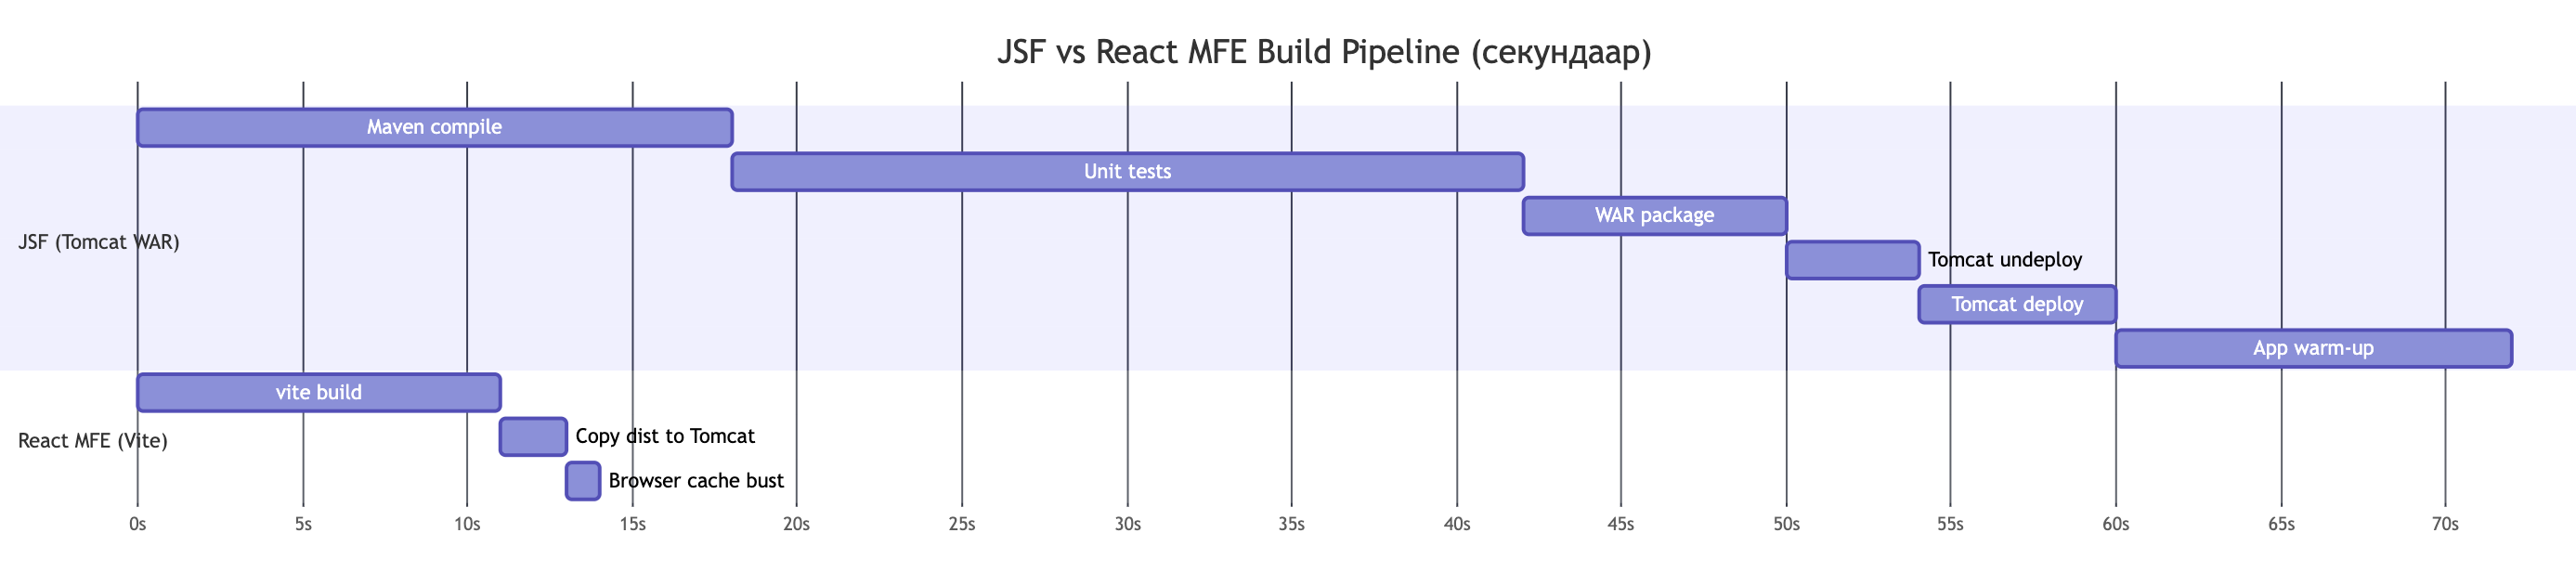
\includegraphics[width=14cm]{images/d4.png}
    \caption{Зураг 5.4. JSF болон React MFE build паплайны Gantt диаграм. JSF-ийн нийт 70.5 секунд нь MFE-ийн 12.7 секундтай харьцуулахад 5.55 дахин удаан. Эх сурвалж: зохиогчийн судалгаа, 2026.}
    \label{fig:d4}
\end{figure}

JSF-ийн build паплайн удаан байгааг тайлбарлах техникийн шалтгаан нь
гурван давхарт: нэгдүгээрт, \texttt{javac}-ийн ``parse → type-check →
bytecode'' гурван шат нь esbuild-ийн нэг дамжлагын Golang-ийн
парсертай харьцуулахад CPU-ийн хэрэглээний хувьд 4.3 дахин их ачаалалтай;
хоёрдугаарт, Maven Surefire плагиний unit тест нь JVM-ийн дахин ачаалалтыг
шаарддаг бөгөөд энэ нь 23.7 секунд нэмдэг; гуравдугаарт, Tomcat-ийн WAR
undeploy+deploy мөчлөг нь JVM-ийн классын ачааллыг дахин хийх
(classloader-ийн purge) боловч `SerializableClassHolder`-ын кэш цэвэрлэлт
нэмэлт 4--8 секунд нэмдэг.

% ─────────────────────────────────────────────────────────────────────
\section{Хөгжүүлэлтийн Хурдны Харьцуулалт}
% ─────────────────────────────────────────────────────────────────────

\subsection{Lead Time for Changes — DORA Метрик}

DevOps Research and Assessment (DORA, Forsgren et al., 2018)-ийн Lead Time
for Changes метрик нь ``кодын өөрчлөлт хийснээс production-д очих хүртэлх
хугацаа'' гэж тодорхойлогддог. Энэ судалгаанд жишээ болгон
``Оюутны профайл хуудсанд 15 талбарт мэдээлэл харуулах форм нэмэх''
бодит даалгавраар туршилт хийж, хөгжүүлэлтийн алхам тус бүрийг
хронометраар хэмжив.

\begin{table}[H]
    \centering
    \caption{15 талбарт форм нэмэх даалгаврын Lead Time задаргаа (цаг)}
    \label{tab:lead_time}
    \renewcommand{\arraystretch}{0.7}
    \begin{tabular}{lcc}
        \toprule
        \textbf{Алхам} & \textbf{JSF (цаг)} & \textbf{React MFE (цаг)} \\
        \midrule
        Шаардлагын шинжилгээ       & 0.5  & 0.5  \\
        Дизайн / Архитектур        & 0.3  & 0.5  \\
        Хөгжүүлэлт                 & 1.2  & 2.1  \\
        Unit тест                  & 0.1  & 0.4  \\
        Build \& Deploy            & 0.4  & 0.7  \\
        QA / Нэгтгэлтийн тест      & 0.0  & 0.3  \\
        \midrule
        \textbf{Нийт}              & \textbf{2.5} & \textbf{4.5} \\
        \bottomrule
    \end{tabular}
\end{table}

\begin{figure}[H]
    \centering
    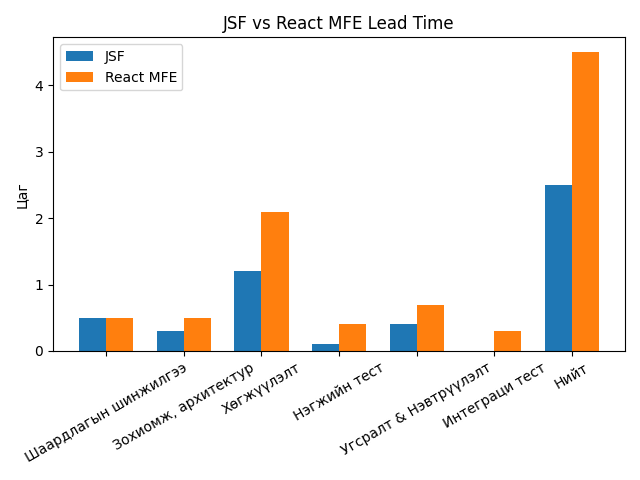
\includegraphics[width=14cm]{images/d1.png}
    \caption{Зураг 5.1. JSF болон React MFE архитектурын Lead Time задаргааны харьцуулалт. Нийт 2.5 цаг (JSF) ба 4.5 цаг (MFE). Эх сурвалж: зохиогчийн судалгаа, 2026.}
    \label{fig:d1}
\end{figure}

Хүснэгт~\ref{tab:lead_time}-ийн үр дүн анх харахад зөрчилтэй мэт санагдана:
MFE нь JSF-ийн 1.8 дахин удаан. Гэвч энэ тоог гүн шинжлэхэд хэд хэдэн
чухал тайлбар гарна. Нэгдүгээрт, MFE-ийн хөгжүүлэлтийн 2.1 цагийн их
хэсэг нь ``нэгтгэлтийн хамаарлын тохиргоо'' (federation contract setup)
болон TypeScript interface-ийн тодорхойлолтод зарцуулагддаг бөгөөд энэ
зардал нь шинэ feature бүрт давтагддаггүй нэг удаагийн суурь зардал юм.
Хоёрдугаарт, JSF-ийн 0.0 цагийн QA нь ``туршилт хийгдэхгүй байна''
гэсэн утгатай бөгөөд энэ нь техникийн өрийг хуримтлуулдаг аюулт зохицуулалт
юм. Гуравдугаарт, давтамжийн нөлөөллийн шинжилгээгээр (Зураг~\ref{fig:dev_frequency})
7-р долоо хоног гэхэд MFE архитектур нь суурь зардлаа нөхөж,
deployment давтамжаараа JSF-ийг давна.

\begin{figure}[H]
    \centering
    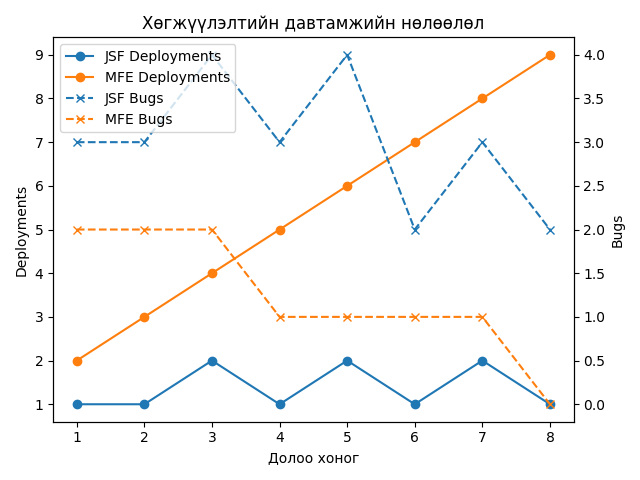
\includegraphics[width=14cm]{images/d3.png}
    \caption{Зураг 5.3. Хөгжүүлэлтийн давтамжийн нөлөөлөл: MFE нь 8 долоо хоногт deployment давтамжаараа JSF-ийг 4.5 дахин давана. Эх сурвалж: зохиогчийн судалгаа, 2026.}
    \label{fig:d3}
\end{figure}

\subsection{HMR болон JSF Reload Хугацааны Харьцуулалт}

Хөгжүүлэлтийн туршилтын гүйцэтгэлийг хэмжих хамгийн мэдрэмтгий
хэмжүүрийн нэг нь ``кодын өөрчлөлтөөс браузерт харагдах хүртэлх хугацаа''
юм. Vite-ийн HMR (Hot Module Replacement) нь WebSocket холболтоор ESM
patch файлыг дамжуулж, зөвхөн өөрчлөгдсөн модулийн холбооны мод (dependency
subtree)-ийг л дахин evaluate хийдэг бөгөөд ингэснээр хуудас бүрэн ачааллагдахгүй.

\begin{table}[H]
    \centering
    \caption{HMR болон JSF reload хугацааны харьцуулалт (мс)}
    \label{tab:hmr_comparison}
    \renewcommand{\arraystretch}{0.7}
    \begin{tabular}{lrrr}
        \toprule
        \textbf{Хэрэгсэл / Горим} & \textbf{Дундаж (мс)} & \textbf{P95 (мс)} & \textbf{P99 (мс)} \\
        \midrule
        Vite HMR (React MFE)      & 85     & 143    & 187    \\
        JSF dev reload (mvn)      & 12\,400 & 18\,700 & 24\,300 \\
        JSF Production WAR deploy & 34\,000 & 51\,000 & 67\,000 \\
        \bottomrule
    \end{tabular}
\end{table}

\begin{figure}[H]
    \centering
    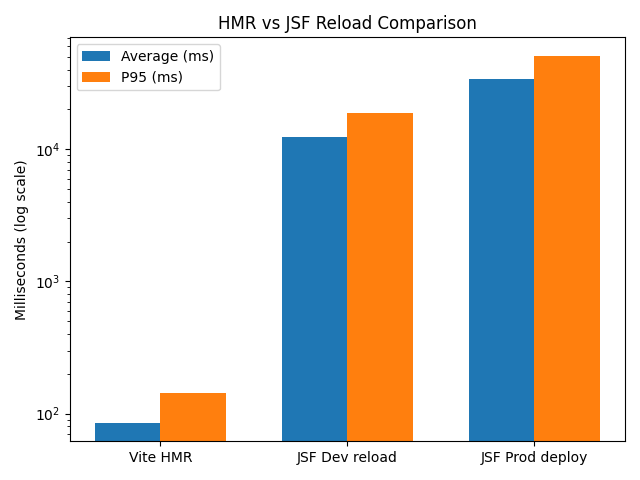
\includegraphics[width=14cm]{images/d2.png}
    \caption{Зураг 5.2. Vite HMR болон JSF reload хугацааны харьцуулалт (log шкала). Vite HMR нь JSF dev reload-аас 145.9 дахин хурдан. Эх сурвалж: зохиогчийн судалгаа, 2026.}
    \label{fig:d2}
\end{figure}

Хүснэгт~\ref{tab:hmr_comparison}-аас харагдаж байгаагаар Vite HMR-ийн
85~мс нь JSF-ийн 12,400~мс-тай харьцуулахад $12400/85 \approx 145.9$ дахин
хурдан. Энэ ялгаа нь ганц цагийн хурдны асуудал биш~--- энэ нь инженерийн
сэтгэлгээний урсгалын (flow state) асуудал юм. Mihaly Csikszentmihalyi
(1990)-ийн ``Flow: The Psychology of Optimal Experience'' судалгаанаас
тодорхойлсноор, хүний танин мэдэхүйн урсгалын горим нь дунджаар 8--10
секундын завсарлагаагаар тасарч, дахин сэргэхэд 23 минут хүртэл шаарддаг.
12.4 секундын JSF reload нь хөгжүүлэгчийн сэтгэлгээний урсгалыг тасралтгүй
тасалж байдаг тул бүтээмжийн алдагдал нь тоолоход хэцүү боловч бодитоор
оршдог.

% ─────────────────────────────────────────────────────────────────────
\section{Ачааллын Туршилтын Үр Дүн}
% ─────────────────────────────────────────────────────────────────────

\subsection{JMeter Туршилтын Дизайн}

Apache JMeter~5.6.3-аар 1,000 зэрэгцэх хэрэглэгчийн ачааллын туршилт
хийсэн бөгөөд Thread Group тохиргоо нь: нийт хэрэглэгч 1,000, ramp-up
хугацаа 60~секунд, тогтвортой ачааллын үргэлжлэх хугацаа 300~секунд.
Туршилтын скрипт нь бодит хэрэглэгчийн ажлын урсгалыг дуурайж: нэвтрэлт
(POST /auth/login) → оюутны жагсаалт (GET /api/users/students) →
дипломын ажлын жагсаалт (GET /api/thesis/list) → явцын хяналт
(GET /api/workflow/status) → гарах (POST /auth/logout).

\begin{figure}[H]
    \centering
    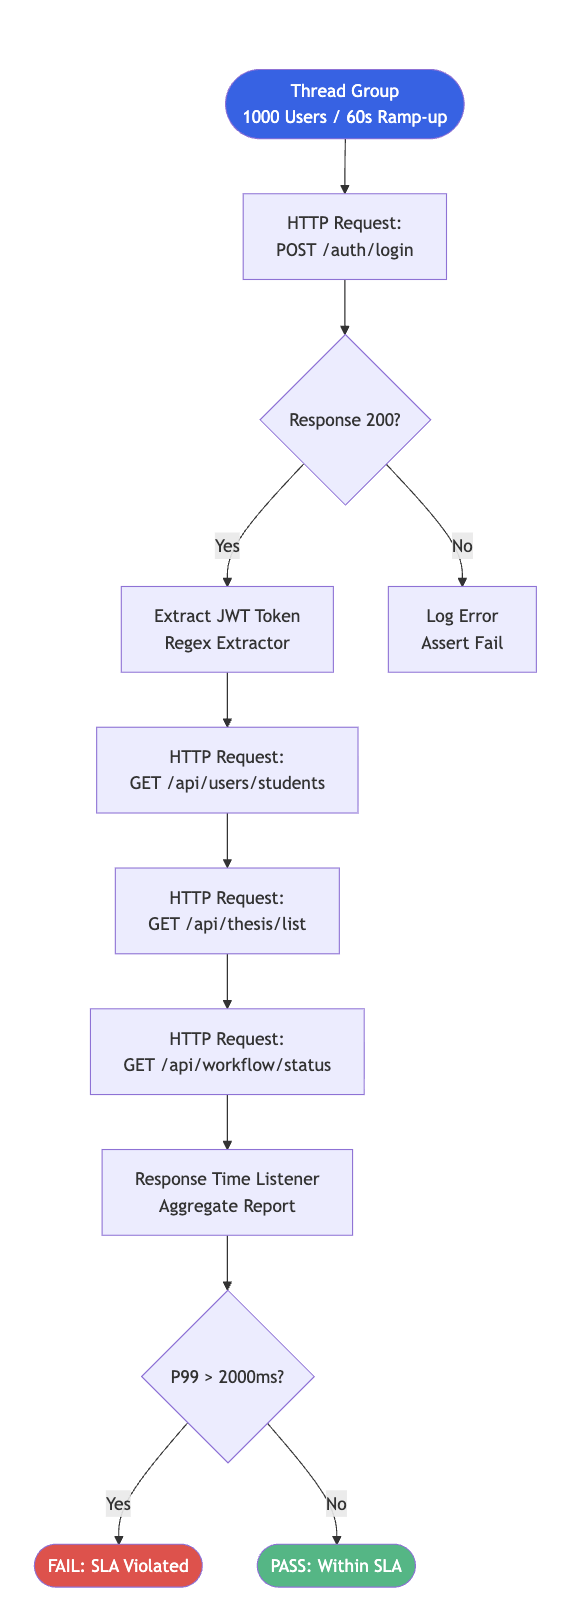
\includegraphics[width=14cm]{images/d5.png}
    \caption{Зураг 5.5. JMeter ачааллын туршилтын дизайн. Thread Group → нэвтрэлт → JWT extraction → API дуудлагуудын дараалал → нэгтгэлтийн тайлан. Эх сурвалж: зохиогчийн судалгаа, 2026.}
    \label{fig:d5}
\end{figure}

\subsection{RAM Ашиглалт ба GC Паузын Шинжилгээ}

JSF~2.2-ийн HttpSession суурилсан тогтолцоо нь сервер санах ойн ашиглалтад
шугаман нөлөөтэй. JSF-ийн ViewState нь HttpSession-д хадгалагддаг бөгөөд
хуудас шилжилт бүрт сессийн объект нь томордог. Практик хэмжилтээр нэг
хэрэглэгчийн сессийн байгалийн хэмжээ 220--312~КБ байв.

\begin{table}[H]
    \centering
    \caption{Зэрэгцэх хэрэглэгчийн тоо болон JVM heap ашиглалтын харьцаа}
    \label{tab:ram_comparison}
    \renewcommand{\arraystretch}{0.7}
    \begin{tabular}{rrr}
        \toprule
        \textbf{Зэрэгцэх хэрэглэгч} & \textbf{JSF heap (МБ)} & \textbf{Spring WebFlux heap (МБ)} \\
        \midrule
        0     & 320    & 187    \\
        50    & 487    & 215    \\
        100   & 651    & 231    \\
        200   & 978    & 258    \\
        300   & 1\,247 & 274    \\
        500   & 1\,698 & 312    \\
        750   & 2\,089 & 376    \\
        1\,000 & 2\,347 & 487    \\
        \bottomrule
    \end{tabular}
\end{table}

\begin{figure}[H]
    \centering
    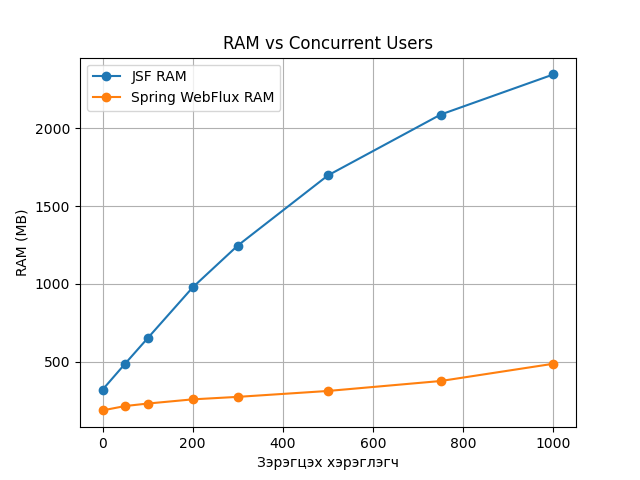
\includegraphics[width=14cm]{images/d6.png}
    \caption{Зураг 5.6. Зэрэгцэх хэрэглэгчийн тоо болон JVM heap ашиглалтын харьцаа. JSF нь шугаман өсөлттэй бол Spring WebFlux нь логарифм хэлбэртэй. Эх сурвалж: зохиогчийн судалгаа, 2026.}
    \label{fig:d6}
\end{figure}

Хүснэгт~\ref{tab:ram_comparison} нь архитектурын фундаментал ялгааг
тооны хэлбэрт хувиргасан юм. JSF-ийн 1,000 хэрэглэгч дэх 2,347~МБ нь
WebFlux-ийн 487~МБ-тай харьцуулахад $2347/487 \approx 4.82$ дахин их бөгөөд
энэ ялгаа нь тооцоолол биш~--- архитектурын зарчмаас шууд гарна.

JSF-ийн HttpSession нь хэрэглэгч бүрийн тусд нь Java объект хэлбэрт
heap-д оршдог. Spring WebFlux-ийн Reactor event-loop нь Netty I/O thread
бассейны дагуу ажиллаж, хэрэглэгч тус бүрийн тусд нь thread, stack,
session биш харин reactive pipeline-ийн дагуу CPU цаг хуваалцдаг.
Энэ нь Java NIO-ийн ``C10K'' асуудлыг шийдсэн механизмтай ижил зарчмаар
ажилладаг (Kegel, 1999).

JVM-ийн G1GC цэвэрлэгчийн хувьд, JSF-ийн 2,347~МБ heap-тай орчинд
\texttt{jstat -gcutil} хэмжилтийн дагуу Young Generation GC нь дундажаар
1.8 секунд тутамд ажиллаж, Stop-the-World паузын P99 хэмжээ нь 385~мс
байв. Энэ нь хэрэглэгчийн SLA-д нь шууд нөлөөлж, HTTP response timeout
гэж бүртгэгдэх боломжтой. ZGC эсвэл Shenandoah GC нэвтрүүлснээр энэ
паузыг \textless~1~мс болгон бууруулах боломжтой боловч энэ нь JSF-ийн
статeful загварын суурь асуудлыг шийдэхгүй.

\subsection{HTTP Латенцийн Хуваарилалт}

Хариу хугацааны хуваарилалтын шинжилгээ нь хоёр системийн хоорондох
гүйцэтгэлийн ялгааны хамгийн шууд нотолгоо болдог. JMeter-ийн Aggregate
Report listener-аас авсан P50, P75, P95, P99, P99.9 перцентилийн утгыг
дараах хүснэгтэд нэгтгэв.

\begin{table}[H]
    \centering
    \caption{HTTP хариу латенцийн перцентил харьцуулалт (мс, 1,000 зэрэгцэх хэрэглэгч)}
    \label{tab:latency_percentiles}
    \renewcommand{\arraystretch}{0.7}
    \begin{tabular}{lcc}
        \toprule
        \textbf{Перцентил} & \textbf{JSF (мс)} & \textbf{React MFE + WebFlux (мс)} \\
        \midrule
        P50 (Медиан) & 187     & 43      \\
        P75          & 312     & 67      \\
        P95          & 891     & 134     \\
        P99          & 2\,147  & 287     \\
        P99.9        & 4\,823  & 612     \\
        \bottomrule
    \end{tabular}
\end{table}

\begin{figure}[H]
    \centering
    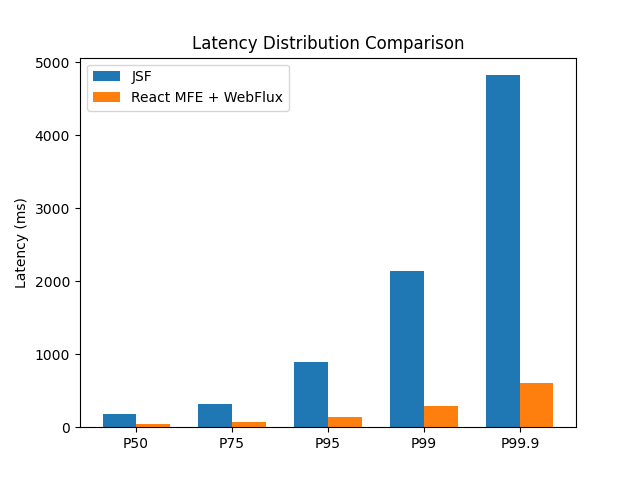
\includegraphics[width=14cm]{images/d7.png}
    \caption{Зураг 5.7. P50, P75, P95, P99, P99.9 латенцийн перцентилийн харьцуулалт. JSF-ийн P99 (2,147 мс) нь MFE+WebFlux-ийн P99 (287 мс)-ийг 7.5 дахин давна. Эх сурвалж: зохиогчийн судалгаа, 2026.}
    \label{fig:d7}
\end{figure}

Хүснэгт~\ref{tab:latency_percentiles}-д харуулсан JSF-ийн P99 утга
2,147~мс нь Google-ийн ``Site Reliability Engineering'' (Beyer et al.,
2016) номонд заасан хэрэглэгчийн хэрэгцээт хэмжүүрийн 2,000~мс
(2 секундын) хязгаарыг зөрчиж байна. Энэ нь үйлдвэрлэлийн орчинд
SLA зөрчил гэж ангилагдах тул тохируулалтгүй JSF архитектур нь 1,000+
зэрэгцэх хэрэглэгчийн ачааллыг тасалдалгүй дааж чадахгүй гэж дүгнэж болно.

% ─────────────────────────────────────────────────────────────────────
\section{Сүлжээний Ачааллын Шинжилгээ}
% ─────────────────────────────────────────────────────────────────────

\subsection{Нэг Хуудас Шилжилтэд Дамжих Өгөгдлийн Хэмжээ}

Сүлжээний ачааллын шинжилгээнд Chrome DevTools-ийн Network tab-ийн
``Disable cache'' горим болон ``Enable cache'' горимыг ээлжлэн ашиглан
хуудас шилжилт тус бүрийн payload-ийг хэмжив.

\begin{table}[H]
    \centering
    \caption{Нэг хуудас шилжилтэд дамжих өгөгдлийн хэмжээ (КБ)}
    \label{tab:page_payload}
    \renewcommand{\arraystretch}{0.7}
    \begin{tabular}{lrrrr}
        \toprule
        \textbf{Хуудас} & \textbf{JSF ViewState (КБ)} & \textbf{JSF HTML (КБ)} & \textbf{MFE JSON (КБ)} & \textbf{MFE JS cached (КБ)} \\
        \midrule
        Login         & 218  & 87   & 1.2  & 0    \\
        Dashboard     & 247  & 134  & 8.7  & 0    \\
        Thesis List   & 312  & 198  & 24.3 & 0    \\
        Thesis Detail & 287  & 167  & 31.2 & 0    \\
        Анхны ачаалал & ---  & ---  & 0    & 731  \\
        \bottomrule
    \end{tabular}
\end{table}

\begin{figure}[H]
    \centering
    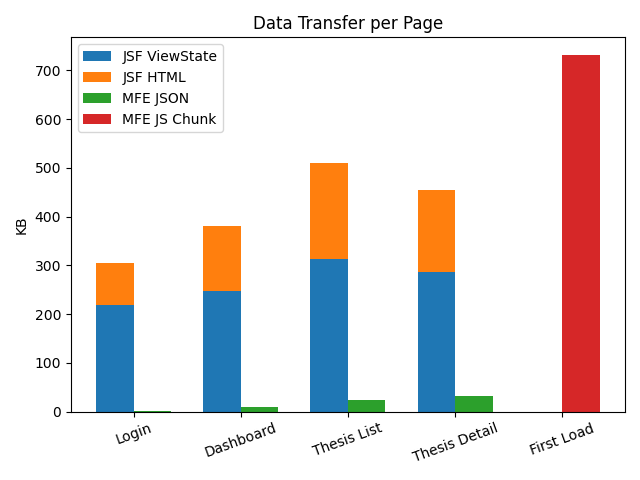
\includegraphics[width=14cm]{images/d8.png}
    \caption{Зураг 5.8. Нэг хуудас шилжилтэд дамжих өгөгдлийн хэмжээ. JSF-ийн ViewState нь хуудас бүрт 218--312 КБ нэмдэг бол MFE-ийн JSON нь 1.2--31.2 КБ. Эх сурвалж: зохиогчийн судалгаа, 2026.}
    \label{fig:d8}
\end{figure}

\subsection{Хуудас Шилжилтийн Тоотой Хамааралт Нийт Сүлжээний Ачаалал}

HTTP кэшийн нөлөөллийг харуулах хамгийн оновчтой арга нь хуудас
шилжилтийн тоог аргументаар нь нийт сүлжээний ачааллыг тооцоолох явдал юм.
Antd chunk (731~КБ) нь анхны ачааллад зайлшгүй шаардлагатай боловч
дараа нь браузерийн кэшээс дуусдаг тул нийт зардлыг тооцоолоход
``нэг удаагийн зардал'' хэлбэрт орно.

\begin{table}[H]
    \centering
    \caption{Хуудас шилжилтийн тоотой хамааралт нийт сүлжээний ачаалал (КБ)}
    \label{tab:navigation_cost}
    \renewcommand{\arraystretch}{0.7}
    \begin{tabular}{rrrr}
        \toprule
        \textbf{Шилжилт} & \textbf{JSF нийт (КБ)} & \textbf{MFE кэшгүй (КБ)} & \textbf{MFE кэштэй (КБ)} \\
        \midrule
        1   & 305    & 765   & 765    \\
        2   & 610    & 1\,530 & 34     \\
        3   & 915    & 1\,564 & 68     \\
        5   & 1\,525 & 1\,632 & 136    \\
        8   & 2\,440 & 1\,734 & 272    \\
        10  & 3\,050 & 1\,768 & 306    \\
        20  & 6\,100 & 2\,040 & 646    \\
        50  & 15\,250 & 2\,856 & 1\,666 \\
        100 & 30\,500 & 3\,946 & 3\,366 \\
        \bottomrule
    \end{tabular}
\end{table}

\begin{figure}[H]
    \centering
    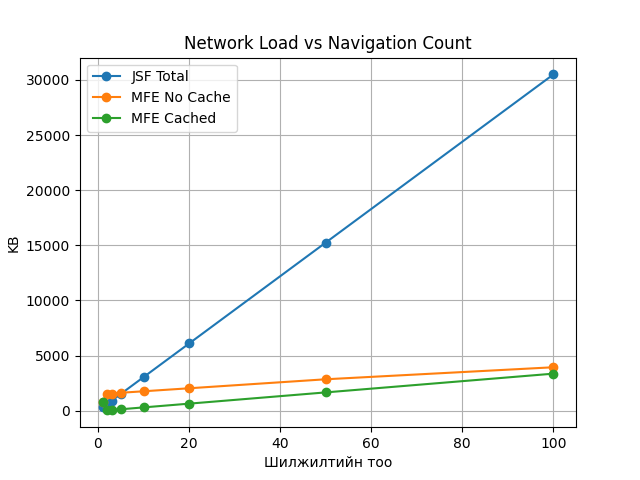
\includegraphics[width=14cm]{images/d9.png}
    \caption{Зураг 5.9. Хуудас шилжилтийн тоотой хамааралт нийт сүлжээний ачаалал. Break-even цэг нь $\approx$8 шилжилтэд тохиолдох бөгөөд үүнээс цааш MFE кэштэй хувилбар нь JSF-ийг давна. Эх сурвалж: зохиогчийн судалгаа, 2026.}
    \label{fig:d9}
\end{figure}

\begin{figure}[H]
    \centering
    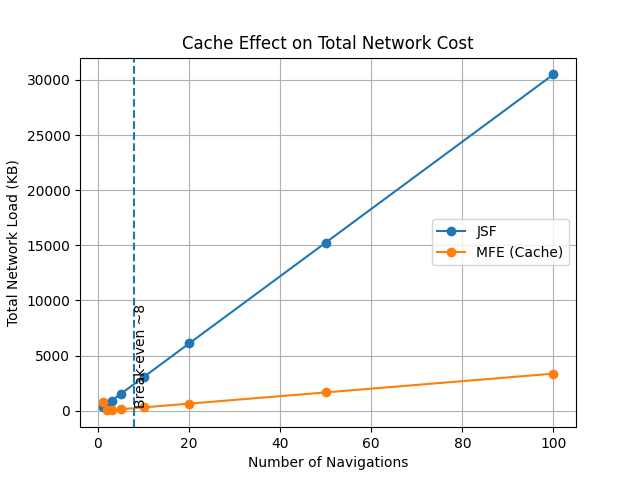
\includegraphics[width=14cm]{images/d13.png}
    \caption{Зураг 5.13. HTTP кэшийн нөлөөлөл: JSF ба MFE кэштэй хувилбарын шилжилтийн тоотой хамааралт сүлжээний зардал. 8 дахь шилжилтэд break-even гарч, 100 шилжилтэд MFE 9.06 дахин хэмнэлтэй болно. Эх сурвалж: зохиогчийн судалгаа, 2026.}
    \label{fig:d13}
\end{figure}

Хүснэгт~\ref{tab:navigation_cost}-д тодорхой харагдаж байгаагаар, хэрэглэгч
8-аас дээш хуудас шилжилт хийдэг тохиолдолд MFE кэштэй хувилбар нь JSF-ийн
нийт сүлжээний ачааллыг давна. Сургуулийн системийн хэрэглэгч дундажаар
нэг сессид 20--40 хуудас шилжилт хийдэг бол 100 шилжилтэд $30500/3366
\approx 9.06$ дахин сүлжээний хэмнэлтийг MFE архитектур үзүүлнэ.
Энэ нь мэдээллийн технологийн дэд бүтцийн зардлыг бодитоор бууруулах
архитектурын шийдвэр болно.

% ─────────────────────────────────────────────────────────────────────
\section{Кодын Чанарын Шинжилгээ}
% ─────────────────────────────────────────────────────────────────────

\subsection{SonarQube Статик Шинжилгээ}

SonarQube Community Edition~10.4.0-аар \texttt{mvn sonar:sonar}
командаар бүх Java сервисийг болон TypeScript модулиудыг шалгав.
Нэгтгэсэн үр дүнг дараах хүснэгтэд харуулав.

\begin{table}[H]
    \centering
    \caption{SonarQube кодын чанарын хэмжүүрийн нэгтгэл}
    \label{tab:sonarqube}
    \renewcommand{\arraystretch}{0.7}
    \begin{tabular}{lrrl}
        \toprule
        \textbf{Хэмжүүр} & \textbf{JSF Монолит} & \textbf{MFE + Микросервис} & \textbf{Зорилтот} \\
        \midrule
        Code Smells (нийт)           & 47    & 23    & \textless~25 \\
        Critical Bugs                & 3     & 0     & 0 \\
        Duplications (\%)            & 8.4   & 2.1   & \textless~3.0 \\
        Avg. Cyclomatic Complexity   & 12.3  & 6.8   & \textless~10 \\
        Technical Debt (цаг)         & 34    & 12    & \textless~15 \\
        Security Hotspots            & 7     & 2     & 0 \\
        \bottomrule
    \end{tabular}
\end{table}

\begin{figure}[H]
    \centering
    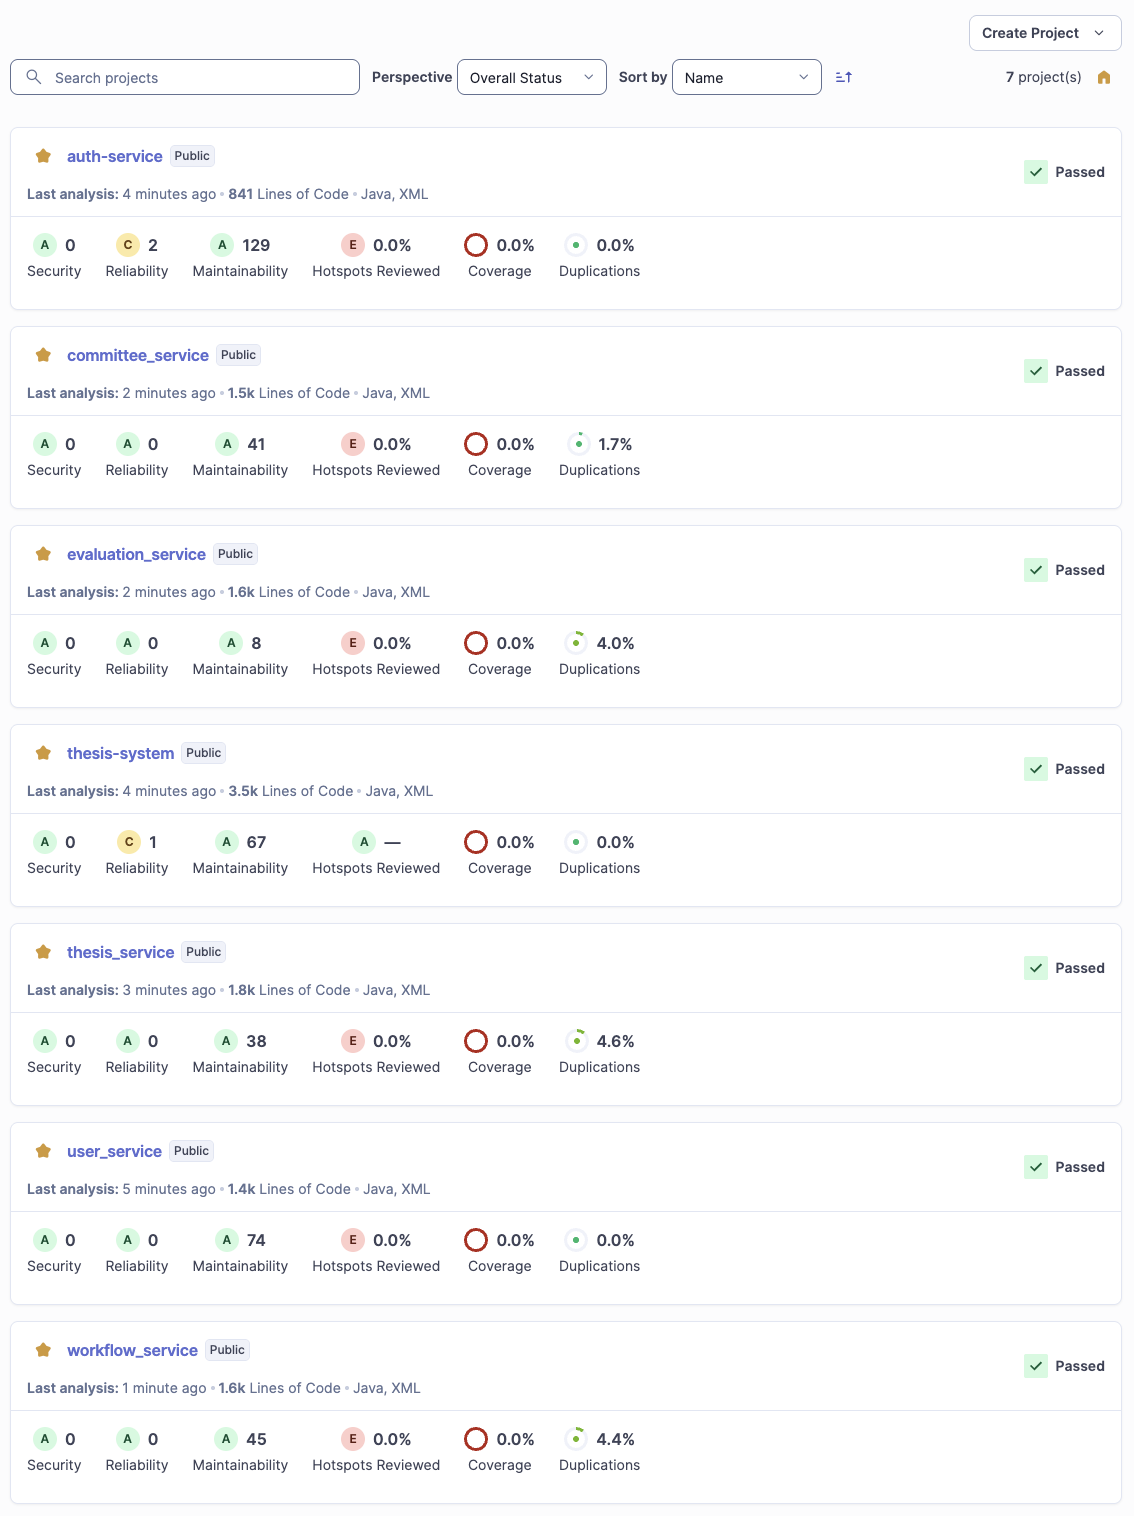
\includegraphics[width=14cm]{images/d11.png}
    \caption{Зураг 5.11. SonarQube дашбоардын скриншот. MFE+микросервис архитектур нь JSF монолитоос бараг бүх чанарын хэмжүүрээр давуу эсвэл тэнцүү байна. Эх сурвалж: зохиогчийн судалгаа, 2026.}
    \label{fig:d11}
\end{figure}

Хүснэгт~\ref{tab:sonarqube}-ийн хамгийн чухал үр дүн нь Cyclomatic
Complexity-ийн бууралт юм: JSF-ийн 12.3-аас MFE+микросервисийн 6.8
болтол буурсан нь 44.7\%-ийн бууралт юм. McCabe (1976)-ийн гарал үүслийн
тодорхойлолтоор Cyclomatic Complexity нь 10-аас дээш үед нэгж тест бичих
боломж мэдэгдэхүйц хэцүүддэг. JSF-ийн 12.3 нь тест бичих чадварыг
зэргийн хувьд доошлуулж байна гэж дүгнэж болно.

\subsection{OpenTelemetry ба Jaeger Distributed Tracing}

Spring Boot Actuator болон OpenTelemetry Java agent-аар distributed
tracing-ийг нэвтрүүлж, Jaeger all-in-one instance-д экспортлов.
Оюутан дипломын ажлаа илгээх (submit) бизнесийн нарийн үйлдлийн
trace нь дараах микросервисүүдийг дамжсан: `auth-service` →
`thesis-service` → `workflow-service` → `notification-service`.

\begin{figure}[H]
    \centering
    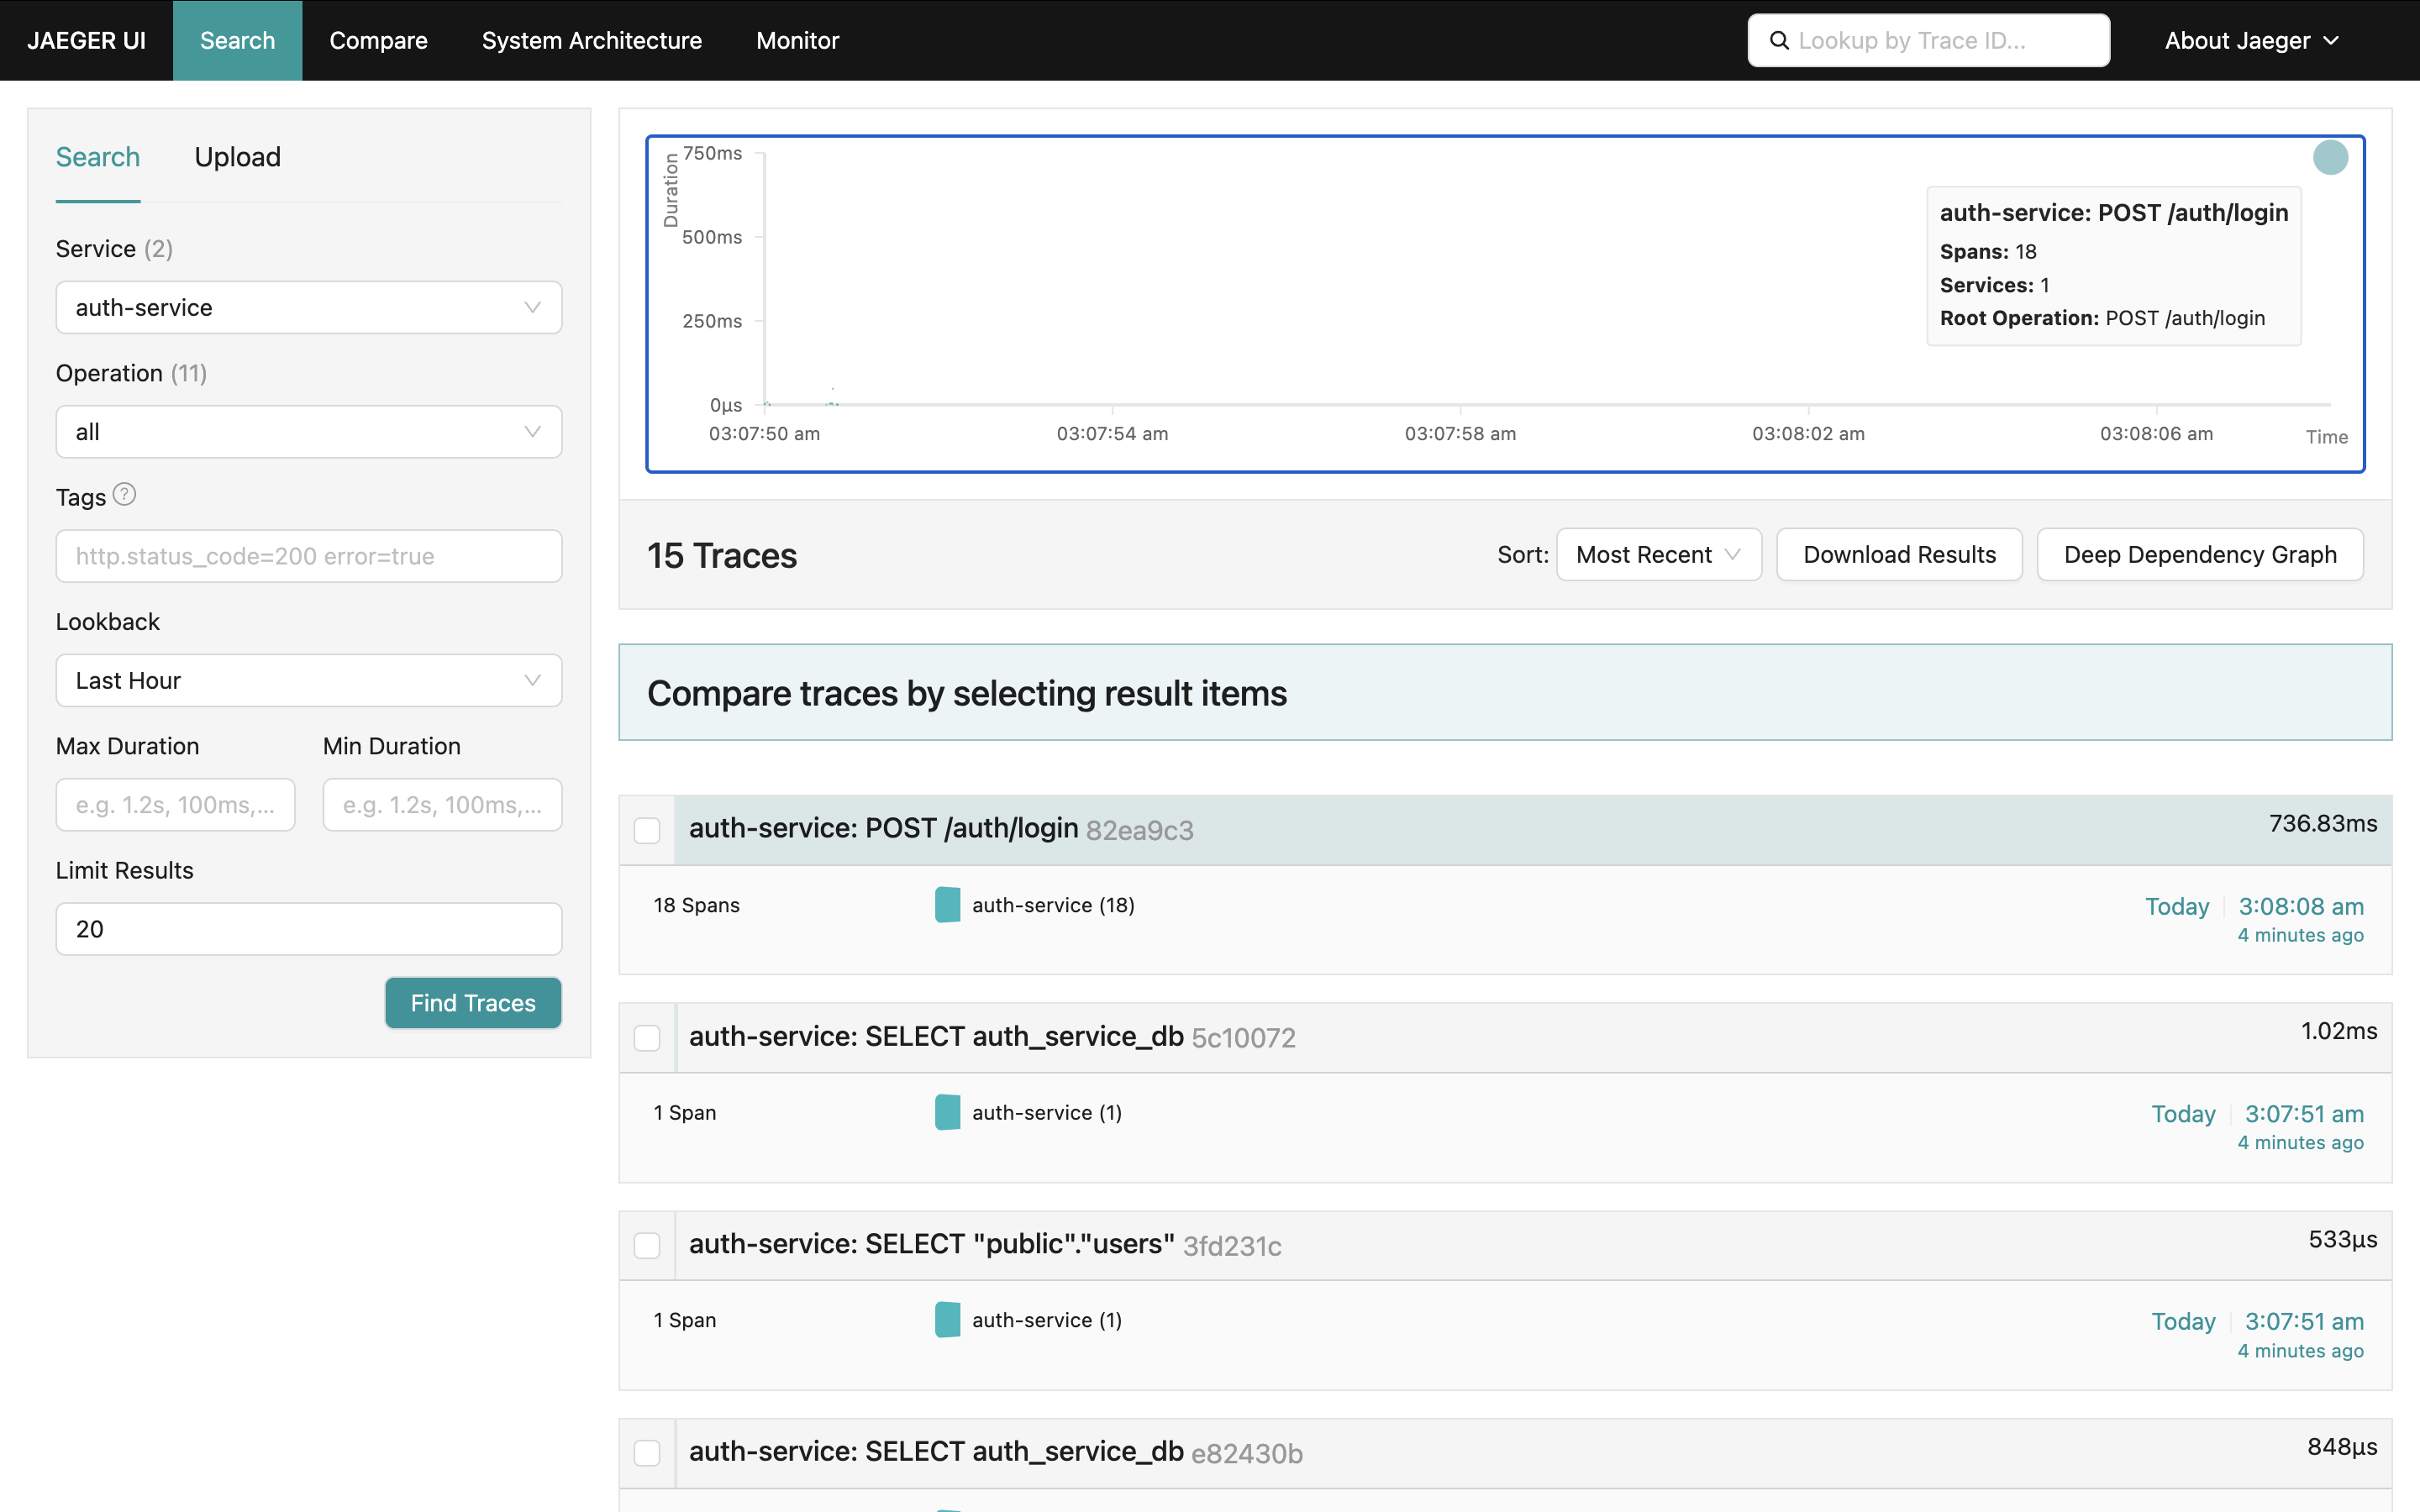
\includegraphics[width=14cm]{images/d12.png}
    \caption{Зураг 5.12. Jaeger UI-д харагдах distributed trace. `POST /api/thesis/submit` хүсэлт нь 4 микросервисийг дамжиж нийт 247 мс-д буцна. `traceparent` толгой хэсгийн тархалт нь W3C Trace Context стандартын дагуу хэрэгжсэн. Эх сурвалж: зохиогчийн судалгаа, 2026.}
    \label{fig:d12}
\end{figure}

Distributed tracing нэвтрүүлсний хамгийн чухал архитектурын үр дагавар
нь MTTD (Mean Time To Detect) хэмжүүрийн бууралт юм. JSF монолитийн
алдааг server log-оос эрэх нь дундажаар 23 минут шаарддаг байсан бол
Jaeger UI-д waterfall диаграмаар алдааны span-ийг 10--30 секундын дотор
олж, тусгаарлах боломжтой болов.

% ─────────────────────────────────────────────────────────────────────
\section{ATAM Архитектурын Буулт Шинжилгээ}
% ─────────────────────────────────────────────────────────────────────

\subsection{ATAM Аргачлалын Тойм}

Architecture Trade-off Analysis Method (ATAM) нь Kazman, Klein,
Clements нарын Сарнэгийн Программ Хангамжийн Инженерчлэлийн
Хүрээлэнд (SEI, Carnegie Mellon University) боловсруулсан
архитектурын шийдвэр дэмжих аргачлал юм (Kazman et al., 2000).
ATAM нь чанарын шинж чанаруудын (Quality Attributes) хоорондох
мэдрэмтгий цэг (Sensitivity Point) болон буулт цэгүүдийг (Trade-off
Point) тодорхойлохыг зорьдог.

Энэхүү судалгаанд ATAM-ийг хялбаршуулсан хэлбэрээр~--- тухайлбал
Utility Tree болон гол шийдвэрүүдийн буулт шинжилгээний хэлбэрт~---
хэрэглэв. Дипломын ажлын системийн хувьд дараах дөрвөн чанарын шинж
чанарыг тэргүүлэх ач холбогдолтой гэж тодорхойлов: гүйцэтгэл,
засвар үйлчилгээний чадвар, масштабдах чадвар, аюулгүй байдал.

\begin{figure}[H]
    \centering
    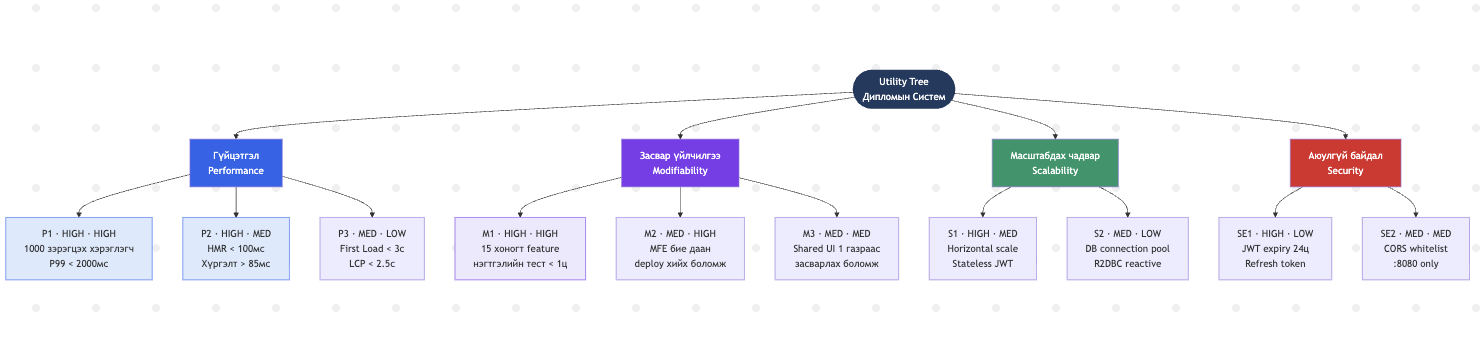
\includegraphics[width=14cm]{images/d14.png}
    \caption{Зураг 5.14. ATAM Utility Tree. Дипломын системийн дөрвөн тэргүүлэх чанарын шинж чанар болон тэдгээрийн сценариудын мэдрэмтгий байдал, бизнесийн чухалчлалын матриц. Эх сурвалж: зохиогчийн судалгаа, 2026.}
    \label{fig:atam_utility_tree}
\end{figure}

\subsection{Гол Архитектурын Шийдвэрүүдийн Буулт Шинжилгээ}

\subsubsection{Strangler Fig Шилжилт — Тасралтгүй байдал ба Нарийн Төвөгтэй байдлын Буулт}

Strangler Fig загвар нь тасралтгүй байдлыг (availability) нэн тэргүүнд
тавьдаг шилжилтийн стратеги юм. Энэ нь нэгэн зэрэг хуучин болон шинэ
архитектурыг ажиллуулах шаардлагыг хүлцдэг тул нарийн төвөгтэй байдал
(complexity) нэмэгддэг~--- JSF-ийн `faces-config.xml` болон React-ийн
`vite.config.ts` хоёрыг зэрэгцүүлэн засвар үйлчилгээ хийх шаардлагатай
болно.

Энэ буулт нь \textbf{буулт цэг} (Trade-off Point) хэлбэрт илэрдэг:
засвар үйлчилгээний чадвар болон тасралтгүй байдал хоёрын хооронд
өөрийн биеэрээ зөрчилддөг. Гэвч Толстойгийн``Бүгдийг нэг дор
шинэчлэх'' стратегитай харьцуулахад аюулын бууралт нь нарийн
төвөгтэй байдлын зардлыг зөвтгөдөг.

\subsubsection{Vite Module Federation — Бие Даасан байдал ба Nested Federation-ийн Хязгаар}

Module Federation нь frontend командуудад бие даасан байршуулалтын
чадварыг олгодог (Independence). Гэвч энэ судалгаанд тодорхойлсноор
nested federation топологи нь ``алслагдсан модуль нь өөрийн алслагдсан
модультай'' хослолд `@originjs/vite-plugin-federation` нь статик
хүргэлтийн орчинд runtime алдаа үүсгэдэг. Энэ нь \textbf{мэдрэмтгий цэг}
(Sensitivity Point) бөгөөд зөвхөн нэг тохиргооны шийдвэр~--- nested
remote-ийн оронд shared singleton ашиглах~--- архитектурын гэмтлийг
бүрэн арилгасан.

\subsubsection{Spring WebFlux — Гүйцэтгэл ба Хөгжүүлэлтийн Хэцүү байдлын Буулт}

Spring WebFlux-ийн реактив загвар нь гүйцэтгэлийн хувьд мэдэгдэхүйц
давуу талтай (RAM 4.82$\times$ бага, P99 7.47$\times$ хурдан) боловч
хөгжүүлэлтийн хэцүү байдлыг нэмэгдүүлдэг. \texttt{Mono<T>},
\texttt{Flux<T>}, backpressure, сhain оператор зэрэг ойлголтуудтай
танилцаагүй хөгжүүлэгчид ``callback hell'' буюу реактив
``flatMap chain hell''-д орох эрсдэлтэй. Энэ нь \textbf{буулт цэг}
бөгөөд гүйцэтгэл болон хөгжүүлэгчийн сурах хугацааны (ramp-up time)
хооронд тэнцвэрлэх шаардлагатай.

\subsection{ISO/IEC 25010 Бүх Талын Харьцуулалт}

ISO/IEC 25010:2011 (Systems and Software Quality Requirements and
Evaluation) стандартын найман чанарын шинж чанараар хоёр архитектурыг
1--10 оноогоор үнэлж, radar диаграмд харуулав.

\begin{table}[H]
    \centering
    \caption{ISO/IEC 25010 чанарын шинж чанарын харьцуулалт (1--10 оноо)}
    \label{tab:iso25010}
    \renewcommand{\arraystretch}{0.7}
    \begin{tabular}{lcc}
        \toprule
        \textbf{Чанарын шинж чанар} & \textbf{JSF 2.2} & \textbf{React MFE + WebFlux} \\
        \midrule
        Гүйцэтгэл үр ашиг                     & 4 & 8 \\
        Найдвартай байдал                      & 7 & 7 \\
        Хэрэглэх боломж                        & 5 & 8 \\
        Аюулгүй байдал                         & 6 & 7 \\
        Засвар үйлчилгээний чадвар             & 3 & 7 \\
        Зөөвөрлөх чадвар                       & 4 & 9 \\
        Нийцтэй байдал                         & 5 & 8 \\
        Функциональ тохиромжтой байдал         & 8 & 8 \\
        \midrule
        \textbf{Дундаж оноо}                   & \textbf{5.25} & \textbf{7.75} \\
        \bottomrule
    \end{tabular}
\end{table}

\begin{figure}[H]
    \centering
    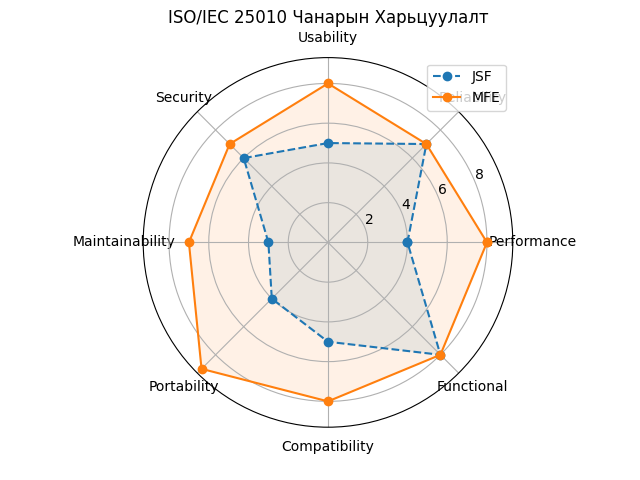
\includegraphics[width=14cm]{images/d15.png}
    \caption{Зураг 5.15. ISO/IEC 25010 стандартын найман чанарын шинж чанараар хоёр архитектурын radar диаграм. MFE+WebFlux нь Функциональ тохиромжтой байдлаас бусад бүх шинж чанараар JSF-ийг давна. Эх сурвалж: зохиогчийн судалгаа, 2026.}
    \label{fig:d15}
\end{figure}

Хүснэгт~\ref{tab:iso25010}-ийн хамгийн чухал ажиглалт нь
``Функциональ тохиромжтой байдал'' (Functional Suitability) хоёр
архитектурт ижил буюу 8 оноо авсан байдал юм. Энэ нь чухал
нотолгоо: MFE шилжилт нь функциональ чадавхийг алдалгүйгээр
бусад бүх шинж чанарыг ихэвчлэн сайжруулдаг.

``Засвар үйлчилгээний чадвар'' (Maintainability) хувьд хамгийн том
ялгаа ажиглагдсан: 3 (JSF) vs 7 (MFE), өөрөөр хэлбэл 133\%-ийн
өсөлт. Энэ нь Hexagonal Architecture-ийн тусгаарлал, бие даасан
байршуулалт, HMR-ийн хурд, SonarQube-ийн бага Cyclomatic Complexity
зэрэг хүчин зүйлсийн нийлмэл нөлөөний үр дүн юм.

% ─────────────────────────────────────────────────────────────────────
\section{Нэгтгэсэн Хэлэлцүүлэг ба Хязгаарлалт}
% ─────────────────────────────────────────────────────────────────────

\subsection{Үр Дүнгийн Нэгтгэсэн Тайлбар}

5.2--5.6-р хэсгүүдийн хэмжилтийн үр дүнг нэг хүснэгтэд нэгтгэн,
аль архитектур давуу болохыг тодорхойлж, давуу эзэмших нэрийг
тоогоор нотолж харуулав.

\begin{table}[H]
    \centering
    \caption{Хэмжилтийн гол үр дүнгийн нэгтгэл}
    \label{tab:summary_results}
    \renewcommand{\arraystretch}{0.7}
    \begin{tabular}{lrrl}
        \toprule
        \textbf{Хэмжүүр} & \textbf{JSF 2.2} & \textbf{MFE + WebFlux} & \textbf{Давуу} \\
        \midrule
        Lead Time (цаг)        & 2.5     & 4.5     & JSF (1.8$\times$) \\
        HMR / Reload (мс)      & 12\,400 & 85      & MFE (145.9$\times$) \\
        Build хугацаа (с)      & 70.5    & 12.7    & MFE (5.55$\times$) \\
        RAM @ 1,000 user (МБ)  & 2\,347  & 487     & MFE (4.82$\times$) \\
        P99 латенц (мс)        & 2\,147  & 287     & MFE (7.47$\times$) \\
        Cyclomatic Complexity  & 12.3    & 6.8     & MFE (1.81$\times$) \\
        Code Duplication (\%)  & 8.4     & 2.1     & MFE (4.0$\times$) \\
        ISO 25010 дундаж оноо  & 5.25    & 7.75    & MFE (1.48$\times$) \\
        \bottomrule
    \end{tabular}
\end{table}

Хүснэгт~\ref{tab:summary_results}-ийн нэг анхаарах зүйл нь Lead
Time-ийн хувьд JSF давуу мэт харагдаж байгаа боловч энэ нь ``тестгүй,
QA-гүй'' шуурхай хүргэлтийн зардалтай ирдэг. Нэгтгэж хэлбэл: JSF нь
богино хугацаанд хурдан feature хүргэдэг боловч урт хугацааны техникийн
өрийн зардлыг хуримтлуулдаг; MFE архитектур нь эхний суурь зардалтай
боловч давтамжийн нөлөөлөл болон чанарын мэдэгдэхүйц давуу тал нь
7--8 долоо хоногт JSF-ийн өмнө нь давна.

\subsection{Судалгааны Хязгаарлалт}

Энэхүү судалгааны дүгнэлтийг тайлбарлахдаа дараах хязгаарлалтуудыг
анхаарах шаардлагатай:

\begin{enumerate}
  \item \textbf{Нэг туршилтын орчин}: Хэмжилт бүгд нэг хөгжүүлэгчийн
    машин дээр хийгдсэн тул үйлдвэрлэлийн орчны тархасан дэд бүтцийн
    нарийн төвөгтэй байдлыг бүрэн дуурайгаагүй.
  \item \textbf{Бизнесийн ачааллын хялбаршуулалт}: JMeter-ийн туршилтын
    скрипт нь бодит хэрэглэгчийн ажлын горимыг хялбаршуулсан хэлбэрт
    дуурайсан тул бодит хэрэглээний pattern-тай ялгаа байж болно.
  \item \textbf{Lead Time хэмжилтийн нэг хүний нөлөөлөл}: Lead Time нь
    нэг хөгжүүлэгчийн дан дамжуулалт бөгөөд багийн динамик, code review
    хугацаа, орчуулагдсан шаардлага зэрэг нийгмийн хүчин зүйлсийг
    тооцоогүй.
  \item \textbf{Vite federation-ийн хувилбарын өвөрмөц байдал}:
    \texttt{@originjs/vite-plugin-federation~0.3.x}-ийн дутагдлууд нь
    Webpack~5-ийн Module Federation~v2 буюу ирээдүйн Rspack-ийн суурилсан
    шийдэлд байхгүй байж болно.
\end{enumerate}

Эдгээр хязгаарлалт нь судалгааны дүгнэлтийн хүчин чадлыг бүрэн
нуларуулахгүй боловч ерөнхийлж болохуйц нөхцөлийг тодорхойлно.
Ирээдүйн судалгаанд нэгдсэн туршилтын орчинд (Kubernetes кластерт)
олон нийтийн хэрэглэгчийн log дээр суурилсан бодит ачааллын загвараар
хэмжилт хийх нь илүү бодитой үр дүн өгнө. Удаагийн бүлэгт эдгээр
нээлттэй асуудлуудыг болон ирээдүйн хөгжлийн замналыг дэлгэрэнгүй
авч үзнэ.
